\documentclass[12pt,a4paper]{article}

\usepackage{polski}
\usepackage[polish]{babel}
%\usepackage[none]{hyphenat} %no hyphen breaks
\usepackage[utf8]{inputenc}

%font
\usepackage[sfdefault]{roboto} %% option 'sfdefault' activates Clear Sans as the default text font
\usepackage[T1]{fontenc}

\usepackage{color}

\usepackage{graphicx}

%justify - no hyphens
\tolerance=1000
\emergencystretch=\maxdimen
\hyphenpenalty=1000
\hbadness=10000

\usepackage{enumitem}
\setenumerate[1]{label=\Alph*.}
\setenumerate[2]{label=\roman*.}
\setenumerate[3]{label=\alph*.}
\setenumerate[4]{label=\arabic*.}

% Section numbering
\setcounter{secnumdepth}{5}
\setcounter{tocdepth}{2}

\usepackage{changepage}   % for the adjustwidth environment
\usepackage{letltxmacro}

% Unnumbered sections included in ToC
\newcommand{\psection}[1]{
  \section*{#1}
  \addcontentsline{toc}{section}{#1}
}
\newcommand{\psubsection}[1]{
  \subsection*{#1}
  \addcontentsline{toc}{subsection}{#1}
}

\usepackage[explicit]{titlesec}
\usepackage{ulem}
\titleformat{\section}{\normalfont\Large\bfseries}{\thesection.}{2ex}{#1}
\titleformat{\subsection}{\normalfont\large\bfseries}{\thesubsection.}{1.5ex}{#1}
\titleformat{\subsubsection}{\normalfont\normalsize\bfseries}{\thesubsubsection.}{1ex}{#1}
\titleformat{\paragraph}[block]{\normalfont\normalsize}{}{0pt}{\uline{\theparagraph\hspace*{1ex}#1}} %

%custom spacing
%\titlespacing*{\paragraph}{5em}{0pt}{0pt}

% Indent subsubsections
\newenvironment{indentpar}[1]%
  {\begin{list}{}%
          {\setlength{\leftmargin}{#1}}%
          \item[]%
  }
  {\end{list}}

% \LetLtxMacro{\oldsubsubsection}{\subsubsection}
% \renewcommand{\subsubsection}[1]{
%   \oldsubsubsection{#1}%
%   %\hangindent2em
%   %\hangafter=0
% }

% Custom subparagraphs
\definecolor{darkyellow}{RGB}{244,213,9}
\definecolor{darkgreen}{RGB}{96,221,42}
\newcommand\redcard[1]{\bgroup\textcolor{red}{\textbf{#1}}}
\newcommand\yellowcard[1]{\bgroup\textcolor{darkyellow}{\textbf{#1}}}
\newcommand\bluecard[1]{\bgroup\textcolor{blue}{\textbf{#1}}}
\newcommand\other[1]{\bgroup\textcolor{darkgreen}{\textbf{#1}}}

\usepackage{geometry}

\newcommand\image[2]{
	\newgeometry{left=0cm,top=#2}
	\includegraphics[width=\paperwidth]{#1}
	\restoregeometry
}

\setlength{\parindent}{0pt} % brak wcięć
\setlength{\parskip}{1ex plus 0.5ex minus 0.2ex}
\normalem %emphasis isn't underline
\linespread{1.1} %interlinia

\title{Zasady gry w~quidditcha}
\author{Polska Liga Quidditcha}
\date{Sezon 2017 - 2018}

\begin{document}

\maketitle

\setlength{\parskip}{0ex}

\tableofcontents

\setlength{\parskip}{1ex plus 0.5ex minus 0.2ex}

\newpage

\psection{Wstęp}

Popularność quidditcha stale rośnie i~rozwija się on w~dynamiczną i~ambitną dyscyplinę sportową, wymagającą nie lada wysiłku fizycznego,
złożonych strategii i~nielichych umiejętności.

Naturalnie, zasady gry muszą nadążać za nowymi wymaganiami, problemami i~sposobami gry. Muszą one przewidywać możliwe wyzwania i~być dostosowane
do wymogów bezpieczeństwa sportu, który rozwija się w~szybkim i~nieprzewidywalnym tempie.

Quidditch nie jest już sportem rozgrywanym jedynie w~przydomowych
ogródkach -- coraz częściej gra się na otwartej przestrzeni, przed
liczną widownią. Niezależnie od okoliczności i~warunków, zasady nie mogą
pozostawiać wątpliwości co do tego, jak ma wyglądać rozgrywka.

To wydanie \emph{Zasad gry w~quidditcha} opiera się o dziewiąte wydanie zasad USQ, większość zasad pozostała niezmieniona. Aczkolwiek wprowadzone zostały poprawki biorące pod uwagę grę na arenie międzynarodowej, kładąc nacisk na bezpieczeństwo i integralność rozgrywek.

Tym, którzy dopiero zaczynają swoją przygodę z~quidditchem, proponujemy,
by najpierw nauczyli się zasad gry od znajomych i~innych zawodników w~drużynie lub zapoznali się z~podstawowymi informacjami zawartymi w~rozdziale 1. Bardziej ambitnych oczywiście zapraszamy do lektury całości
\emph{Zasad gry w~quidditcha}.

Polska Liga Quidditcha dziękuje wszystkim zaangażowanym w~stworzenie
przekładu niniejszych \emph{Zasad} z~języka angielskiego. W
szczególności chcielibyśmy podziękować Klementynie Dec za nieocenioną
pomoc merytoryczną. Niemniej, tekst ten nie powstałby bez pracy i~poświecenia pozostałych członków grupy tłumaczeniowej. Serdecznie
dziękujemy (w kolejności alfabetycznej): Agacie Barszczewskiej, Maji Bartnik, Marianowi Dziubiakowi, Bognie Haponiuk, Paulinie
Rhone, Kindze Robutce, Jagodzie Sadeckiej i~Michałowi Szewczakowi.

\psubsection{Zasada czterech}

W czasie rozgrywki w~każdej drużynie quidditcha mogą być najwyżej cztery
osoby deklarujące tę samą płeć, pomijając szukającego. Płeć deklarowana
przez zawodnika może, ale nie musi, być tożsama z~jego płcią
biologiczną. Tę zasadę określa się mianem „zasady czterech''.

PLQ wraz z~IQA akceptują fakt, że nie wszyscy identyfikują się z~binarnym systemem podziału na płeć męską i~żeńską. PLQ i~IQA zapraszają
do gry wszystkich, niezależnie od ich tożsamości i~płci.

\image{team_poland}{6cm}

\pagebreak
\section{Podstawy gry}

\subsection{Quidditch}

Quidditch to koedukacyjny sport kontaktowy będący unikalną mieszanką
elementów rugby, zbijaka, zapasów, futbolu flagowego i~innych sportów.
Drużyna quidditcha składa się z~siedmiu zawodników, którzy przez cały
czas rozgrywki trzymają między nogami miotłę. Dla przypadkowego
obserwatora gra może się wydawać chaotyczna, jednak po zapoznaniu się z~podstawowymi zasadami quidditch staje się ekscytującym sportem do
oglądania, a~jeszcze bardziej ekscytującym, gdy osobiście włączy się do
gry.

\subsection{Pozycje}
Każda drużyna w~trakcie aktywnej gry składa się z~trzech ścigających,
dwóch pałkarzy i~jednego obrońcy. Pod koniec okna szukającego każda
drużyna wysyła do gry jednego szukającego.

\subsubsection{Ścigający}
Liczba ścigających w~grze na drużynę: trzech \\
Używana piłka: kafel \\
Kolor opaski: biały \\
Cel: rzucać, kopać lub w~inny sposób przerzucić kafel przez pętle
drużyny przeciwnej, by zdobyć 10 punktów

\subsubsection{Obrońcy}
Liczba obrońców w~grze na drużynę: jeden \\
Używana piłka: kafel \\
Kolor opaski: zielony \\
Cel: uniemożliwić przeciwnikowi rzucenie, kopnięcie lub w jakikolwiek inny sposób przerzucenie kafla przez pętle

\subsubsection{Pałkarze}
Liczba pałkarzy w~grze na drużynę: dwóch \\
Używana piłka: tłuczek \\
Kolor opaski: czarny \\
Cel: rzucać, kopać lub w~inny sposób za pomocą tłuczka zakłócać grę
przeciwników, poprzez ,,zbijanie'', czasowo eliminując ich z~gry

\subsubsection{Szukający}
Liczba szukających w~grze na drużynę: jeden \\
Używana piłka: znicz \\
Kolor opaski: żółty \\
Cel: odebrać znicz ludzkiemu zniczowi, by zdobyć 30 punktów i~zakończyć
część rozgrywki

\subsection{Rozgrywka}

\subsubsection{Zawodnicy grający kaflem}
\begin{enumerate}
	\item Ścigający i~obrońcy, zwani również zawodnikami grającymi kaflem,
	      usiłują zdobyć gola, i~powstrzymują przeciwną drużynę przed zdobyciem
	      punktów za pomocą kafla. Gol daje drużynie 10 punktów.

	\item Zawodnicy grający kaflem przemieszczają piłkę po boisku biegając z~nią, podając ją do współzawodników lub kopiąc.

	\item Zawodnicy grający kaflem bronią pętli poprzez odpowiednie ustawienie się lub inicjowanie
	      różnych form dozwolonego kontaktu fizycznego z~innymi zawodnikami.

	\item Obrońca w~swoim polu bramkowym jest odporny na zbicie i~posiada kilka
	      innych specjalnych uprawnień (patrz 7.3.3.2. Przywileje obrońcy).
	      W tym czasie obrońca uznawany jest za chronionego obrońcę. Pomijając tę różnicę, pozycja obrońcy nie różni się niczym od
	      ścigającego.
\end{enumerate}

\subsubsection{Pałkarze}
\begin{enumerate}
	\item Pałkarze używają piłek zwanych tłuczkami do zakłócania przebiegu gry
	      poprzez tymczasowe wyeliminowanie (,,zbicie'') tych zawodników drużyny
	      przeciwnej, którzy w~danym momencie gry nie są odporni na zbicie (patrz
	      5.2.8. Odporność na zbicie).

	\item Każdy zawodnik trafiony przez tłuczek posłany przez przeciwnika jest
	      wyłączony z~gry do czasu aż dokona procedury zbicia - chyba, że jest
	      odporny na zbicie (patrz 5.3 Procedura zbicia).
\end{enumerate}

\subsubsection{Szukający}
\begin{enumerate}
	\item Szukający usiłuje złapać piłkę zwaną zniczem poprzez odebranie jej
	      ludzkiemu zniczowi, aby zdobyć 30 punktów i~zakończyć część rozgrywki.

	\item Znicz jest piłką przymocowaną z~tyłu paska spodenek ludzkiego znicza
	      -- neutralnego zawodnika i~sędziego ubranego na żółto,
	      którego zadaniem jest nie dać się złapać przez jak najdłuższy czas,
	      jednocześnie pozostając sprawiedliwym dla obu drużyn.

	\item Złapanie znicza jest warte 30 punktów, a~jego zdobycie kończy część
	      rozgrywki. Mecz quidditcha składa się z~trzech części: „podstawowego
	      czasu gry'', „dogrywki'' i~„drugiej dogrywki''. Jeżeli w~danej części
	      rozgrywki po złapaniu znicza nastąpił remis, rozpoczyna się kolejna
	      część rozgrywki.
\end{enumerate}

\subsection{Faule}
Od wejścia na obszar gry, aby wziąć udział w rozgrywce, aż do chwili jej zakończenia, zawodnicy nie mogą wykonywać niedozwolonych akcji zwanych faulami. Ci, którzy je popełnią, zostają ukarani adekwatnie do wagi wykroczenia: 

\subsubsection{Powrót do pętli}
Powrót do pętli oznacza, że
zawodnik musi zaprzestać każdej innej aktywności i~powrócić do pętli - tak jak
w przypadku zbicia (patrz 5.3. Procedura zbicia).

\subsubsection{Niebieska kartka}
Niebieska kartka oznacza, że
zawodnik musi spędzić jedną (1) minutę na ławce kar, a jego drużyna gra w tym czasie w osłabionym składzie. Jeżeli drużyna przeciwna zdobędzie punkty przed upływem tej minuty, zawodnik zostaje uwolniony z ławki kar wcześniej i może kontynuować grę. Niebieskie kartki nie „kumulują się” do wyższych kar. 

\subsubsection{Żółta kartka}
Żółta kartka oznacza, że zawodnik musi spędzić jedną minutę (1) na ławce kar, a jego drużyna gra w tym czasie w osłabionym składzie. Jeżeli drużyna przeciwna zdobędzie punkty przed upływem tej minuty, zawodnik zostaje uwolniony z ławki kar wcześniej i może kontynuować grę. Żółte kartki „kumulują się” do wyższych kar – zawodnik który zostanie dwukrotnie ukarany żółtą kartką w jednym meczu, zostaje ukarany czerwoną.

\subsubsection{Czerwona kartka}
Czerwona kartka oznacza, że zawodnik zostaje wycofany z gry w danym meczu, a jego drużyna musi grać w osłabionym składzie przez dwie (2) pełne minuty czasu gry.

\subsubsection{Usunięcie}
Sędzia może usunąć zawodnika z~gry za
szczególnie poważne wykroczenie przeciwko zasadom gry.

\subsection{Zasada czterech}
W czasie rozgrywki w każdej drużynie quidditcha mogą być co najwyżej cztery osoby identyfikujące się z tą samą płcią, włączając w to szukającego po jego wejściu na boisko. Płeć, z którą identyfikuje się zawodnik jest uznawana za płeć tego zawodnika i może, ale nie musi, być tożsama z jego płcią biologiczną. Tę zasadę określa się mianem „zasady czterech”.

IQA wraz z PLQ akceptuje wszystkich, którzy nie identyfikują się z binarnym podziałem płci i rozumie, że nie wszyscy zawodnicy identyfikują się jako mężczyzna lub kobieta. IQA wraz z PLQ zapraszają do gry wszystkich, niezależnie od ich tożsamości i płci.

%\pagebreak
\thispagestyle{empty}
\newgeometry{left=2cm,top=2cm}
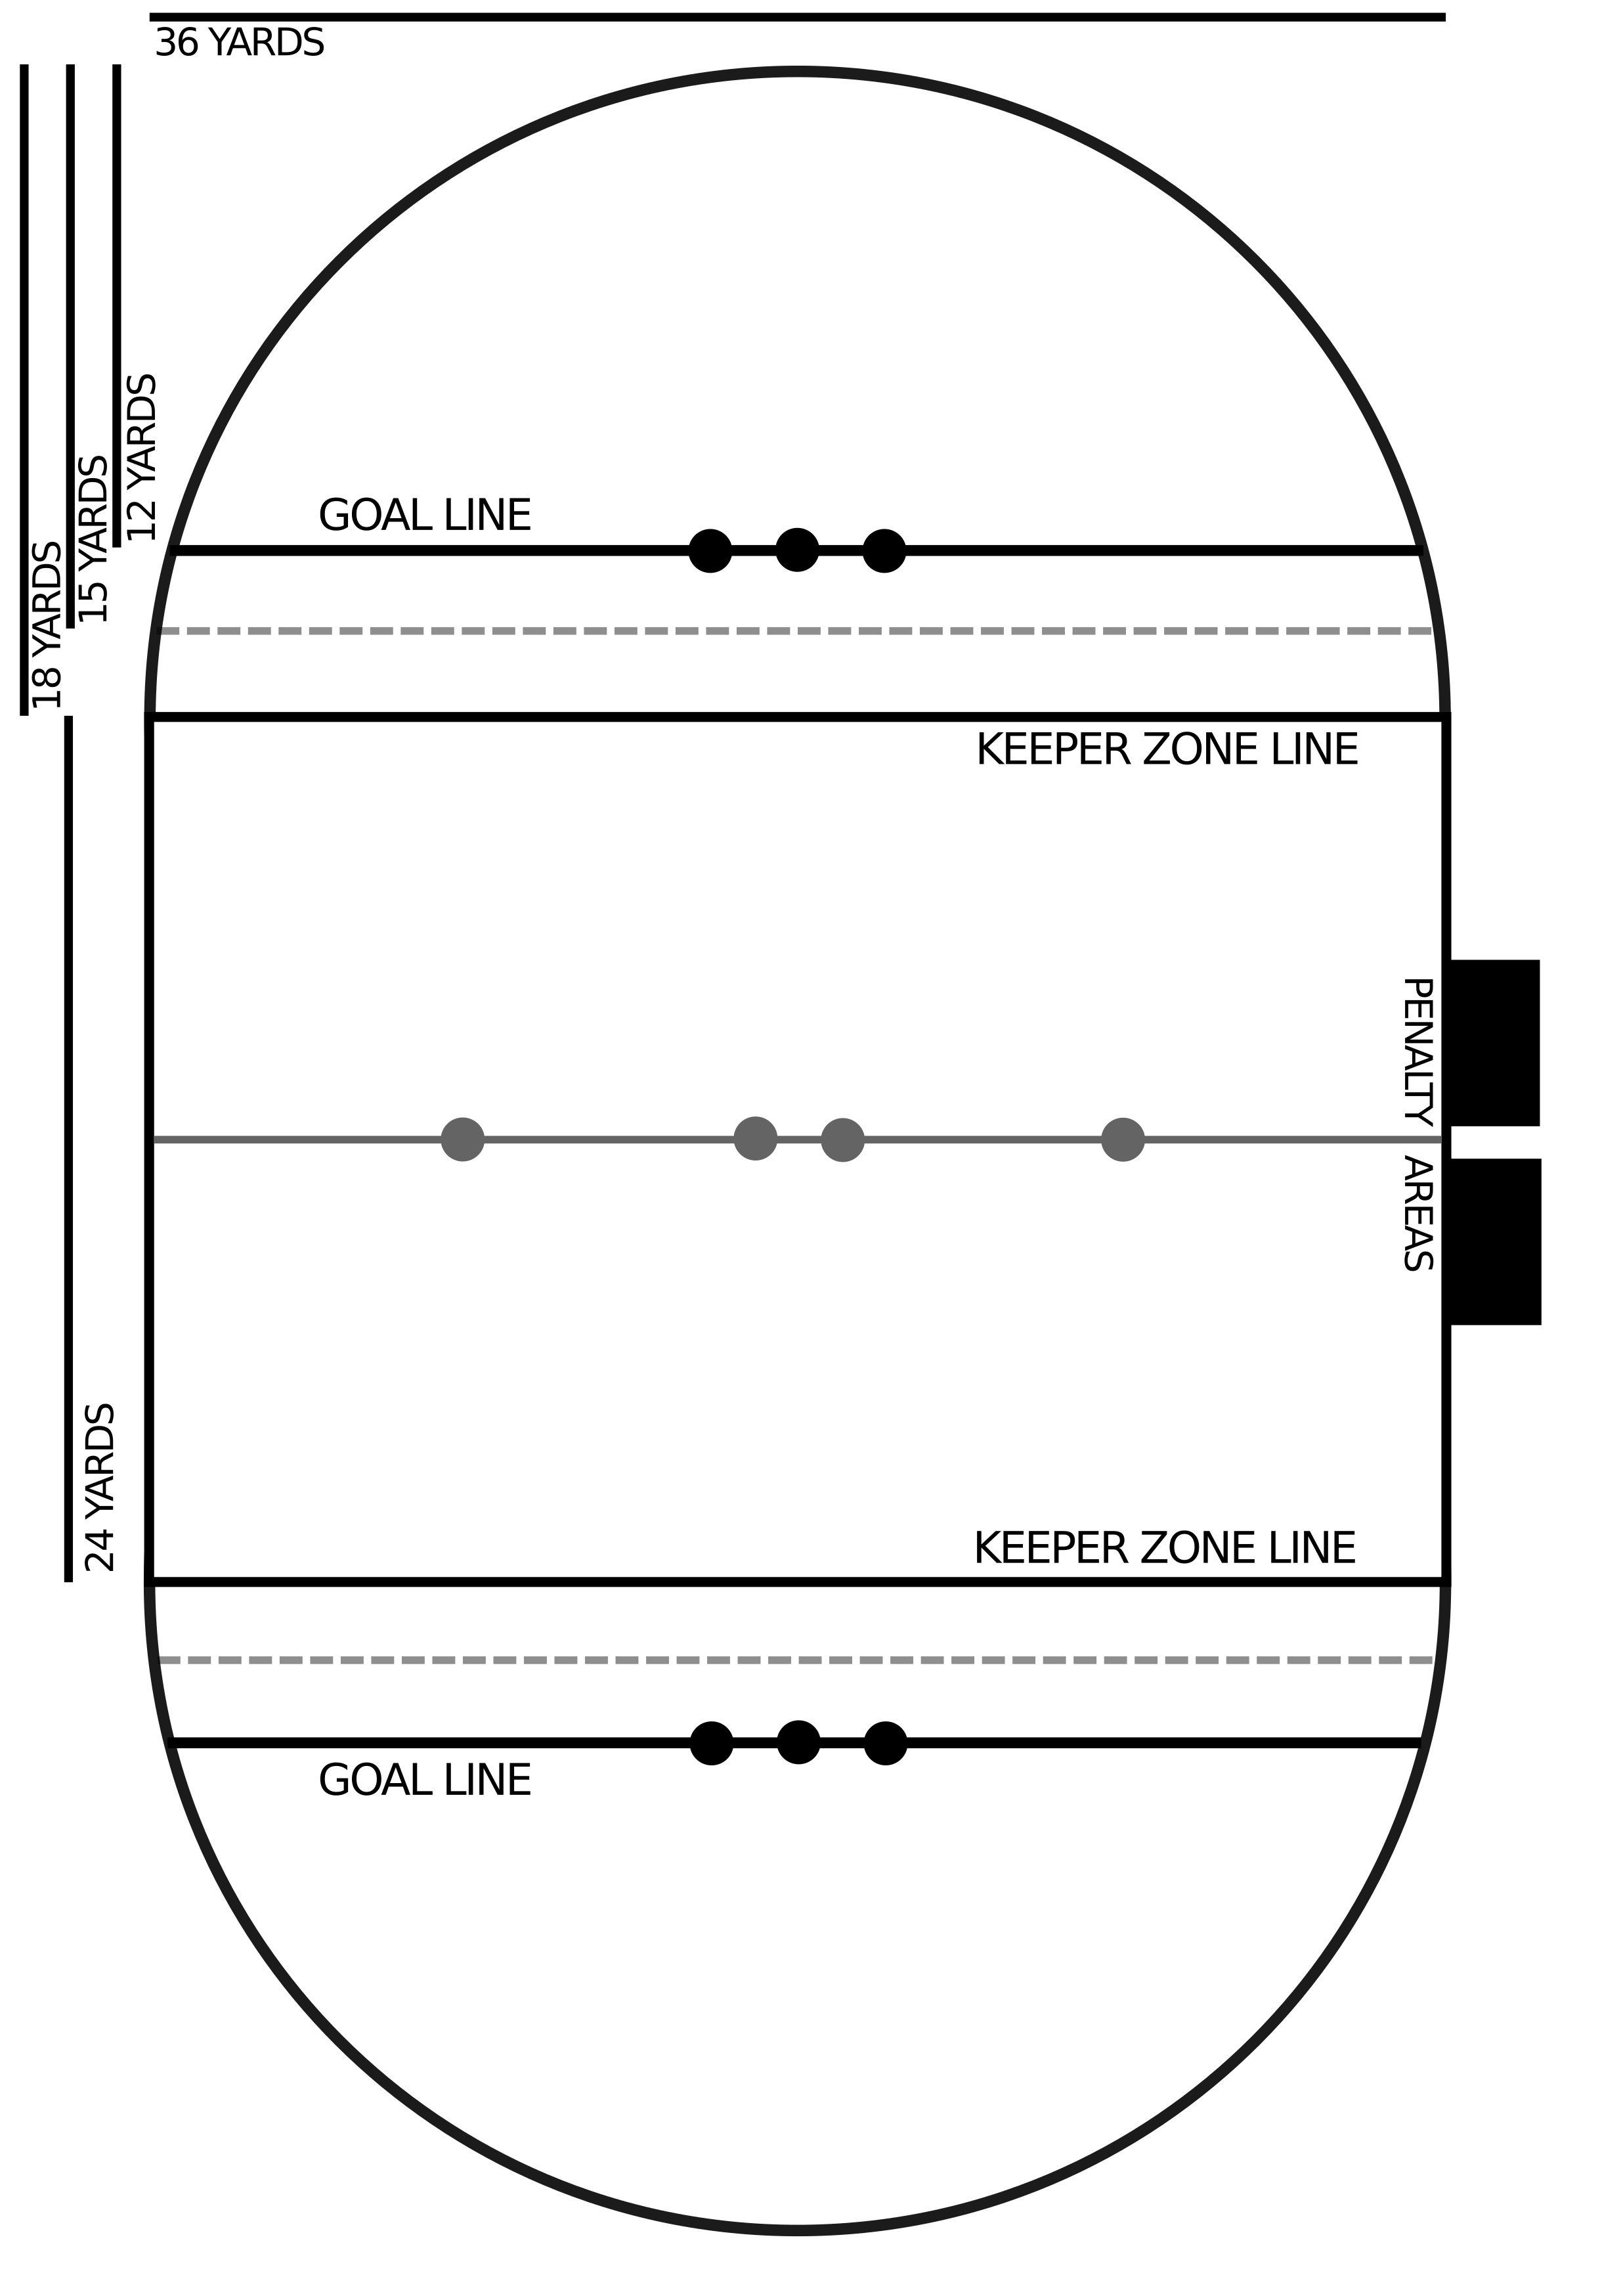
\includegraphics[width=0.8\paperwidth]{quidditch_pitch}
\restoregeometry

\pagebreak
\section{Wyposażenie i~wymiary boiska}

\subsection{Boisko}

\subsubsection{Kształt boiska}
Boisko składa się z~trzech części: prostokąta i~dwóch półokręgów na jego
krótszych bokach, co w~sumie tworzy kształt wydłużonego owalu. Chociaż
granice te wyznaczają pożądany kształt boiska, zawodnicy nie są
ograniczeni do przebywania wyłącznie na tym obszarze.
\begin{enumerate}
	\item{Linie boczne i~linie pola bramkowego} -- Prostokąt wyznacza
	      główną część boiska. Jego boczne krawędzie stanowią linie boczne, a~górna i~dolna krawędź -- linie pola bramkowego boiska.

	\item{Linie i~punkty końcowe} -- Linie końcowe boiska to
	      półokręgi biegnące od jednego do drugiego końca linii pola bramkowego.
	      Środek tej linii wyznacza najdalszy punkt pola bramkowego czyli punkt końcowy. Na boisku są dwie linie końcowe oraz dwa punkty końcowe.

	\item{Linia środkowa i~środek boiska} -- Boisko podzielone
	      jest w~poprzek na pół linią środkową przechodzącą przez dwa punkty środkowe linii bocznych. Środek boiska zaznaczony jest w~połowie linii środkowej.
\end{enumerate}

\subsubsection{Wymiary boiska}
Wymiary boiska (patrz 2.1.1) są następujące:
\begin{enumerate}
	\item{Linie boczne:}
	      \begin{enumerate}
		      \item Długość linii bocznej, czyli bocznej krawędzi prostokąta stanowiącego
		            główną część boiska (od jednego do drugiego pola bramkowego) to 22 m.

		      \item Szerokość prostokąta (czyli długość linii środkowej i~obydwu linii
		            pola bramkowego) to 33 m.
	      \end{enumerate}
	\item{Linie końcowe:}
	      \begin{enumerate}
		      \item Średnica półokręgu (długość linii pola bramkowego) to 33 m.

		      \item Promień półokręgu (od linii pola bramkowego do punktu końcowego) to
		            16,5 m.
	      \end{enumerate}
	\item{Inne wymiary:}
	      \begin{enumerate}
		      \item Długość boiska pomiędzy punktami końcowymi: 55 m.

		      \item Odległość pomiędzy zestawami bramek: 33 m.
	      \end{enumerate}
\end{enumerate}

\subsubsection{Pole bramkowe}
\paragraph{Linie pola bramkowego}
Dwie linie, które koniecznie
muszą być zaznaczone, łączące linie boczne boiska, równoległe do linii
środkowej. Znajdują się one w~odległości 16,5 m od punktu końcowego
boiska oraz 11 m od linii środkowej.

\paragraph{Zasięg pola bramkowego}
Chociaż linie pola bramkowego zaznaczone są tylko w obrębie głównej części boiska, rozciągają się one aż do granicy widowni po obu jego stronach. Obydwa pola bramkowe ciągną się od linii pola bramkowego w kierunku punktu końcowego boiska i dalej, aż do granicy widowni.

\paragraph{Pole bramkowe własne i~drużyny przeciwnej}
Własne pole bramkowe drużyny zawiera jej pętle. Pole bramkowe drużyny
przeciwnej zawiera pętle, przez które drużyna musi przerzucić piłkę,
żeby zdobyć punkt.

\subsubsection{Ławki kar}

\paragraph{Ławki kar}
Każda drużyna musi mieć wyznaczone miejsce
na ławkę kar. Obszar ten musi:
\begin{enumerate}
	\item Znajdować się po tej samej stronie boiska, co skryba.

	\item Znajdować się po tej samej stronie linii środkowej boiska, co ławka
	      drużyny.

	\item Znajdować się w obszarze gry, ale poza granicą boiska. Ławka kar każdej z drużyn jest kwadratem o wymiarach 5,5 m na 5,5 m, rozpoczynającym się przy linii środkowej boiska i rozciągającym się wzdłuż linii bocznej boiska w kierunku ławki drużyny.
\end{enumerate}

\paragraph{Rozmiar obszarów ławki kar i~ich rozmieszczenie można
	modyfikować w~zależności od wymagań skryby.}

\subsubsection{Strefa rezerwowych}

\paragraph{Strefy rezerwowych}
Każda drużyna musi mieć
wyznaczoną strefę rezerwowych. Każda taka strefa to obszar o~nieregularnym kształcie, które wyznaczone jest przez: granicę boiska,
granicę pola bramkowego oraz granicę obszaru gry. Strefa rezerwowych
musi być częścią obszaru gry i~pozostawać poza granicami boiska.

\begin{enumerate}
	\item Granice stref rezerwowych:
	      \begin{enumerate}
		      \item Linia końcowa boiska w~ramach pola bramkowego.

		      \item Granica obszaru gry w~ramach pola bramkowego, za wyjątkiem:
		            \begin{enumerate}
			            \item Zmiana zawodników powinna mieć miejsce poza obszarem wyznaczonym jako
			                  ławkę drużyny.
		            \end{enumerate}
	      \end{enumerate}

	\item Zawodnicy będący wewnątrz strefy rezerwowych:
	      \begin{enumerate}
		      \item Zawodnicy i~personel drużyny mogą opuszczać i~powracać do strefy
		            rezerwowych podczas rozgrywki, ale nie mogą pozostawać na dłużej poza
		            ławką drużyny.
	      \end{enumerate}
\end{enumerate}

\paragraph{Ławki drużyn}
Ławka drużyny to obszar wewnątrz strefy
rezerwowych, wewnątrz którego powinni przez większość czasu gry
pozostawać wszyscy zawodnicy i~personel drużyny, poza kapitanem
kontaktowym, którzy nie są aktywni w~grze lub nie mają zamiaru wkrótce
dołączyć do gry.

\begin{enumerate}
	\item Niżej wymienione osoby oraz wyposażenie muszą pozostawać wewnątrz
	      obszaru ławki drużyny:

	      \begin{enumerate}
		      \item Wszyscy zawodnicy rezerwowi, którzy nie mają zamiaru wkrótce
		            dołączyć do gry lub opuścili grę.
		      \item Personel drużyny oraz trenerzy, wyłączając kapitana odpowiedzialnego
		            za komunikację.
		      \item Wszelkie dodatkowe wyposażenie należące do drużyny, wyłączając
		            dodatkowe miotły, które nie mogą się znajdować w~obszarze gry i~muszą być przechowywane przy stole skryby.
	      \end{enumerate}

	\item Ławka drużyny powinna być prostokątem o~wymiarach 12 m na 2 m,
	      znajdującym się wewnątrz strefy rezerwowych każdej z~drużyn,
	      umieszczonym po tej samej strony boiska co stół skryby. Granice ławki
	      drużyny wyznaczają:

	      \begin{enumerate}
		      \item 12 metrowy odcinek granicy obszaru gry przecinający linię bramkową.
		      \item 12 metrowy odcinek równoległy do granicy obszaru gry, odsunięty od
		            niej o~2 metry, przecinajacy linię bramkową.
		      \item 2 metrowy odcinek linii bramkowej.
		      \item 2 metrowy odcinek łączący granicę gry z~linią (ii) powyżej.
	      \end{enumerate}

	\item Wewnątrz ławki drużyn niedozwolone są ławki, stoły lub inne
	      potencjalnie niebezpiecznie lub trudne do przesunięcia przeszkody.
\end{enumerate}

\subsubsection{Rozmieszczenie piłek}

Pozycje początkowe czterech piłek powinny być zaznaczone bezpośrednio na
linii środkowej boiska.
\begin{enumerate}
	\item Pierwsze dwie pozycje piłek to punkty w~odległości 1 m od środka
	      linii, po obu jego stronach.

	\item Pozostałe dwie pozycje początkowe piłek znajdują się w~odległości 8 m
	      od punktu środka linii, w~połowie odległości między punktem środkowym a~linią boczną.

	\item Pozycje te mogą być oznaczone czterema małymi liniami, które
	      przecinają linię środkową boiska, nazywanymi ,,oznaczeniami piłek''.
\end{enumerate}

\subsubsection{Dodatkowe linie boiska}

\paragraph{Linie bramkowe}
Można zaznaczyć dwie linie
bramkowe, które będą równoległe do linii środkowej i~będą przecinać
linie końcowe boiska.

\begin{enumerate}
	\item Linie bramkowe znajdują się w~granicach boiska, 16,5 m od linii
	      środkowej i~11 m od linii końcowej.

	\item Na linii bramkowej rozmieszczone są pętle i~należy w~jakiś sposób
	      oznaczyć ich rozmieszczenie. Oznaczenia te nie mogą w~żadnej sposób
	      wpływać na stabilność pętli (patrz 2.2.1.3 Rozmieszczenie pętli).
\end{enumerate}

\paragraph{Linie startowe}
Można zaznaczyć dwie linie równoległe
do linii środkowej boiska, przecinające linie boczne.

\begin{enumerate}
	\item Każda z~nich musi znajdować się pomiędzy linią bramkową a~środkową, w~odległości 3 m od najbliższej linii bramkowej.
	\item W przypadku gdy linie startowe nie są oznaczone, sędzia główny może
	      oznaczyć wyraźną inną linie wewnątrz każdego pola bramkowego, w~celu
	      zapewnienia, że żadna z~drużyn nie będzie miała przewagi podczas
	      procedury rozpoczęcia gry.
\end{enumerate}

\subsubsection{Obszar gry i~widownia}

\paragraph{Obszar gry}
Obszar gry to prostokąt zawierający w~środku boisko, z~boiskiem w~jego środku.

\begin{enumerate}
	\item Wymiary prostokąta:
	      \begin{enumerate}
		      \item 44 m szerokości i~66 m długości.
		      \item Środek boiska powinien wyznaczać jednocześnie środek prostokątnego
		            obszaru gry i~znajdować się 22 i~33 m od (odpowiednio -- dłuższego i~krótszego) boku tego prostokąta.
	      \end{enumerate}

	\item Obszar gry powinien być możliwie wolny od przeszkód i~zagrożeń dla
	      zawodników.

	\item Podczas gry, obszar gry jest zarezerwowany dla:
	      \begin{enumerate}
		      \item Zawodników i~trenerów znajdujących się w~składzie aktualnie grającej
		            drużyny.
		      \item Sędziów odpowiedzialnych za sędziowanie aktualnego meczu.
		      \item Personelu turnieju posiadającego zgodę na wstęp na obszar gry (na
		            ich ryzyko) oraz wyłącznie za zgodą sędziego głównego lub
		            organizatora turnieju.
	      \end{enumerate}

	\item Żadna z~przeszkód koniecznych z~racji organizacji turnieju, takich jak
	      na przykład stół skryby, nie może znajdować się wewnątrz obszaru gry.

	\item Widownia nie może przebywać na obszarze gry.
\end{enumerate}

\paragraph{Widownia}
Miejsce poza obszarem gry stanowi widownię.
W czasie gry zawodnikom nie wolno przebywać na widowni, za wyjątkiem
poniższych przypadków (Patrz 7.2.5. Widownia):

\begin{enumerate}
	\item Zawodnicy odzyskujący piłkę, za wyraźnym pozwoleniem jednego z sędziów lub gdy nie zostaną zatrzymani przez sędziego, a są najbliższymi zawodnikami, którzy mają prawo odzyskać tłuczek.

	\item Zawodnicy mający od dowolnego sędziego wyraźne pozwolenie na wejście
	      na widownię w~innymi celu.

	\item Zawodnicy wymagający pomocy lekarskiej.

	\item Zawodnicy pomagający innym zawodnikom wymagającym pomocy lekarskiej.
\end{enumerate}

\subsubsection{Oznaczenia boiska}

Różne części boiska i~obszaru je otaczającego powinny zostać wyraźnie
oznaczone. Zazwyczaj do wykonania tych oznaczeń używa się pachołków lub
linii).

\begin{enumerate}
	\item
	      KONIECZNIE należy oznaczyć:

	      \begin{enumerate}
		      \item Obszar gry opisany w~2.1.8.1.
		      \item Kształt boiska opisany w~2.1.1.1.
		      \item Linie pola bramkowego opisane w~2.1.3.1.
			\item Linie bramkowe opisane w~2.1.7.1.
			\item Linie startowe opisane w~2.1.7.2.
			\item Ławki kar opisana w~2.1.3.1.
			\item Oznaczenia piłek opisane w~2.1.6.1.
			\item Punkt środkowy opisany w~2.1.1.C.
			\item Ławki drużyn opisane w~2.1.5.2.
	      \end{enumerate}
\end{enumerate}

\subsection{Pętle}

\subsubsection{Wymagania}
Pętla quidditchowa to samodzielna pionowa
konstrukcja, przez którą należy przerzucić kafla, by zdobyć gola.

\paragraph{Budowa i~konstrukcja pętli}
\begin{enumerate}
	\item Każda pętla powinna składać się ze słupka z~przymocowaną na szczycie
	      okrągłą obręczą. Obie części pętli mogą być wykonane z~dowolnych
	      materiałów, nie mogą jednak stwarzać zagrożenia dla zawodników.

	\item Częścią pętli może być podstawa utrzymująca konstrukcję w~pionie.
	      \begin{enumerate}
		      \item Podstawa nie powinna wpływać na wysokość pętli.

		      \item Jeśli podstawa jest wykonana z~twardego metalu lub betonu, musi być
		            zabezpieczona na całej powierzchni warstwą miękkiego obicia o~grubości
		            min. 15 cm.
	      \end{enumerate}

	\item Pętle powinny być wolnostojące i~stabilne.

	\item Sędziowie mają obowiązek zabronić używania pętli, które ich zdaniem
	      mogą stwarzać zagrożenie dla zawodników.
\end{enumerate}

\paragraph{Kształt pętli}
\begin{enumerate}
	\item W każdym zestawie pętli słupki powinny być trzech różnych wysokości.
	      \begin{enumerate}
		      \item Te wysokości to 0,91 m, 1,37 m i~1,83 m.
	      \end{enumerate}
	\item Na szczycie każdego słupka powinna być przymocowana kolista obręcz.
	      \begin{enumerate}
		      \item Wewnętrzna średnica każdej obręczy powinna wynosić od 81 cm do 86 cm.

		      \item Mocowanie obręczy do słupka nie powinno zwiększyć wysokości słupka
		            powyżej wartości wymienionych w~punkcie 2.2.1.2.A.i.
	      \end{enumerate}
\end{enumerate}

\paragraph{Rozmieszczenie pętli}
\begin{enumerate}
	\item Trzy pętle są umieszczane na każdej linii bramkowej.
	      \begin{enumerate}
		      \item Najwyższa pętla (1,83 m) powinna zostać umieszczona na środku
		            pomiędzy dwiema liniami bocznymi, prostopadłymi do linii środkowej.

		      \item Pozostałe pętle są umieszczane w~odległości 2,34 m od pętli
		            środkowej po jej obu stronach.

		      \item Patrząc na każdy zestaw pętli od strony linii środkowej, pętla o~wysokości 0,91 m powinna zostać umieszczona po lewej stronie, a~pętla o~wysokości 1,37 m po prawej stronie.
	      \end{enumerate}
\end{enumerate}

\subsection{Piłki}

\subsubsection{Kafel}
Przepisy dotyczące kafla -- kafel powinien być:

\begin{enumerate}
	\item Kulistą piłką złożoną z~dętki pokrytej powłoką z~12 lub więcej pasów
	      rozciągliwej, gładkiej skóry lub materiału skóropodobnego (jak np. w~piłce do siatkówki).

	\item Mieć nie więcej niż 67 cm i nie mniej niż 65 cm w obwodzie.

	\item Kafel powinien zachowywać swój kulisty kształt i~nie powinien być ani
	      całkowicie napompowany, ani niedopompowany, tak, by zawodnik mógł
	      trzymać go jedną ręką.

	\item Wszystkie kafle używane w~czasie meczu muszą mieć takie same
	      parametry (obwód, ciężar, ciśnienie).
\end{enumerate}

\subsubsection{Tłuczki}
Przepisy dotyczące tłuczków -- trzy tłuczki powinny być:

\begin{enumerate}
	\item Kulistymi piłkami o~powłoce z~rozciągliwego, gumopodobnego materiału
	      (jak np. w~grze w~dwa ognie).

	\item Mieć 21,6 cm średnicy i 67,8 cm obwodu.

	\item Tłuczek powinien zachowywać swój kulisty kształt -- nie powinien być
	      ani całkowicie napompowany, ani niedopompowany, tak, by zawodnik mógł
	      trzymać go jedną ręką.

	\item Wszystkie tłuczki używane w~czasie meczu muszą mieć takie same
	      parametry (obwód, ciężar, ciśnienie).
\end{enumerate}

\subsubsection{Znicz}
Przepisy dotyczące znicza -- znicz powinien być:

\begin{enumerate}
	\item Kulistą piłką o~jednolitej powierzchni pokrytej tkaniną (jak np. w~piłce tenisowej).

	\item Mieć 21 cm w obwodzie.

	\item Znicz jest umieszczony w~skarpecie.
	      \begin{enumerate}
		      \item Widoczny odcinek skarpety nie może być krótszy niż 25-30 cm.

		      \item Skarpetę można zawiązywać w~supeł lub supły, jednak w~taki sposób,
		            by jej długość nie była mniejsza niż 25 cm.
	      \end{enumerate}
	\item Skarpeta ze zniczem powinna zostać przymocowana do spodenek ludzkiego
	      znicza w~sposób pozwalający na odebranie piłki zniczowej ludzkiemu
	      zniczowi przez szukającego.
\end{enumerate}

\subsection{Miotły}

\subsubsection{Wymagania}
Miotła:

\begin{enumerate}
	\item
	      Musi składać się ze sztywnej tyczki (zwykle wykonanej z~drewna lub
	      plastiku)

	      \begin{enumerate}
		      \item
		            Na końcu miotły można przyczepić witki wykonane z~plastiku, włókna
		            kukurydzianego, drewna bądź innego materiału. Tylna cześć miotły
		            musi być zwrócona ku plecom zawodnika.
		      \item
				Długość tyczki (nie uwzględniając witek) musi mieć minimum 81 cm i maksimum 106 cm.
	      \end{enumerate}
	\item
	      Całkowita długość (z witkami włącznie) nie może przekroczyć 122 cm.
	\item
	      Nie może mieć drzazg ani żadnych ostrych punktów.
	\item
	      Nie może być przyczepione do ciała, stroju lub innego wyposażenia
	      zawodnika.
\end{enumerate}

\subsubsection{Złamane miotły}
Jeśli w~trakcie meczu jednemu z~zawodników złamie się miotła, sędzia musi natychmiast zatrzymać grę i~miotła musi zostać zastąpiona inną przed rozpoczęciem gry przez
zawodników.

\redcard{Czerwona kartka} -- Zawodnik, który świadomie rozpoczyna grę ze
złamaną miotłą musi otrzymać czerwoną kartkę.

\subsubsection{Zapewnienie mioteł}
Organizator turnieju jest odpowiedzialny za zapewnienie zawodnikom obu
drużyn bezpiecznych mioteł o~jednakowej długości i~ciężarze. Drużyny
mogą zdecydować się na własne miotły, o~ile nie jest to zabronione 
przez zasady zawodów ustalone wcześniej przez ich organizatora.

\subsection{Wyposażenie zawodnika}

\subsubsection{Bezpieczeństwo}
Zawodnik nie może używać wyposażenia lub
nosić niczego co może stwarzać zagrożenie dla niego czy innego zawodnika
(w tym także biżuterii).

\begin{enumerate}
	\item
	      Zawodnicy nie mogą, według uznania sędziego, mieć ostrych lub długich
	      paznokci. Za długie paznokcie uznaje się paznokcie, ktore widać po
	      obróceniu dłoni wewenątrzną stroną do góry.
\end{enumerate}

\subsubsection{Obowiązkowe wyposażenie}
Podczas meczu każdy zawodnik
musi posiadać:

\begin{enumerate}
	\item
	      Miotłę
	\item
	      Kawałek kolorowego materiału lub opaskę, która musi być nałożona na
	      czoło, zgodną z~pozycją zawodnika.

	      \begin{enumerate}
		      \item
		            Kolor opaski musi odróżniać się na tyle by bez problemu poznać
		            pozycje zawodnika.
		            Opaska musi być szeroka na tyle by być wyraźnie widoczna z pewnej odległości i odróżniać się od włosów i innego wyposażenia zawodnika.
		      \item
		            Czapki i~inne nakrycia nie głowy nie mogą zastąpić opaski i~z tego
		            powodu nie są objęte ograniczeniami co do koloru. Opaska oznaczająca
		            pozycję musi zostać nałożona na nakrycie głowy i~musi się wyraźnie
		            od niego odróżniać (na przykład czapka i~opaska nie mogą być w~tym
		            samym kolorze).
	      \end{enumerate}
	\item
	      Koszulkę

	      \begin{enumerate}
		      \item
		            Koszulki zawodników z~tej samej drużyny muszą być łatwe do
		            rozpoznania, tego samego podstawowego koloru oraz odróżniające się
		            od koszulek drużyny przeciwnej
		      \item
		            Każdy zawodnik musi posiadać jeden z~następujących odrębnych
		            numerów, liter lub symboli z~tyłu na koszulce

		            \begin{enumerate}
			            \item
			                  Indywidualną liczbę całkowitą z~przedziału od 0 do 99 ( drużyna
			                  może używać jednego z~zapisów: 7 lub 07 lub 007, jednak nie
			                  wszystkich na raz).
			            \item
			                  Symbol pi ($\Pi$), nieskończoność ($\infty$) czy symbol (\#).
			            \item
			                  Jedną z~następujących pojedynczych dużych liter A, G, H, J, K, M,
			                  N, P, R, T, W, X, \item
			            \item
			                  Litery i~symbole nie mogą być mieszane czy łączone z~liczbami.
		            \end{enumerate}
		      \item
		            Główny kolor koszulki nie może być żółty ani złoty.
	      \end{enumerate}
	\item
	      Dolną część stroju (na przykład szorty, spodnie lub spódnicę). Jeżeli
	      zawodnik ma na sobie spódnicę, on musi też mieć na sobie szorty lub
	      bieliznę.
	\item
	      Buty lub korki (sportowe buty z~korkami na podeszwie).

	      \begin{enumerate}
		      \item
		            Wystające części podeszwy nie mogą być uszkodzone lub poszarpane,
		            aby nie były ostre lub w~inny sposób niebezpieczne, według uznania
		            sędziego głównego. Kolce i ostrza nie są dozwolone.
	      \end{enumerate}
	\item
	      Ochraniacz na zęby
\end{enumerate}

\other{Kara} -- Nieprawidłowa opaska: Jeżeli, z~dowolnego powodu, sędzia
uważa, że opaska zawodnika jest nieprawidłowa, sędzia powinien
wypowiedzieć słowa ,,nieprawidłowa opaska''. Gra nie zostaje zatrzymana.
zawodnik musi opuścić boisko i~poprawić opaskę lub zostać zastąpiony
zawodnikiem z~prawidłową opaską.

\yellowcard{Żółta kartka} -- Zawodnik, który ignoruje słowa ,,nieprawidłowa
opaska'' skierowane w~jego stronę lub wykonuje element gry po otrzymaniu
tego komunikatu musi otrzymać żółtą kartkę.

\subsubsection{Dodatkowe wyposażenie}

\begin{enumerate}
	\item
	      Miękkie ochraniacze -- Wszystkie miękkie ochraniacze muszą:

	      \begin{enumerate}
		      \item
		            Mieć 2,54 cm (cal) lub mniej grubości.
		      \item
		            Przejść ,,test stuknięcia'', to znaczy - gdy sędzia stuknie w~nie
		            kłykciem, nie powinny one wydawać dźwięku.
	      \end{enumerate}
	\item
	      Twarde ochraniacze - Twarde ochraniacze sportowe są
	      dozwolone, ale co do zasady muszą być zgodne ze standardami opisanymi
	      dla miękkich ochraniaczy, powyżej.

	      \begin{enumerate}
		      \item
		            Twarde ochraniacze mogę mieć twarde elementy. Jednakże, twardy
		            plastik lub metal musi być zakryty przez cały czas trwania gry i,
		            już po zakryciu, przejść ,,test stuknięcia''.
		      \item
		            Jeżeli twardy plastik lub metal zostanie odkryty, zawodnik musi
		            opuścić boisko i~zaradzić temu problemowi (patrz 2.5.4. Przypadkowe
		            złamanie zasad dotyczących wyposażenia).
		      \item
		            Sędziowie mają prawo do zabronienia twardych ochraniaczy, jeżeli
		            uważają, że dane twarde ochraniacze zagrażają zawodnikom.
	      \end{enumerate}
	\item
	      Ochraniacze na pachwinę - sportowe ochraniacze na krocze
	      (suspensory) używane do ochraniania pachwiny są dozwolone.
	\item
	      Ochraniacze na piszczele - Plastikowe lub gąbkowe ochraniacze na
	      piszczele, które nie sięgają powyżej kolan są dozwolone, ale muszą przejść
	      ,,test stuknięcia''.
	\item
	      Okulary - zawodnik może mieć na sobie okulary lub inne
	      akcesoria, takie jak gogle.

	      \begin{enumerate}
		      \item
		            Akcesoria optyczne wykonane ze szkła są zabronione, chyba, że
		            noszone są pod goglami, tak aby szkło było zasłonięte.
		      \item
		            Gogle wykonane z~metalu, takie jak gogle do lacrosse, są zabronione.
	      \end{enumerate}
	\item
	      Rękawiczki.
	\item
	      Wyposażenie specjalne - Osoby niepełnosprawne lub w~trakcie
		rehabilitacji po urazach mogą wymagać innego, specjalnego wyposażenia, 
		które jednak musi zostać zatwierdzone wcześniej przez IQA (lub PLQ).
	\item
	      Dodatkowe wyposażenie musi zostać zatwierdzone przez sędziego
	      głównego przed meczem. Jeżeli sędzia zadecyduje, że dane wyposażenie
	      jest niebezpieczne bądź daje niesprawiedliwą korzyść dla którejkolwiek
	      z~drużyn, to musi ono zostać usunięte.
\end{enumerate}

\bluecard{Niebieska kartka} -- Zawodnik, który zostanie przyłapany na
używaniu niedozwolonego wyposażenia po rozpoczęciu meczu otrzymuje żółtą
kartkę. Nie dotyczy to wyposażenia, które zostało zepsute lub w~jakikolwiek sposób zmodyfikowane podczas trwania gry.

\redcard{Czerwona kartka} -- Zawodnik, który zostanie przyłapany na używaniu
niedozwolonego wyposażenia, które zostało zabronione przez sędziego lub
organizatora turnieju przed rozpoczęciem meczu, podczas uzgadniania
zasad specyficznych dla danego turnieju czy w~dowolnym momencie podczas
trwania gry, otrzymuje czerwoną kartkę.

\subsubsection{Przypadkowe złamanie zasad dotyczących wyposażenia}
W przypadku przypadkowego złamania zasad dotyczących wyposażenia:

\begin{enumerate}
	\item
	      Gra nie jest zatrzymywana, chyba że sędzia uzna, że złamanie zasad
	      stwarza niebezpieczeństwo dla zawodników.
	\item
	      Winny zawodnik musi natychmiast opuścić boisko by poprawić
	      wyposażeniei może być zastąpiony przez rezerwowego.
	\item
	      Wszyscy zawodnicy, którzy zostali zobowiązani do opuszczenia boiska by
	      poprawić wyposażenie nie mogą wrócić do gry do czasu naprawienia lub
	      wymienienia tego wyposażenia.
	\item
	      Jeżeli nie ma zamiennika dla obowiązkowego wyposażenia, sędzia musi
	      zatrzymać grę do czasu gdy wyposażenie będzie dostępne.
\end{enumerate}

\yellowcard{Żółta kartka} -- Zawodnik, który był zobowiązany do opuszczenia
boiska z~powodu złamania zasad dotyczących wyposażenia i~który wraca bez
poprawienia wyposażenia, otrzymuje żółtą kartkę.

\subsubsection{Umyślne zmodyfikowanie wyposażenia}
Niedozwolona jest
umyślna modyfikacja jakiegokolwiek wyposażenia, włączając piłki i~obręcze, która jest sprzeczna z~zasadami tutaj opisanymi.

\redcard{Czerwona kartka} -- Zawodnik, który umyślnie modyfikuje
jakikolwiek wyposażenie by uzyskać przewagę otrzymuje czerwoną kartkę.

\subsubsection{Utrata opaski w~trakcie gry}
Jeżeli opaska zawodnika
spadnie z~jakiegokolwiek powodu w~trakcie gry, ten zawodnik może
pozostać w~grze do momentu: zostania zbitym, przerwania gry lub zdobycia
gola, ale zawodnik musi poprawić opaskę bez zbędnej zwłoki. Szukający
nie muszą poprawiać opaski gdy zostanie zdobyty gol, ale dotyczą
pozostałe dwa wymagania opisane powyżej.

\other{Powrót do pętli} -- Zawodnik, który nie poprawi opaski podczas
wstrzymania gry musi być wysłany z~powrotem do obręczy i~musi poprawić
opaskę przed powrotem do gry.

\pagebreak
\section{Procedura rozgrywki}

\subsection{Procedury wstępne}

\subsubsection{Spotkanie przed meczem}
Przed każdym meczem, sędzia
główny zaprasza do siebie obie drużyny aby przypomnieć podstawowe zasady
gry.

\begin{enumerate}
	\item
	      Każda z~drużyn musi wyznaczyć jedną osobę by służyła jako kapitan
	      kontaktowy, który reprezentuje drużynę podczas gry.

	      \begin{enumerate}
		      \item
		            kapitan kontaktowy jest jedyną osobą, która może w~imieniu drużyny
		            rozmawiać z~sędzią na temat gry.
		      \item
		            kapitan kontaktowy może być zawodnikiem lub osobą z~personelu
		            drużyny, ale musi on znajdować się w~oficjalnym składzie. Trener
		            drużyny może jednocześnie być kapitanem kontaktowym drużyny.
		      \item
		            Każdy oficjalny kapitan drużyny (włącznie z~kapitanem kontaktowym)
		            oraz trenerzy mogą uczestniczyć w~spotkaniu przed meczem, jednak
		            drużyna musi w~jasny sposób wyznaczyć kapitana odpowiedzialnego za
		            komunikację na czas danego meczu.
	      \end{enumerate}
	\item
	      Sędzia główny i~ludzki znicz powinni poświęcić ten czas na upewnienie
	      się, że drużyny znają:

	      \begin{enumerate}
		      \item
		            Zasady specyficzne dla danego turnieju.
		      \item
		            Wszelkie planowane występy znicza.
		      \item
		            Wszelkie zmiany zasad lub ich wyjaśnienia, które mogłyby mieć wpływ
		            na grę.
		      \item
		            Wszelkie informacje dotyczące zasady czterech (patrz 7.1.3. Zasada
		            czterech).
		      \item
		            Pozostałe pytania i~zastrzeżenia uczestniczących stron dotyczące
		            gry.
	      \end{enumerate}
\end{enumerate}

\subsubsection{Rzut monetą}
Drużyny mogą zdecydować, że to rzut
monetą zadecyduje, która drużyna będzie atakować który zestaw pętli.

\begin{enumerate}
	\item
	      Jeżeli któraś z~drużyn poprosi o~rzut monetą, główny sędzia i~przeciwna drużyna muszą dostosować się do prośby.
	\item
	      Stronę monety wybiera

	      \begin{enumerate}
		      \item
		            Drużyna, która przebyła najdłuższą drogę do miejsca rozgrywania
		            meczu.
	      \end{enumerate}
	\item
	      Drużyna, która wygra rzut monetą wybiera pętle, które będzie atakować
	      na czas podstawowego czasu gry (dla procedury dogrywki patrz 3.5.
	      Dogrywka).
\end{enumerate}

\subsection{Rozpoczęcie gry}

\subsubsection{Początkowe ustawienie i~procedura}
By rozpocząć grę:

\begin{enumerate}
	\item
	      Sześć osób z~każdej drużyny musi ustawić się na boisku za linią startową.

	      \begin{enumerate}
		      \item
		            Każda drużyna musi rozpocząć grę z~trzema ścigającymi, jednym
		            obrońcą i~dwoma pałkarzami.
		      \item
				Kolejność ustawienia za linią startową jest dowolna.
		      \item
		            Wszyscy zawodnicy muszą pozostać za linią startową (patrz 2.1.7.2.
		            Linie startowe).
		      \item
		            Zawodnicy mogą zmienić pozycję do czasu gdy sędzia zawoła „Miotły w~dół!''.
	      \end{enumerate}
	\item
	      Wszystkie piłki (za wyjątkiem znicza) muszą być na odpowiednich
	      miejscach (patrz 2.1.6. Pozycje piłek).

	      \begin{enumerate}
		      \item
		            Kafel musi zostać umieszczony na jednej z~pozycji najbliższych
		            środkowemu punktowi boiska.
		      \item
				Każda piłka, za wyjątkiem znicza, która, z~jakiegokolwiek powodu,
		            przesunie się przed okrzykiem ,,miotły w~górę!'' musi ponownie
		            zostać umieszczona na właściwym miejscu.
	      \end{enumerate}
	\item
	      Sędzia główny musi upewnić się, że obie drużyny oraz wszyscy sędziowie
	      pomocniczy są gotowi, oraz musi wskazać ludzkiego znicza.

	      \begin{enumerate}
		      \item
		            Ludzki znicz musi opuścić obszar gry.
		      \item
		            Ludzi znicz musi powrócić do skryby przed 17 minutą gry, tak aby
		            skryba mógł go wypuścić przed wypuszczeniem szukających w~18 minucie
		            gry (patrz 3.4.1.2. Okno szukającego).
	      \end{enumerate}
	\item
	      Główny sędzia woła „Miotły w~dół!''.
	\item
	      Po komendzie „Miotły w~dół!'':

	      \begin{enumerate}
		      \item
		            Żaden z~zawodników nie może ruszyć się poza linię startową.
		      \item
		            Żadna część ciała zawodnika nie może mieć kontaktu z~boiskiem przed
		            linią startową.
		      \item
		            Każdy zawodnik musi mieć w~ręku miotłę.

		            \begin{enumerate}
			            \item
			                  Miotła musi leżeć płasko na ziemi do czasu komendy ,,Miotły w~górę!'''.
		            \end{enumerate}
	      \end{enumerate}
	\item
	      Sędzia główny woła ,,Gotowi!''

	      \begin{enumerate}
		      \item
		            Zawodnicy muszą przybrać pozycje startowe na komendę ,,Gotowi'', ale
		            miotły muszą pozostać wtedy płasko na ziemi.
	      \end{enumerate}
	\item
	      Kilka sekund po komendzie ,,Gotowi!'' sędzie woła ,,Miotły w~górę!''.

	      \begin{enumerate}
		      \item
		            Przy wybrzmieniu dźwięku ,,M'' w~,,Miotły w~górę!'' wszyscy
		            zawodnicy muszą wejść na miotły i~rozpocząć grę.
		      \item
		            Jeżeli komenda ,,Miotły w~górę!'' będzie przedwczesna, sędzia główny
		            każe zawodnikom ponownie ustawić się w~pozycjach startowych i~powtarza procedurę opisaną w~3.2.1.
		      \item
		            W przypadku nałożenia kary przed komendą ,,Miotły w~górę!'' sędzia
		            wymierza karę i~następnie każe zawodnikom ponownie ustawić się w~pozycjach startowych i~powtarza procedurę opisaną w~3.2.1.
	      \end{enumerate}
\end{enumerate}

\bluecard{Niebieska kartka} -- Zawodnik, który zmienia pozycję na linii
startowej przed komendą ,,Miotły w~dół!'' musi otrzymać niebieską
kartkę.

\bluecard{Niebieska kartka} -- Jeżeli zawodnik przekroczy linię startową lub
podniesie miotłę, ale ma możliwość powrócenia na pozycję startową przed
komendą ,,Miotły w~górę!'', gra może zostać kontynuowana i~sytuacja
traktowana jest jako nieszkodliwy faul. Jeżeli zawodnikowi nie uda się
powrócić na pozycję startową przed wybrzmieniem dźwięku ,,M'' w~,,Miotły
w górę!'', ten zawodnik musi otrzymać niebieską kartkę, a~sędzia musi
ponownie ustawić zawodników w~pozycjach startowych i~powtórzyć procedurę
opisaną w~3.2.1.

\subsection{Zatrzymanie gry}

\subsubsection{Procedura zatrzymania gry}
Aby przerwać grę:

\begin{enumerate}
	\item
	      Sędzia gwiżdże krótkimi, podwójnymi gwizdnięciami.
	\item
	      Skryba pauzuje czas gry.
	\item
	      Wszyscy zawodnicy w~grze muszą się zatrzymać, upuścić miotły i~pozostać na swoich pozycjach.

	      \begin{enumerate}
		      \item
		            Zawodnicy nie wypuszczają piłek, które trzymają, nie mogą jednak
		            podnieść żadnej piłki w~czasie, gdy gra jest zatrzymana.
		      \item
		            Wszyscy zawodnicy, którzy zatrzymali się w~nieprawidłowej pozycji,
		            muszą skorygować swoje położenie.
		      \item
		            Jeżeli zawodnik przypadkowo (i znacząco) poruszy się po gwizdku
		            sędziego, musi powrócić na prawidłowe miejsce.
	      \end{enumerate}
	\item
	      Główny sędzia może skonsultować się z~pozostałymi członkami składu
	      sędziowskiego w~sprawie:

	      \begin{enumerate}
		      \item
		            Rozstrzygnięcia fauli.
		      \item
		            Prawidłowości złapania znicza. Jeżeli złapanie znicza odbyło się w~sposób prawidłowy, mecz kończy się lub rozpoczyna się dogrywka
		            (patrz 3.4.2. Kończenie gry).
		      \item
		            W innych istotnych dla gry sprawach.
	      \end{enumerate}
	\item
	      Sędzia rozstrzyga faule i~powiadamia zawodników, skrybę i~widownię o~rodzaju faulu:

	      \begin{enumerate}
		      \item
		            Zawodnicy, którzy popełnili faule skutkujące powrotem do pętli,
		            muszą powrócić do swoich pętli niezwłocznie po wznowieniu gry (patrz
		            6.4.1.1. Faule skutkujące powrotem do pętli).
		      \item
		            Zawodnicy, którzy popełnili faule karane niebieską kartką lub
		            pierwsze wykroczenie skutkujące żółtą kartką trafiają na ławkę kar,
		            po upewnieniu się, że każda drużyna ma w~grze obrońcę (patrz 6.4.1.3.
		            Niebieska kartka oraz 6.4.1.4. Żółta kartka).
		      \item
		            Zawodnicy, którzy otrzymali czerwoną kartkę, schodzą z~boiska.
		            Zastępujący ich zawodnicy rezerwowi trafiają na ławkę kar, po
		            upewnieniu się, że każda drużyna ma w~grze obrońcę (patrz 6.4.1.5.
		            Czerwona kartka).
	      \end{enumerate}
	\item
	      Jeśli następuje przekazanie piłki:

	      \begin{enumerate}
		      \item
		            Jeśli następuje przekazanie kafla:

		            \begin{enumerate}
			            \item
			                  Kafel zostaje przekazany ścigającemu lub obrońcy z~odpowiedniej
			                  drużyny, który znajdował się najbliżej kafla w~chwili popełnienia
			                  faulu.
		            \end{enumerate}
		      \item
		            Jeśli następuje przekazanie tłuczka:

		            \begin{enumerate}
			            \item
			                  Jeśli drużyna, która ma otrzymać tłuczka, jest w~posiadaniu
			                  maksymalnie jednego innego tłuczka, tłuczek jest oddawany
			                  pałkarzowi tej drużyny, który znajdował się najbliżej tłuczka w~chwili popełnienia faulu.
			            \item
			                  Jeśli drużyna, która ma otrzymać tłuczka, jest w~posiadaniu dwóch
			                  pozostałych tłuczków sędzia umieszcza tłuczka na boisku w~miejscu
			                  popełnienia faulu.
		            \end{enumerate}
	      \end{enumerate}
	\item
	      Kontuzjowani zawodnicy zostają zmienieni przez rezerwowych.
	\item
	      Wszelkie zakłócenia gry z~zewnątrz zostają usunięte.
	\item
	      Wadliwe wyposażenie (np. piłki) musi zostać naprawione, wymienione lub
	      usunięte z~gry (jeżeli nie jest niezbędne do dalszej gry).
	\item
	      Sędzia sygnalizuje, że niebawem nastąpi powrót do gry poleceniem „Na
	      miotły!''

	      \begin{enumerate}
		      \item
		            Zawodnicy muszą wsiąść na miotły w~tym miejscu, w~którym znajdowali
		            się w~momencie zatrzymania gry.
		      \item
		            Przy komendzie powrotu na miotły zawodnicy mogą stać.
	      \end{enumerate}
	\item
	      Sędzia gwiżdże jeden raz (krótko).

	      \begin{enumerate}
		      \item
		            Gra zostaje wznowiona.
		      \item
		            Skryba zaczyna ponownie liczyć czas gry, rozpoczynając od dźwięku
		            gwizdka sędziego.
	      \end{enumerate}
\end{enumerate}

\yellowcard{Żółta kartka} -- Zawodnik, który świadomie kontynuuje ruch lub
odmawia zastosowania się do polecenia powrotu na pozycję wydanego przez
sędziego w~trakcie zatrzymania gry musi otrzymać żółtą kartkę.

\subsubsection{Zatrzymanie gry przez głównego sędziego}

Sędzia główny zatrzymuje grę, postępując według procedury opisanej w~punkcie 3.2.1., w~każdym z~poniższych przypadków:

\begin{enumerate}
	\item Zawodnik popełnia faul, którego rezultatem jest przejęcie kafla.

	\item Zawodnik popełnia faul skutkujący niebieską, żółtą lub czerwoną
	      kartką.

	\item Sędzia nie jest pewien decyzji i~musi skonsultować się z~resztą
	      składu sędziowskiego.

	\item W momencie, gdy zawodnik ulega kontuzji uniemożliwiającej mu
	      kontynuowanie gry i~utrudnia to normalny przebieg meczu, lub gdy
	      zawodnik ulega poważnej kontuzji.

	\item Następuje zakłócenie gry z~zewnątrz (np. piłka lub zawodnik z~innego
	      boiska wkracza na boisko).

	\item Piłka zostaje uszkodzona (patrz 3.3.7. Uszkodzenie piłek w~czasie
	      gry).

	\item W obszarze gry znajduje się złamana miotła.

	\item Pętla zostaje uszkodzona tak, że:
	      \begin{enumerate}
		      \item Stwarza zagrożenie dla zawodników.

		      \item Nie może być szybko naprawiona, a:

		            \begin{enumerate}
			            \item
			                  Pętla nie jest w~pobliżu akcji.
			            \item
			                  Zatrzymanie gry nie będzie z~niekorzyścią dla drużyny w~posiadaniu
			                  kafla (patrz 4.2. Uszkodzone lub przewrócone pętle).
		            \end{enumerate}
	      \end{enumerate}
	\item Wszystkie pętle w~jednym polu bramkowym przewrócą się lub ulegną
	      uszkodzeniu (patrz 4.2. Uszkodzone lub przewrócone pętle).

	\item Gra kaflem znajdzie się zbyt blisko niebezpiecznego terenu lub
	      widowni (Patrz 7.2.6. Widownia i~niebezpieczny teren).

	\item Zawodnik popełnia faul, który nie spowodowałby zatrzymania gry, lecz
	      nie reaguje na decyzję sędziego.

	\item Sędzia pomocniczy widzi, że zawodnik posiadający kafla fauluje lub
	      został faulowany, a~sędzia główny prawdopodobnie tego nie dostrzegł;
	      zatrzymanie gry nie może być z~korzyścią dla drużyny faulującej.
	      Zatrzymanie gry w~tym przypadku następuje według uznania sędziego
	      głównego.
\end{enumerate}

\subsubsection{Zatrzymanie gry przez sędziego zniczowego}

Sędzia zniczowy zatrzymuje grę, postępując według procedury opisanej w~punkcie 3.3.1. w~każdym z~poniższych przypadków:

\begin{enumerate}
	\item
	      Sędzia zniczowy uważa, że nastąpiło prawidłowe złapanie znicza.
	\item
	      Ludzki znicz jest kontuzjowany lub musi zostać zmieniony.
	\item
	      Piłka zniczowa lub jej mocowanie zostało uszkodzone i~musi zostać
	      naprawione przed wznowieniem gry.
\end{enumerate}

\subsubsection{Zasada przewagi}
Jeśli główny sędzia uważa, że zatrzymanie gry przyniosłoby korzyść
drużynie faulującej, może wtedy zastosować zasadę przewagi podnosząc
wyprostowaną rękę.

\paragraph{Zastosowanie zasady przewagi}

\begin{enumerate}
	\item
	      Jeżeli zasada przewagi została zastosowana w~związku z~faulem w~grze
	      kaflem, poniższa procedura powinna zostać zastosowana:

	      \begin{enumerate}
		      \item
		            Sędzia oznacza miejsce, w~którym znajdował się kafel w~czasie
		            popełnienia faulu.
		      \item
		            Grę przerywa się wtedy, gdy jej zatrzymanie nie przyniesie już
		            przewagi drużynie faulującej, w~tym (ale nie tylko) w~poniższych
		            sytuacjach:

		            \begin{enumerate}
			            \item
			                  Drużyna faulująca przejmuje kontrole nad kaflem.
			            \item
			                  Drużyna faulowana zdobywa gola.
			            \item
			                  Drużyna faulująca zdobywa gola; gol ten jest nieważny.
			            \item
			                  Drużyna faulowana popełnia inny faul
			            \item
			                  Znicz zostaje złapany przez którąkolwiek z~drużyn

			                  \begin{enumerate}
				                  \item
				                        Jeżeli to drużyna faulująca złapie znicza podczas gdy
				                        obowiązywała zasada przewagi, złapania znicza jest nieważne a~sędzia powinien zarządzić faul i~rozpocząć ponownie grę.
				                  \item
				                        Jeżeli to drużyna faulowana złapie znicz podczas gdy
				                        obowiązywała zasada przewagi, złapanie znicz jest ważne i~sędzia
				                        powinien zakończyć daną część gry. Wszystkie faule powinny
				                        zostać zapisane na oficjalnej karcie zapisu gry.
			                  \end{enumerate}
		            \end{enumerate}
	      \end{enumerate}
	\item
	      Jeżeli zasada przewagi została zastosowana w~związku z~faulem w~grze
	      tłuczkiem, wszystkie procedury opisane w~3.3.4.1.A powinny zostać
	      zastosowane.
	\item
	      Jeżeli zasada przewagi została zastosowana w~związku z~faulem
	      popełnionym przez szukającego, poniższa procedura powinna zostać
	      zastosowana:

	      \begin{enumerate}
		      \item
		            Jeżeli szukający popełnił faul na drugim szukającym lub zniczu:

		            \begin{enumerate}
			            \item
			                  Złapanie znicza przez drużynę faulującą jest nieważne.
			            \item
			                  Posiadanie kafla i~tłuczka nie zmienia się.
			            \item
			                  Wyniki w~grze kaflem nie zmieniają się.
		            \end{enumerate}
		      \item
		            Jeżeli szukający popełnił faul, który ma wpływ na grę kaflem lub
		            tłuczkiem, wszystkie procedury opisane w~3.3.4.1.A powinny zostać
		            zastosowane.
	      \end{enumerate}
\end{enumerate}

\paragraph{Jeżeli korzyść się zmniejsza, sędzia musi
	zatrzymać grę i~wykonać następujące czynności:}

\begin{enumerate}
	\item
	      Jeżeli drużyna sfaulowana zdobędzie gola, gol musi być ważny oraz:

	      \begin{enumerate}
		      \item
		            Jeżeli zasada przewagi została zastosowana w~związku z~wykroczeniem
		            skutkującym powrotem do pętli, należy zastosować standardową
		            procedurę powrotu do pętli. Zazwyczaj zasada przewagi nie powinna
		            być stosowana przy wykroczeniach skutkujących powrotem do pętli.
		      \item
		            Jeżeli faul skutkuje niebieską lub żółtą kartką, a~ławka kar
		            faulującej drużyny jest pusta, czas kary zostaje wyzerowany przez
		            zdobytego gola.
		      \item
		            Jeżeli faul skutkuje niebieską lub żółtą kartką, a~ławka kar drużyna
		            faulującej nie jest pusta, zawodnik o~najkrótszym czasie kary wraca
		            do gry. zawodnik faulujący zostaje na ławce kar przez 1 minutę lub
		            do momentu zdobycia gola przez drużynę faulowaną.
		      \item
		            Jeżeli faul skutkuje niebieską lub żółtą kartką a~jedyny zawodnik na
		            ławce kar drużyny faulującej jest zawodnikiem który znalazł się tam
		            na zastępstwo w~konsekwencji czerwonej kartki, czas trwania kary
		            zawodnika który otrzymał niebieską lub żółtą kartkę zostaje
		            wyzerowany przez zdobytego gola.
		      \item
		            Jeżeli faul skutkuje czerwoną kartką, rezerwowy zastępujący
		            zawodnika faulującego zostaje wysłany na ławkę kar na dwie minuty.
	      \end{enumerate}
	\item
	      Jeżeli korzyść odniesiona przez drużynę faulującą minie z~powodu innego niż zdobycie gola przez drużynę faulowaną, sędzia
	      natychmiast zatrzymuje grę i~wyznacza odpowiednie kary za wszystkie
	      faule.

	      \begin{enumerate}
		      \item
		            Jeśli zawodnik drużyny faulowanej popełni faul podczas stosowania
		            zasady przewagi, gra zostaje przerwana. Rozpatruje się faule obu
		            drużyn tak, jak w~każdych innych okolicznościach.

		            \begin{enumerate}
			            \item
			                  Jeżeli drużyna popełnia faul którego konsekwencją w~czasie
			                  stosowania zasady przewagi byłaby strata kafla na rzecz drużyny
			                  przeciwnej, to kafel musi zostać przekazany drużynie
			                  przeciwnej.
		            \end{enumerate}
		      \item
		            Jeśli zawodnik drużyny faulującej, inny niż ten, który popełnił
		            pierwszy faul, popełni faul podczas stosowania zasady przewagi,
		            sędzia może odpowiednio zdecydować się zatrzymać grę lub kontynuować
		            stosowanie zasady przewagi.
		      \item
		            Jeśli zawodnik, który popełnił pierwszy faul, popełni drugi faul
		            podczas stosowania zasady przewagi, sędzia może odpowiednio
		            zatrzymać grę lub kontynuować stosowanie zasady przewagi.

		            \begin{enumerate}
			            \item
			                  Jeżeli sędzia uważa, że faulujący zawodnik celowo popełnił drugi
			                  faul, należy nałożyć drugą karę.
			            \item
			                  Jeżeli sędzia uważa, że faulujący zawodnik nie popełnił drugiego
			                  faulu celowo, należy nałożyć karę za poważniejszy z~tych dwóch
			                  fauli.
		            \end{enumerate}
	      \end{enumerate}
\end{enumerate}

\paragraph{Złapanie znicza podczas stosowania zasady przewagi:}

\begin{enumerate}
	\item
	      Każde złapanie znicza przez drużynę faulującą podczas gdy zasada
	      przewagi ma zastosowanie jest nieważne.
	\item
	      Każde złapanie znicza przez drużynę faulowaną, które spełnia warunki
	      poprawnego złapania musi być uznane za ważne.
\end{enumerate}

\paragraph{Wznowienie gry po ogłoszeniu przewagi:}

\begin{enumerate}
	\item
	      Jeżeli drużyna sfaulowana zdobędzie gola:

	      \begin{enumerate}
		      \item
		            Jeżeli zasada przewagi została zastosowana w~związku z~faulem
		            dotyczącym gry kaflem, gra rozpoczyna ponownie się zgodnie z~normalną procedurą stosowaną po zdobyciu gola.
		      \item
		            Jeżeli zasada przewagi została zastosowana w~związku z~faulem
		            dotyczącym gry tłuczkiem:

		            \begin{enumerate}
			            \item
			                  Jeżeli drużyna faulująca pozostaje w~posiadaniu dwóch tłuczków na
			                  koniec stosowania zasady przewagi, tłuczek znajdujący się w~posiadaniu zawodnika, który popełnił faul zostaje przekazany
			                  najbliższemu pałkarzowi przeciwnej drużyny, który ma do tego
			                  prawo.
			            \item
			                  Wszystkie zagrania tłuczkiem oraz zmiany w~posiadaniu tłuczków, jakie nastąpiły
			                  podczas okresu zastosowania zasady przewagi, pozostają w mocy.
		            \end{enumerate}
		      \item
		            Jeżeli zasada przewagi została zastosowana w~związku z~faulem
		            szukającego, gra zostaje wznowiona zgodnie z~normalną procedurą
		            stosowaną po zdobyciu gola.
	      \end{enumerate}
	\item
	      Jeżeli zasada przewagi została zastosowana w~związku z~faulem
	      dotyczącym gry kaflem, a~faulowana drużyna nie zdobyła gola:

	      \begin{enumerate}
		      \item
		            Jeśli zawodnik będący w~posiadaniu kafla w~chwili popełnienia faulu nie
		            popełnił faulu w~czasie stosowania zasady przewagi, zawodnik ten
		            (lub zastępujący go rezerwowy) wraca na miejsce, gdzie znajdował się
		            kafel w~chwili popełnienia faulu.

		            \begin{enumerate}
			            \item
			                  Jeżeli ten zawodnik został zbity, wraca on na miejsce popełnienia
			                  faulu jako aktywny zawodnik, nawet jeżeli nie zakończył
			                  procedury zbicia.
			            \item
			                  Kafel zostaje zwrócony temu zawodnikowi.
		            \end{enumerate}
		      \item
		            Wszyscy pozostali zawodnicy pozostają na miejscach, jakie zajmowali
		            w~chwili zatrzymania gry. Jeżeli zostali zbici przed jej
		            zatrzymaniem, pozostają zbici i~muszą zastosować się do zasad
		            opisanych w~5.3.1. Procedura zbicia.
	      \end{enumerate}
	\item
	      Jeżeli zasada przewagi została zastosowana w~związku z~faulem
	      dotyczącym gry tłuczkiem, a~faulowana drużyna nie zdobyła gola:

	      \begin{enumerate}
		      \item
		            Gra kaflem zostaje wznowiona zgodnie z~3.3.4.4.B.i.
		      \item
		            Jeśli drużyna faulująca zachowała posiadanie dwóch tłuczków podczas
		            okresu zastosowania zasady przewagi, tłuczek w~posiadaniu
		            faulującego pałkarza zostaje przekazany pałkarzowi z~przeciwnej
		            drużyny znajdującemu się najbliżej w~chwili zatrzymania gry.
		      \item
				Wszystkie zagrania tłuczkiem oraz zmiany w~posiadaniu tłuczków, jakie nastąpiły
				podczas okresu zastosowania zasady przewagi, pozostają w mocy.
	      \end{enumerate}
	\item
	      Gra zostaje wznowiona przez sędziego głównego.
\end{enumerate}

\subsubsection{Odłożone kary}

Wszystkie niebieskie, żółte i~czerwone kartki sygnalizowane przez
sędziów pomocniczych lub sędziów zniczowych uważane są za kary odłożone
ze względu na upływ czasu pomiędzy wykroczeniem a~momentem, w~którym
sędzia główny ma możliwość zatrzymania gry i~wyznaczenia kary.

\paragraph{Ogłaszanie odłożonej kary}

\begin{enumerate}
	\item
	      Jeżeli pałkarz, ścigający lub obrońca, który nie jest w~posiadaniu
	      kafla popełnia faul, sędzia pomocniczy lub sędzia zniczowy podnosi
	      rękę do góry a~gra toczy się dalej, z~odłożoną karą.
	\item
	      Sędzia pomocniczy odsyła faulującego zawodnika do pętli.
	\item
	      Sędzia pokazuje i~słownie sygnalizuje sędziemu głównemu, że przez
	      daną drużynę został popełniony faul.

	      \begin{enumerate}
		      \item
		            Jeżeli sędzia główny zadecyduje, że odpowiednim byłoby
		            natychmiastowe zatrzymanie gry, ma do tego prawo.
		      \item
		            Sędzia główny może zezwolić na kontynuowanie gry, stosując zasadę
		            przewagi do momentu kiedy ta przewaga minie, chyba że faul trwa
		            dalej albo nasila się w~jakikolwiek sposób.
	      \end{enumerate}
	\item
	      Jeśli którakolwiek z~drużyn popełni faul podczas zastosowania odłożonej kary, sędzia główny powinien zatrzymać grę i~natychmiast
	      rozstrzygnąć oba faule.

	      \begin{enumerate}
		      \item
		            Jeżeli obie drużyny popełnią faule i~w konsekwencji żadna z~drużyn
		            nie miałaby prawa do posiadania kafla, piłkę otrzymuje drużyna,
		            która została sfaulowana później.
	      \end{enumerate}
	\item
	      Jeżeli kara odłożona została ogłoszona po faulu szukającego:

	      \begin{enumerate}
		      \item
		            Faule szukającego, które miały wpływ na grę tłuczkiem lub kaflem
		            powinny zostać ogłoszone w~ten sam sposób jak wszystkie pozostałe
		            odłożone kary.
		      \item
		            Faule szukającego które miały wpływ tylko na grę szukających (między
		            szukającymi lub szukającym a~ludzkim zniczem) zostają odłożone aby
		            nie przerywać gry kaflem, ale nie mają wpływu na posiadanie kafla
		            ani na zdobyte gole.
	      \end{enumerate}
\end{enumerate}

\paragraph{Gdy sędzia zatrzymuje grę po odłożonej karze, która ma
	wpływ na grę kaflem lub tłuczkiem:}

\begin{enumerate}
	\item
	      Jeżeli drużyna faulująca zdobędzie w~tym czasie gola, gol ten nie
	      zostaje zaliczony nawet jeśli faul nie miał bezpośredniego wpływu na
	      tego gola. Obrońca drużyny będącej w~defensywnie przejmuje posiadanie
	      kafla w~swoim polu bramkowym.
	\item
	      Jeżeli żadna z~drużyn nie zdobyła w~tym czasie gola:

	      \begin{enumerate}
		      \item
		            Jeżeli został popełniony faul skutkujący żółtą lub czerwoną kartką,
		            kafel zostaje przekazany najbliższemu uprawnionemu do tego
		            zawodnikowi drużyny faulowanej, nawet jeśli faul nie miał
		            bezpośredniego wpływu na posiadanie piłki.
		      \item
		            Jeżeli został popełniony faul skutkujący niebieską kartką, kafel
		            zostaje przekazany najbliższemu uprawnionemu do tego zawodnikowi
		            drużyny faulowanej tylko jeżeli skutkiem tego faulu była zmiana w~posiadaniu kafla lub drużyna faulowana straciła kafla w~czasie
		            odłożenia kary.
	      \end{enumerate}
	\item
	      Jeżeli drużyna faulowana zdobędzie gola, należy stosować normalne
	      procedury dotyczące zasady przewagi (patrz 3.3.4.4.A.)
	\item
	      Po rozpatrzeniu wszystkich wykroczeń gra zostaje wznowiona.
\end{enumerate}

\paragraph{Gdy sędzia zatrzymuje grę po odłożonej karze, która nie
	ma wpływu na grę kaflem ani tłuczkiem:}

\begin{enumerate}
	\item
	      Wszystkie gole zdobyte w~tym czasie są ważne.
	\item
	      Nie następują zmiany w~posiadaniu piłek.
	\item
	      Sędzia główny wyznacza odpowiednie kary.
	\item
	      Gra zostaje wznowiona.
\end{enumerate}

\paragraph{Złapanie znicza podczas odłożonej kary}

\begin{enumerate}
	\item
	      Każde złapanie znicza przez drużynę faulującą podczas odłożonej kary
	      musi być uznane za nieważne i~znicz musi zostać przywrócony na pozycję.
	\item
	      Każde złapanie znicza przez drużynę faulowaną podczas odłożonej kary,
	      które w~innej sytuacji byłoby uznane za ważne, musi być uznane za ważne.
\end{enumerate}

\subsubsection{Opóźnianie gry}

\paragraph{Opóźnianie gry}
Opóźnianie gry w~quidditchu dotyczy
szczególnie prób zatrzymania lub znacznego utrudnienia kontynuacji gry
kaflem. Określenie, co dokładnie stanowi opóźnianie gry, pozostaje w~gestii sędziego, z~zastosowaniem poniższych wskazówek:

\begin{enumerate}
	\item Poniższe sytuacje, a~także inne, które można uznać za pasujące do
	      tych samych kategorii, NIE powinny zostać uznane za opóźnianie gry:

	      \begin{enumerate}
		      \item  Po przemieszczeniu się naprzód w~ataku, ofensywa podaje do tyłu,
		            włącznie z~podaniem kafla do zawodnika w polu bramkowym tej drużyny. Chociaż
		            technicznie kafel nie przemieszcza się w~kierunku pola bramkowego
		            przeciwnej drużyny, pozwala to drużynie ustawić się strategicznie,
		            jednocześnie nie wpływając na grę kaflem.

		      \item Zawodnik będący w~posiadaniu kafla jest zmuszony przez obronę
		            drużyny przeciwnej do zatrzymania się lub znajduje się na ziemi i~nie może
		            kontynuować ruchu.

		      \item Zawodnik będący w~posiadaniu kafla przemieszcza się powoli ale bez zatrzymania do przodu.

		      \item Pałkarz lub pałkarze pilnują kafla, który znajduje się na ziemi a~zawodnicy ich drużyny grający kaflem czynią odpowiednie starania, by
		            przejąć kafla i~wznowić grę kaflem.
	      \end{enumerate}
	\item Poniższe sytuacje, a~także inne, które można uznać za pasujące do
	      tych samych kategorii, powinny zostać uznane za opóźnianie gry w~większości przypadków:
	      \begin{enumerate}
		      \item Po przemieszczeniu się naprzód w~ataku, ofensywa całkowicie
		            zatrzymuje się lub zdecydowanie zwalnia lub porusza się nieregularnie,
		            chociaż nie zostaje do tego zmuszona przez obronę. Do tego typu sytuacji
		            zalicza się między innymi:

		            \begin{enumerate}
			            \item
			                  Zawodnik będący w~posiadaniu kafla zatrzymuje się za pałkarzem będącym
			                  w~posiadaniu tłuczka.
			            \item
			                  Zawodnik będący w~posiadaniu kafla porusza się na palcach lub
			                  zygzakiem przez boisko.
			            \item
			                  Zawodnicy wielokrotnie przerzucają kafla między dwoma zawodnikami na swojej połowie boiska.
		            \end{enumerate}

		      \item Pałkarz lub pałkarze pilnują kafla znajdującego się na ziemi, ale
		            zawodnicy ich drużyny nie czynią odpowiednich starań, by przejąć kafla i~wznowić grę kaflem.
	      \end{enumerate}

	\item Opóźnianie gry przez obrońcę:
	      \begin{enumerate}
		      \item Chroniony obrońca musi bezpośrednio i~natychmiast podać
		            kafel do przodu, wyjść poza pole bramkowe, poczynić starania aby
		            podać piłkę innemu zawodnikowi lub upuścić kafel.

		      \item Od chwili, w~której drużyna atakująca jest w~posiadaniu kafla poza
		            polem bramkowym:
		            \begin{enumerate}
			            \item Obrońca przestaje być chroniony, w~tym: nie jest chroniony przed
			                  zbiciem, nie dotyczą go przywileje obrońcy w~posiadaniu kafla, ani nie
			                  może bez ograniczeń kopać kafla.

			            \item Obrońca odzyskuje przywileje wymienione w~punkcie 3.3.6.1.C.ii.a.
			                  w~chwili, gdy przeciwna drużyna przejmuje kafla.
		            \end{enumerate}
	      \end{enumerate}
\end{enumerate}

\other{Ostrzeżenie} -- Jeśli sędzia główny uzna, że drużyna
opóźnia grę, powinien ukarać ją ostrzeżeniem. Drużyna musi
niezwłocznie zastosować się do ostrzeżenia; w~przeciwnym wypadku stosuje
się kolejne kary.

\bluecard{Niebieska kartka} -- Zawodnik, który nadal opóźnia grę po
ostrzeżeniu sędziego głównego, musi otrzymać niebieską kartkę. Kafel
zostaje przekazany najbliższemu uprawnionemu zawodnikowi przeciwnej
drużyny.

\paragraph{Wycofanie}
Drużyna nie może wycofać kafla na własną
własną połowę, lub dalej od linii środkowej wewnątrz jej połowy bez
próby podania kafla do niezbitego zawodnika lub próby zdobycia
gola przez pętle przeciwnika, według uznania sędziego.

\begin{enumerate}
	\item
		To czy zawodnik, do którego wykonane zostało podanie,
		jest w stanie je przyjąć określane jest w~momencie przybycia kafla, a
	      nie w~momencie rzutu.
	\item
	      Wycofanie ma zastosowanie jedynie w~sytuacji gdy kafel jest wprawiany
	      w~ruch w~sposób, który można uznać za wycofanie, według uznania
	      sędziego.
	\item
	      Wycofanie nie ma zastosowania do wolnych piłek, chyba że zawodnik
	      świadomie uwolnił piłkę aby podjąć próbę wycofania.
\end{enumerate}

\other{Strata} -- Jeżeli zawodnik niepoprawnie wycofuje kafel, gra powinna
zostać zatrzymana a~kafel przekazany najbliższemu zawodnikowi drużyny
przeciwnej uprawnionemu do tego w~momencie, w~którym faulujący zawodnik
wycofał kafel. Sędzia może zadecydować by gra kontynuowana jeżeli uważa,
że drużyna przeciwna nie została poszkodowana przez niedozwolone
przesunięcie piłki.

\subsubsection{Przerwy}

Przerwy to zatrzymania akcji i~czasu gry na prośbę zawodnika lub trenera.

\paragraph{Zgłaszanie przerw:}

\begin{enumerate}
	\item
	      Każda z~drużyn otrzymuje jedną przerwę o~długości jednej minuty na
	      każdą rozgrywkę.
	\item
	      Drużyna może poprosić o~przerwę wyłącznie w~trakcie pierwszych 17
	      minut rozgrywki.

	      \begin{enumerate}
		      \item
		            Sędzia mierzący czas musi ogłosić 17 minutę rozgrywki, aby obie
		            drużyny i~sędziowie zostali poinformowani o~tym, że nie można już
		            prosić o~przerwę.
	      \end{enumerate}
	\item
	      O przerwę dla drużyny ma prawo poprosić obrońca na boisku lub trener
	      drużyny lub kapitan kontaktowy.

	      \begin{enumerate}
		      \item
		            Żaden inny zawodnik, zawodnik rezerwowy lub członek sztabu drużyny
		            nie może prosić o~przerwę.
	      \end{enumerate}
	\item
	      O przerwę można poprosić tylko gdy obrońca drużyny proszącej o~przerwę
	      jest w~posiadaniu kafla we własnym polu bramkowym i~ma immunitet.
\end{enumerate}

\yellowcard{Żółta kartka} -- Wszelkie nieodpowiednie próby proszenia o~przerwę
(wykorzystano już przysługującą przerwę, po 17 minucie gry, obrońca nie jest chroniony w~polu bramkowym) skutkują żółtą kartką dla
wyznaczonego trenera drużyny (lub kapitana gdy drużyna nie ma wyznaczonego trenera). Jeżeli trener nie jest grającym
zawodnikiem, lub nie ma go na boisku, któryś z~zawodników znajdujących
się na boisku musi odbyć karę na ławce kar.

\paragraph{Procedura przerwy}

\begin{enumerate}
	\item
	      Obrońca znajdujący się na boisku, trener lub kapitan drużyny muszą
	      poprosić sędziego głównego o~ogłoszenie przerwy poprzez wypowiedzenie
	      słowa ,,PRZERWA'', jak i~również poprzez pokazanie znaku `T' poprzez
	      prostopadłe ułożenie dłoni.

	      \begin{enumerate}
		      \item
		            Prośba ta jest zależna od spełnienia warunków z~3.3.7.1.
	      \end{enumerate}
	\item
	      Po otrzymaniu prośby, sędzia główny:

	      \begin{enumerate}
		      \item
		            Upewnia się, że drużyna prosząca o~przerwę spełnia wszystkie warunki
		            z~3.3.7.1.
		      \item
		            Zatrzymuje grę poprzez podwójne krótkie gwizdnięcia. Stosuje się
		            wszystkie zasady dotyczące zatrzymania gry z~3.3.
		      \item
		            Sędzia główny może na krótko opóźnić zatrzymanie gry w~celu
		            rozwiązania akcji w~grze tłuczkami.
	      \end{enumerate}
	\item
	      Sędzia główny zgłasza się do skryby przy jego stole. Przy stole
	      skryby:

	      \begin{enumerate}
		      \item
		            Skryba informuje sędziego głównego o~aktualnym czasie gry.
		      \item
		            Sędzia główny zapisuje, która drużyna poprosiła o~przerwę.
	      \end{enumerate}
	\item
	      Sędzia główny ogłasza:

	      \begin{enumerate}
		      \item
		            Która drużyna poprosiła o~przerwę.
		      \item
		            Aktualny czas gry.
		      \item
		            Przerwa trwa minutę od tego ogłoszenia.
	      \end{enumerate}
	\item
	      Sędzia główny wraz ze skrybą odlicza minutę.
	\item
	      Na koniec tej minuty, sędzia główny informuje obie drużyny, że muszą
	      natychmiast powrócić na swoje miotły.
	\item
	      Zawodnicy, którzy brali udział w~grze w~momencie ogłoszenia przerwy
	      muszą natychmiast powrócić na swoje miotły i~być gotowi do rozpoczęcia
	      gry.

	      \begin{enumerate}
		      \item
		            Zmiany w~trakcie trwania przerwy są niedozwolone.
	      \end{enumerate}
	\item
	      Sędzia główny wygłasza komunikat ,,Powrót na miotły!''

	      \begin{enumerate}
		      \item
		            Sędzia główny wznawia grę jednym krótkim gwizdnięciem.
	      \end{enumerate}
\end{enumerate}

\yellowcard{Żółta kartka} -- Każda próba dokonania zmiany w~trakcie przerwy
skutkuje żółtą kartką dla zawodnika, który wszedł do gry.

\subsubsection{Wadliwe piłki w~czasie trwania gry}

Jeśli piłka zostanie uszkodzona (np. będzie niedopompowana, itd.) w~czasie trwania gry, sędzia główny musi zatrzymać grę i~wymienić piłkę.
Stosuje się następującą procedurę:

\begin{enumerate}
	\item Sędzia główny zatrzymuje grę w~chwili, gdy piłka staje się wadliwa.

	      \begin{enumerate}
		      \item Nie stosuje się zasady przewagi, a~miejsce, w~którym znajduje się
		            kafel, nie ma znaczenia dla zatrzymania gry.

		      \item Sędziowie pomocniczy powinni natychmiast poinformować sędziego
		            głównego o~wadliwej piłce.
	      \end{enumerate}

	\item Jeśli kafel był w~powietrzu w~chwili, gdy stał się wadliwy, po naprawie wraca do
	      zawodnika, który ostatnio był w~jego posiadaniu, z~wyjątkiem sytuacji, w~której został zdobyty gol.

	\item Nie może dojść do zdobycia gola, zbicia zawodnika lub złapania znicza
	      wadliwą piłką.

	\item Jeśli kafel stał się wadliwy na skutek uderzenia w~pętlę, gol zostaje
	      uznany tylko w~przypadku, gdy kafel całkowicie przeleciał przez pętlę
	      zanim stał się wadliwy.

	\item Jeśli tłuczek staje się wadliwy na skutek uderzenia w~zawodnika:
	      \begin{enumerate}
		      \item Zbicie jest uznane za prawidłowe.

		      \item Jeśli to pałkarz zostaje uderzony, wciąż może złapać tłuczka, by
		            zanegować efekt zbicia.
	      \end{enumerate}

	\item Jeśli na skutek rzutu tłuczkiem piłka nabije się na koniec miotły
	      innego zawodnika, zawodnik ten zostaje zbity.

	\item Jeśli piłka zniczowa staje się wadliwa na skutek złapania znicza (np.
	      skarpeta przedziera się w~połowie, a~szukający zdobył tylko jej część):
	      \begin{enumerate}
		      \item Złapanie znicza zostaje uznane za prawidłowe jeżeli szukający czysto
		            zabrał samą piłkę zniczową.

		      \item Jeśli piłka zniczowa staje się wadliwa przed złapaniem, złapanie
		            znicza zostaje uznane za nieprawidłowe.

		      \item Sędzia zniczowy powinien zatrzymać grę jeżeli znicz nie może łatwo
		            zostać naprawiony.

		      \item Piłka zniczowa musi być wymieniona i~poprawnie założona ponownie, a~gra zostaje wznowiona.
	      \end{enumerate}
\end{enumerate}

\subsection{Regulowanie czasu gry}

\subsubsection{Długość gry}

\paragraph{Czas gry}
Czas gry mierzony jest w~czasie
rzeczywistym od dźwięku "M" w~zawołaniu przez sędziego głównego "Miotły
w górę".

\begin{enumerate}
	\item Czas gry, i~każdy powiązany czas, musi zostać zatrzymany na wszystkie
	      przerwy w~rozgrywce oraz uruchomiony ponownie, kiedy rozgrywka zostaje
	      wznowiona.
	      \begin{enumerate}
		      \item Wszystkie zegary powinny zostać zatrzymane zawsze, gdy sędzia główny
		            gwiżdże podwójnymi, krótkimi gwizdnięciami.

		      \item Wszystkie zegary powinny zostać uruchomione zawsze, gdy sędzia
		            główny gwiżdże krótko jeden raz, aby wznowić rozgrywkę.
	      \end{enumerate}

	\item Żadna zasada ani przepis nie określa ściśle długości gry.
\end{enumerate}

\paragraph{Okno szukającego}
Okno szukającego to okres, w~którym
znicz nie może zostać złapany.

\begin{enumerate}
	\item Wszystkie mecze i~turnieje zobowiązane są do używania okna
	      szukającego długości 18 minut.

	\item Okno szukającego mierzone jest według czasu gry.

	\item Podczas okna szukającego, aż do 17. minuty gry, w~grze nie ma żadnych
	      szukających.

	\item Szukający z~obu drużyn zgłasza się do skryby w~lub przed 17. minutą
	      gry.
	      \begin{enumerate}
		      \item Odpowiedzialność za dopilnowanie, żeby znajdować się na tyle blisko
		            skryby, żeby wiedzieć, że okno szukającego zostało zakończone, spoczywa
		            na szukającym.

		      \item Szukający nie mogą w~żaden sposób ingerować w~rozgrywkę zanim
		            zostaną wypuszczeni przez skrybę.
	      \end{enumerate}

	\item Znicz może wejść na obszar w~gry w~dowolnym momencie po 17. minucie
	      gry i~musi być na obszarze gry przed rozpoczęciem 18. minuty czasu gry.

	\item W 18. minucie gry skryba wypuszcza obu szukających na obszar gry, aby
	      mogli ścigać ludzkiego znicza (patrz 7.5 Szukający).
\end{enumerate}

\bluecard{Niebieska kartka} -- Jeżeli szukający wejdzie na obszar gry przed
18. minutą gry, musi on otrzymać niebieską kartkę. Czas kary rozpoczyna
się po uwolnieniu szukających w~18. minucie gry.

\paragraph{Regulowanie długości gry}
Aby zapewnić
przeprowadzanie turniejów w~odpowiednim czasie, może być konieczne
wprowadzenie przepisów skutkujących ograniczeniem czasu gry.

\begin{enumerate}
	\item Wszystkie mecze turnieju powinny stosować się do tych samych
	      przepisów, a~wszystkie drużyny powinny zostać o~nich poinformowane zanim
	      rozgrywki zostaną rozpoczęte.

	\item Ludzki znicz musi być wypuszczony na boisku w~18. minucie każdego
	      meczu. Ludzki znicz nie może opuścić obszaru gry po jego wypuszczeniu.

	\item Poniższe utrudnienia dla ludzkiego znicza stosuje się łącznie i~należy stosować je we wszystkich meczach w~opisanych poniżej momentach
	      liczonego czasu gry:
	      \begin{enumerate}
		      \item Po wypuszczeniu ścigających, ludzki znicz musi przebywać między
		            dwiema liniami pól bramkowych.

		      \item W 23. minucie czasu gry ludzki znicz musi pozostać w~odległości
		            około 1 metra od linii środkowej.

		      \item W 28. minucie gry, ludzki znicz może używać tylko jednej ręki.

		      \item W 33. minucie gry, ludzki znicz musi przebywać w~odległości około
		            1 metra od miejsca przecięcia linii środkowej oraz linii bocznej boiska,
		            po przeciwnej stronie od skryby i~ławek.
	      \end{enumerate}

	\item Ludzcy znicze mogą zadecydować o~dalszych utrudnieniach dla siebie w~trakcie rozgrywki, jednak obsługa turnieju oraz sędziowie meczu nie mogą
	      tego żądać ani o~to poprosić.

	\item Złapanie znicza nie może zostać uznane za nieważne z~powodu
	      niedostosowania się przez ludzkiego znicza do powyższych utrudnień.

	\item Wielokrotne łamanie zasad dotyczących utrudnień może stanowić
	      podstawę do zmiany ludzkiego znicza.

	\item Jeżeli rozgrywka przejdzie do dogrywki, wszystkie utrudnienia dla
	      znicza są anulowane do końca rozgrywki, poza wymaganiem co do pozostania
	      pomiędzy polami bramkowymi, i~nie stosuje się żadnych dalszych
	      utrudnień.
\end{enumerate}

\subsubsection{Koniec gry}

\paragraph{Koniec podstawowego czasu gry}
\begin{enumerate}
	\item Sędzia główny lub sędzia zniczowy zatrzymuje grę poprzez
	      zagwizdanie podwójnymi, krótkimi gwizdnięciami jeśli uważa, że mogło
	      nastąpić poprawne złapanie znicza (patrz 4.5. Złapanie znicza).
	      \begin{enumerate}
		      \item Po zatrzymaniu gry, sędzia główny upewnia się werbalnie lub
		            wizualnie ze wszystkimi sędziami pomocniczymi, że nie ma żadnych
		            uzasadnionych kwestionowań co do prawidłowości złapania znicza.

		            \begin{enumerate}
			            \item
			                  W przypadku niezgodności między sędziami, ostateczna decyzja o~prawidłowości złapania znicza należy do sędziego głównego.
		            \end{enumerate}

		      \item Jeśli złapanie znicza było nieprawidłowe, znicz zostaje przywrócony
		            na swoje miejsce, a~gra zostaje wznowiona.

		      \item Jeśli złapanie znicza było poprawne,
		            sędzia główny gwiżdże długo trzy razy, aby zasygnalizować zakończenie
		            części meczu.
	      \end{enumerate}

	\item Jeśli nie ma remisu, gra zostaje zakończona, a~drużyna z~większą
	      liczbą punktów zostaje ogłoszona zwycięzcą.

	\item Jeśli nastąpił remis, gra przechodzi do pierwszej dogrywki (patrz
	      3.5.2. Pierwsza dogrywka).
\end{enumerate}

\paragraph{Koniec pierwszej dogrywki}
Dogrywka może zakończyć
się na dwa sposoby:

\begin{enumerate}
	\item Jeśli pięć minut czasu gry minie bez prawidłowego złapania znicza,
	      sędzia główny gwiżdże trzy razy, aby zasygnalizować zakończenie części
	      meczu.
	      \begin{enumerate}
		      \item Jeśli nie ma remisu, gra zostaje zakończona, a~drużyna z~większą
		            liczbą punktów zostaje ogłoszona zwycięzcą.

		      \item Jeśli nastąpił remis, gra przechodzi do drugiej dogrywki - nagłej
		            śmierci (patrz 3.5.3. Druga dogrywka - nagła śmierć).
	      \end{enumerate}

	\item Jeżeli znicz został złapany w~czysty sposób w~trakcie pierwszej
	      dogrywki, sędzia główny gwiżdże trzy razy, aby zasygnalizować
	      zakończenie części meczu.
	      \begin{enumerate}
		      \item Jeżeli nie ma remisu, gra zostaje zakończona a~drużyna z~większą
		            ilością punktów zostaje
		            ogłoszona zwycięzcą.

		      \item Jeśli nastąpił remis, gra przechodzi do drugiej dogrywki - nagłej
		            śmierci (patrz 3.5.3. Druga dogrywka - nagła śmierć).
	      \end{enumerate}
\end{enumerate}

\paragraph{Koniec drugiej dogrywki - nagłej śmierci}
Druga
rozgrywka kończy się natychmiast po zdobyciu gola lub złapaniu znicza
przez dowolną z~drużyn.

\begin{enumerate}
	\item Jeśli znicz został prawidłowo złapany w~drugiej dogrywce, sędzia
	      główny gwiżdże długo trzy razy, aby zasygnalizować zakończenie meczu.

	\item Po potwierdzeniu prawidłowego gola którejkolwiek z~drużyn w~drugiej
	      rozgrywce, sędzia główny gwiżdże długo trzy razy, aby zasygnalizować
	      zakończenie meczu.
\end{enumerate}

\subsection{Dogrywka}

\subsubsection{Rozpoczynanie dogrywki}
Dogrywka rozpoczyna się, gdy
po złapaniu znicza w~podstawowym czasie gry obie drużyny uzyskały równą
liczbę punktów.

\subsubsection{Pierwsza dogrywka}
W czasie pierwszej dogrywki
obowiązują następujące zasady:

\begin{enumerate}
	\item Następuje zmiana stron boiska.

	\item Boisko zostaje przywrócone do stanu początkowego.

	\item Sędzia główny może zezwolić na około 3 minuty przerwy pomiędzy
	      podstawowym czasem gry i~dogrywką.

	\item Na sygnał dany przez sędziego obie drużyny ustawiają się na liniach
	      startowych.
	      \begin{enumerate}
		      \item Jeżeli na ławce kar znajdują się zawodnicy odsiadujący karę za
		            niebieską lub żółtą kartkę, złapanie znicza kończące podstawowy czas gry
		            jest równoważny z~jednym golem na potrzeby wypuszczenia zawodnikówy z~ławki kar. Pozostali zawodnicy muszą odbyć resztę czasu swoich kar
		            podczas trwania pierwszej dogrywki.
	      \end{enumerate}

	\item Sędzia rozpoczyna grę według procedury opisanej w~rozdziale 3.2.
	      Rozpoczęcie gry.

	\item Znicz musi wejść na boisko w~dowolnym momencie między rozpoczęciem
	      tej części gry i~30. sekundą czasu gry.

	\item W dogrywce stosuje się okno szukającego trwające 30 sekund.
	      \begin{enumerate}
		      \item Na początku dogrywki, szukający muszą stawić się przy stanowisku
		            skryby, który wypuszcza zawodników z~ławki kar po upłynięciu 30 sekund
		            okna szukającego.

		      \item Po 30 sekundach szukający mogą rozpocząć pościg za zniczem.
	      \end{enumerate}

	\item Dogrywka trwa pięć minut czasu gry lub do chwili prawidłowego
	      złapania znicza. Po zakończeniu dogrywki drużyna z~wyższym wynikiem
	      punktowym wygrywa mecz.

	\item Rola skryby w~dogrywce jest następująca:
	      \begin{enumerate}
		      \item  Skryba ogłasza głośno, kiedy mija każda pełna minuta dogrywki
		            (4,3,2,1).

		      \item Skryba ogłasza głośno, kiedy do końca części gry pozostaje
		            trzydzieści i~15 sekund.

		      \item Skryba odlicza głośno od 10 w~dół.

		      \item Jeśli w~czasie dogrywki sędzia użyje zasady przewagi, skryba
		            powinien zatrzymać liczenie czasu gry w~chwili, gdy sędzia podnosi rękę.
		            Czas gry jest zatrzymany do momentu, gdy faul zostanie ukarany. W~ten
		            sposób, drużyna nie może opóźniać gry poprzez umyślne faulowanie.
	      \end{enumerate}

	\item Jeśli obie drużyny do końca pierwszej dogrywki uzyskają równą liczbę
	      punktów, rozpoczyna się nagła śmierć -- druga dogrywka.
\end{enumerate}

\subsubsection{Nagła śmierć -- druga dogrywka}
W sytuacji, gdy obie
drużyny zdobyły równą liczbę punktów po pierwszej dogrywce, rozpoczyna
się nagła śmierć -- druga dogrywka. W~czasie drugiej dogrywki obowiązują
następujące zasady:

\begin{enumerate}
	\item Przed drugą dogrywką NIE następuje zmiana stron boiska.

	\item Boisko i~zawodnicy zostają natychmiast przywróceni do stanu
	      początkowego.
	      \begin{enumerate}
		      \item Jeżeli na ławce kar znajdują się zawodnicy odsiadujący karę za
		            niebieską lub żółtą kartkę, złapanie znicza kończące podstawowy czas gry
		            jest równoważny z~jednym golem na potrzeby wypuszczenia zawodnikówy z~ławki kar. Pozostali zawodnicy muszą odbyć resztę czasu swoich kar
		            podczas trwania pierwszej dogrywki.
	      \end{enumerate}
	\item W czasie drugiej dogrywki gra rozpoczyna się komendą „Miotły w~górę!'', tak jak w~czasie pierwszej dogrywki.

	\item Przed komendą „Miotły w~górę!'' znicz musi pozostać na linii środkowej.

	\item W czasie drugiej dogrywki nie stosuje się okna szukającego. Szukający
	      rozpoczynają tę cześć gry na linii startowej.

	\item Pierwsza drużyna, która zdobędzie jakiekolwiek punkty -- czy to
	      kaflem, czy przez złapanie znicza -- wygrywa mecz.
\end{enumerate}

\subsection{Poddanie meczu i~zawieszenie gry}

\subsubsection{Poddanie meczu}

\paragraph{Ogłoszenie poddania meczu:}

\begin{enumerate}
	\item
	      Sędzia główny może ogłosić poddanie meczu przez drużynę jeżeli kapitan
	      kontaktowy oficjalnie poprosi o~poddanie meczu przez jego drużynę.
	\item
	      Sędzia główny może ogłosić poddanie meczu przez drużynę jeżeli
	      którykolwiek z~zawodników wielokrotnie odmawia opuszczenia boiska po
	      otrzymaniu czerwonej kartki lub stanowi zagrożenie dla widowni,
	      zawodnikówy lub sędziów.
	\item
	      Sędzia główny może ogłosić poddanie meczu przez drużynę jeżeli drużyna
	      nie ma wystarczająco dużo zawodnikówy by móc kontynuować grę.
	\item
	      Mecz może zostać poddany w~konsekwencji naruszenia zasad ligi lub
	      rozgrywanego turnieju.
\end{enumerate}

\paragraph{W przypadku poddania meczu:}

\begin{enumerate}
	\item
	      Mecz zostaje zakończony natychmiast a~drużyna, która poddała mecz
	      zostaje ogłoszona przegraną drużyną.
	\item
	      Wszyscy zawodnicy powinny opuścić boisko w~celu uniknięcia
	      potencjalnych problemów na boisku.
\end{enumerate}

\subsubsection{Zawieszenie gry}

\paragraph{Ogłoszenie zawieszenia gry:}

\begin{enumerate}
	\item
	      Sędzia główny lub organizator turnieju może ogłosić zawieszenie gry z~powodu pogody, względów bezpieczeństwa, poważnego nieprzestrzegania
	      zasad lub zewnętrznych zakłóceń.
	\item
	      Zawieszona gra musi zostać opisana z~zaznaczeniem aktualnego czasu
	      gry, wyniku, zawodników aktywnych w~grze oraz posiadania wszystkich
	      piłek w~grze.
	\item
	      Zawieszona gra musi zostać wznowiona bez zbędnej zwłoki, w~momencie w~którym gra może zostać bezpiecznie wznowiona.
\end{enumerate}

\paragraph{Wznawianie zawieszonej gry:}

\begin{enumerate}
	\item
	      Wszyscy zawodnicy aktywni w~momencie zawieszenia gry rozpoczynają grę
	      na swojej linii startowej.
	\item
	      Piłki zostają przekazane odpowiednim drużynom zgodnie z~zapisami na
	      ten temat z~momentu zawieszenia gry.
	\item
	      Jeżeli zawieszenie gry nastąpiło po wypuszczeniu ludzkiego znicza na
	      boisko, ludzki znicz powinien wejść na obszar gry przez wznowieniem
	      gry, a~szukający rozpoczynają grę na swoich liniach startowych.
	\item
	      Sędzia główny woła ,,Miotły w~dół!''.
	\item
	      Wszyscy zawodnicy rozpoczynający grę powinni pozostać w~miejscu z~miotłami na ziemi, zgodnie ze zwykłymi zasadami rozpoczęcia rozgrywki.
	\item
	      Sędzie główny woła ,,Gotowi!''.
	\item
	      Sędzia główny woła ,,Miotły w~górę!''.

	      \begin{enumerate}
		      \item
		            W momencie wybrzmienia dźwięku ,,M'' w~,,Miotły w~górę'' zawodnicy
		            mogą rozpocząć grę.
	      \end{enumerate}
\end{enumerate}

\pagebreak
\section{Punkty}

\subsection{Zdobywanie goli}

\subsubsection{Prawidłowy gol}
Drużyna zdobywa 10 punktów, gdy kafel w~całości przechodzi przez obręcz, a~gol zostaje zatwierdzony. Gol musi
zostać zatwierdzony przez sędziego głównego.

\begin{enumerate}
	\item
	      Wszystkie poniższe wymagania muszą zostać spełnione, aby gol mógł
	      zostać zatwierdzony jako prawidłowy:

	      \begin{enumerate}
		      \item
		            Kafel w~całości przeszedł przez jedną z~obręczy.

		            \begin{enumerate}
			            \item
			                  Dowolna część (lub całość) ciała zawodnika może przejść przez
			                  obręcz.
			            \item
			                  Gole mogą być zdobywane z~obu stron pętli.
		            \end{enumerate}
		      \item
		            Zawodnik zdobywający gola (ten, który posłał kafla w~stronę pętli)
		            nie był zbity w~trakcie kontaktu z~kaflem, w~skutek czego kafel
		            stałby się nieaktywny (patrz 5.3.4. Naturalny ruch).
		      \item
		            Zawodnik zdobywający gola nie popełnił wykroczenia skutkującego
		            powrotem do pętli tuż przed zdobyciem kafla lub w~trakcie kontaktu
		            z~żywym kaflem.
		      \item
		            Drużyna zdobywająca gola nie ma żadnej odłożonej kary, ani nie
		            popełniła żadnego przewinienia skutkującego niebieską, żółtą lub
		            czerwoną kartką w~grze tłuczkiem lub kaflem (patrz 3.3.5. Odłożone
		            kary).

		            \begin{enumerate}
			            \item
			                  Wykroczenia popełnione przez szukającego względem drugiego
			                  szukającego lub ludzkiego znicza nie negują gola.
		            \end{enumerate}
		      \item
		            Pętla nie była uszkodzona albo w~inny sposób niezdatna do użycia w~grze (patrz 4.2. Uszkodzone lub przewrócone pętle).
	      \end{enumerate}
	\item
	      Kafel staje się martwy w~momencie zdobycia prawidłowego gola. Jeśli
	      gol zostanie zatwierdzony, gra toczy się według zasad opisanych w~rozdziale 4.4.
	\item
	      Sędzia główny musi zatwierdzić gola.

	      \begin{enumerate}
		      \item
		            Sędzia główny zatwierdza gola poprzez długie gwizdnięcie i~podniesienie obu rąk.
		      \item
		            Kafel pozostaje żywy, dopóki sędzia główny nie zatwierdzi gola.

		            \begin{enumerate}
			            \item
			                  Jeżeli gol zostanie zatwierdzony, żadna akcja wykonana kaflem w~tym czasie nie ma mocy, ale wszystkie faule i~nieprawidłowe akcje
			                  skutkują karą.
			            \item
			                  Jeżeli gol nie zostanie zatwierdzony, kafel jest żywy i~gra toczy
			                  się dalej.
		            \end{enumerate}
	      \end{enumerate}
\end{enumerate}

\subsubsection{Gol samobójczy}
Drużyna może zdobyć gola dla
przeciwnika poprzez przerzucenie kafla przez obręcz we własnym polu
bramkowym.

\begin{enumerate}
	\item
	      Za każdym razem, gdy żywy kafel przechodzi przez obręcz, a~powyższe
	      warunki są spełnione, gol zostaje zdobyty.
	\item
	      Gol samobójczy zawsze zaliczany jest dla drużyny przeciwnej. Niestotne
	      jest która drużyna dokonała fizycznego aktu popchnięcia piłki przez
	      obręcz.
\end{enumerate}

\subsection{Uszkodzone lub przewrócone pętle}

\subsubsection{Zdobywanie goli w~uszkodzonej pętli}
Nie da się zdobyć
gola przez pętlę, która została uszkodzona. Uszkodzona pętla to pętla, która
jest złamana, przechylona, w~jakikolwiek sposób przewrócona, albo
niezdatna do użycia w~rozgrywce.

\begin{enumerate}
	\item
	      Jeżeli pętla jest w trakcie przechodzenia w stan uszkodzenia (na przykład jest w~trakcie
	      przewracania się) w~momencie, w~którym przechodzi przez nią kafel, gol
	      zostaje zaliczony.
	\item
	      Pętla musi zostać całkowicie naprawiona i~przywrócona do właściwej
	      pozycji, zanim będzie można zdobyć w~niej gola.
	\item
	      Pętli, których obręcze przestały znajdować się na tej samej
	      płaszczyźnie co linia pętli (np. zostały przekręcone tak, że przestały
	      być zwrócone w~kierunku linii środkowej), nie uznaje się za uszkodzone
	      i~można zdobyć w~nich gola, powinny jednak zostać przywrócone do
	      właściwej pozycji w~momencie, gdy akcja opuści okolice pętli.
	\item
	      Sędzia główny może słownie poinformować, że dana pętla jest
	      uszkodzona - i~w konsekwencji niezdatna do użycia w~rozgrywce - jeżeli
	      uważa, że powyższe wymagania dotyczące uszkodzonej pętli zostaną
	      spełnione.
\end{enumerate}

\subsubsection{Naprawa uszkodzonych pętli}

\begin{enumerate}
	\item
	      Jeśli pętla jest złamana, przechylona lub w~jakikolwiek inny sposób
	      niezdatna do użycia w~rozgrywce:

	      \begin{enumerate}
		      \item
		            Gra musi zostać zatrzymana jeżeli uszkodzona pętla stanowi
		            zagrożenie dla zawodników.
		      \item
		            Jeżeli gra nie zostanie zatrzymana, sędzia bramkowy powinien
		            przywrócić pętle do właściwiej pozycji w~momencie, gdy akcja opuści
		            okolice pętli.
		      \item
		            Jeżeli kafel przekroczy granicę obszaru gry i~w danym momencie nie
		            stosuje się zasady przewagi, gra musi zostać zatrzymana aby naprawić
		            uszkodzone pętle.
		      \item
		            Drużyna będąca w~posiadaniu kafla może poprosić o~zatrzymanie gry w~celu naprawienia uszkodzone pętli jeżeli kafel lub zawodnik
		            posiadający kafla nie przekroczył linii środkowej. W~momencie, w~którym kafel lub zawodnik posiadający kafla przekroczy linię
		            środkową, drużyna nie może już złożyć takiej prośby.
	      \end{enumerate}
	\item
	      Jeśli wszystkie trzy pętle danej drużyny są uszkodzone, sędzia główny
	      musi zatrzymać grę, do czasu, aż zostaną naprawione.
	\item
	      Zawodnicy nie mogą grać nieostrożnie, albo w~sposób, który
	      uszkodziłby pętle w~sytuacji innej niż normalna akcja. Nie odnosi się to do
	      piłek uszkadzających pętle albo pętli, które przewracają się podczas
	      strzelania gola lub próby zablokowania gola.
	\item
	      Zawodnikowi nie wolno celowo uszkodzić pętli.
\end{enumerate}

\bluecard{Niebieska kartka} -- Zawodnik, który wielokrotnie, ale niecelowo,
uszkodził pętle otrzymuje niebieska kartkę.

\yellowcard{Żółta kartka} -- Zawodnik, który lekkomyślnie uszkodził pętlę,
otrzymuje żółtą kartkę.

\redcard{Czerwona kartka} -- Zawodnik, który umyślnie uszkodził
pętlę, otrzymuje czerwoną kartkę.

\subsection{Wybijanie}

Zagranie uważane jest za wybijanie i~liczone tak, jakby kafel przeszedł
przez obręcz, jeśli któryś z~poniższych warunków jest spełniony:

\begin{enumerate}
	\item
	      Zawodnik, inny niż obrońca, dotyka kafla częścią swojego ciała lub
	      wyposażenia która została wyciągnięta przez obręcz znajdującą się we
	      własnym polu bramkowym od strony z~której kafel przeszedłby przez
	      obręcz.
	\item
	      Zawodnik z~drużyny znajdującej się w~defensywie, inny niż obrońca,
	      powstrzymuje kafel przed całkowitym przejściem przez obręcz, przez
	      ustawienie siebie lub części swojego wyposażenia po stronie przeciwnej
	      do tej, z~której kafel wleciałby w~obręcz.
\end{enumerate}

\subsection{Wznawianie gry po golu}

\subsubsection{Opuszczenie ławki kar}
Jeśli w~momencie, gdy przeciwna
drużyna zdobywa gola, na ławce kar znajdują się jacyś zawodnicy, ławkę
może opuścić jeden zawodnik z~drużyny, której strzelono gola, ukarany
niebieską lub żółtą kartką, z~najkrótszym pozostałym czasem kary.
Przebywający na ławce kar zawodnicy ukarani czerwoną kartką nie
opuszczają ławki po golu. (patrz 6.4.2.2. Ławka kar).

\subsubsection{Martwy kafel}
Pomiędzy zatwierdzeniem gola a~wznowieniem
gry kaflem, wszyscy zawodnicy i~wszystkie piłki poza kaflem są żywe.
Kafel jest martwy i~nie można zdobywać nim punktów, dopóki gra
kaflem nie zostanie wznowiona. Do martwego kafla mają zastosowanie
następujące zasady:

\begin{enumerate}
	\item
	      Dowolny zawodnik drużyny, która się broniła może przynieść albo podać
	      kafel swojemu obrońcy w~jego polu bramkowym, ale nie może użyć
	      martwego kafla w~inny sposób.
	\item
	      Dowolny zawodnik drużyny, która zdobyła gola może przynieść albo podać
	      kafel obrońcy przeciwnika w~jego polu bramkowym, ale nie może użyć
	      martwego kafla w~inny sposób.

	      \begin{enumerate}
		      \item
		            W tym wypadku, obrońca drużyny, która się broniła musi przejąć
		            posiadanie kafla wewnątrz swojego pola bramkowego aby gra kaflem
		            mogła zostać wznowiona.
	      \end{enumerate}
	\item
	      Obrońca drużyny, która się broniła może wystąpić o~dostarczenie kafla
	      przez sędziego, ale może on dostarczyć kafel tylko w~polu bramkowym
	      tej drużyny.
\end{enumerate}

\bluecard{Niebieska kartka} -- Kara za umyślne nieprzepisowe użycie martwego
kafla to niebieska kartka.

\subsubsection{Wznowienie gry przez obrońcę}
Po zdobyciu gola gra
kaflem jest wznawiana, gdy otrzymuje go obrońca drużyny, która się
broniła, na swojej połowie boiska.

\paragraph{ -- Jeżeli obrońca drużyny, która się broniła jest
	pierwszym zawodnikiem który przejmuje posiadanie martwego kafla, zostaje
	on ożywiony w~momencie, w~którym obrońca dotknie go w dowolnym miejscu
	na swojej połowie boiska.}

\begin{enumerate}
	\item
	      Jeżeli ktokolwiek inny pierwszy dotknie kafla, włączając w~to sędziego
	      (na prośbę obrońcy), gra kaflem musi wtedy zostać wznowiona od pola
	      bramkowego, a~obrońca musi wrócić do własnego pola bramkowego aby
	      wznowić grę.
\end{enumerate}

\paragraph{ -- Sędzia główny musi wykonać jedno krótkie
	gwizdnięcie, gdy gra kaflem zostaje wznowiona przez posiadającego go
	obrońcę.}

\subsection{Złapanie znicza}

\subsubsection{Złapanie znicza}

Kiedy złapanie znicza zostaje zatwierdzone, drużyna, która złapała
znicza otrzymuje 30 punktów, a~część meczu natychmiast się kończy.
Prawidłowe złapanie znicza zostaje zatwierdzone, gdy spełnione są
wszystkie poniższe warunki:

\begin{enumerate}
	\item
	      Szukający odłączył piłkę zniczową od ludzkiego znicza, oraz tylko on
	      był w~posiadaniu piłki zniczowej w~momencie odłączenia jej od
	      ludzkiego znicza.
	\item
	      Piłka zniczowa była prawidłowo umocowana do spodenek ludzkiego znicza
	      przed złapaniem znicza.
	\item
	      Ludzki znicz nie był na ziemi lub uznany za przewróconego podczas
	      złapania znicza (patrz 8.3.9. Uznanie znicza za przewróconego).
	\item
	      Szukający, który złapał znicz nie popełnił żadnego faulu (od powrotu
	      do pętli do czerwonej kartki) tuż przed lub w~momencie złapania
	      znicza.
	\item
	      Żadna zasada gry skutkująca kartką nie została złamana przez łapiącą
	      drużynę.
	\item
	      Nikt z~członków drużyny łapiącej nie przeszkodził zniczowi w~sposób,
	      który mógłby przyczynić się do złapania, nawet jeżeli było to
	      nieumyślne.
	\item
	      Szukający nie był zbity lub nie spadł ze swojej miotły w~momencie
	      złapania znicza.
	\item
	      Szukający nie odłączyli jednocześnie skarpety zniczowej od ludzkiego
	      znicza.
	\item
	      Gra nie była wstrzymana podczas złapania znicza.
\end{enumerate}

\subsubsection{Procedura złapania znicza}

\begin{enumerate}
	\item
	      Jeśli zaszło złapanie znicza, które sędzia zniczowy uważa za
	      prawidłowe, musi wykonać podwójne krótkie gwizdnięcie, aby zatrzymać
	      grę (patrz 8.3.6. Potwierdzenie złapania).

	      \begin{enumerate}
		      \item
		            Wszystkie zagrania przed zatrzymaniem są prawidłowe i~zostają
		            zaliczone.
	      \end{enumerate}
	\item
	      Sędzia zniczowy, sędzia główny, ludzki znicz, i~inni odpowiedni
	      sędziowie powinni razem uzgodnić, czy złapanie było prawidłowe.
	\item
	      Jeżeli złapanie zostanie potwierdzone, sędzia główny wykonuje trzy
	      długie gwizdnięcia, 30 punktów zostaje dodane do wyniku drużyny, która
	      dokonała złapania, a~dana część gry zostaje zakończona.
\end{enumerate}

\subsubsection{Odrzucenie złapania znicza}

W pewnych sytuacjach, drużyna, która złapała znicza może zadecydować aby
odrzucić złapanie znicza.

\begin{enumerate}
	\item
	      Nie można odrzucić złapania znicza, chyba że złapanie nastąpiło
	      pomiędzy pierwotnym ogłoszeniem gola lub jego braku przez sędziego
	      głównego i~sędzia zmienił decyzję zgodnie z~zasadą 8.1.3.2.A.

	      \begin{enumerate}
		      \item
		            Jeżeli sędzia główny nie zasygnalizował jeszcze swojej decyzji przed
				złapaniem, złapanie nie może zostać odrzucone, niezależnie od sygnałów
				pokazywanych przez pozostałych sędziów.
	      \end{enumerate}
	\item
	      Nie można odrzucić złapania znicza, chyba że zmiana wyniku
	      oznaczałaby, że dana część meczu nie zakończyłaby się remisem.
	\item
	      Jeżeli złapanie zostanie odrzucone, gra zostaje wznowiona tak, jakby
	      złapanie nie było dobre.
\end{enumerate}

\pagebreak
\section{Zbicie}

\subsection{Przebywanie na miotle}

\subsubsection{Dosiadanie miotły}

Każdy z~zawodników przed rozpoczęciem gry musi dosiąść miotły według
następującej procedury, aby móc wziąć udział w~grze:

\begin{enumerate}
	\item
	      Aby dosiąść miotły, zawodnik mus umieścić miotłę pomiędzy jego nogami
	      tak, aby ta dotykała jakiejś części jego ciała.
	\item
	      Uznaje się, że zawodnik dosiada miotły dopóki wydarzy się jedno z~następujących:

	      \begin{enumerate}
		      \item
		            Miotła (lub ręka, która ją trzymała) nie przecina już płaszczyzny
		            między nogami zawodnika.
		      \item
		            Zawodnik nie dotyka już miotły.
		      \item
		            Miotła leży płasko na ziemi, a~pomiędzy nią a~ziemią nie ma ręki
		            zawodnika.
	      \end{enumerate}
	\item
	      Zakazane są wszelkie formy przyklejania i~doczepiania miotły; stanowi
	      to niedozwolone wyposażenie (zob. 2.4.1.D. Miotły).
\end{enumerate}

\subsubsection{Zejście z~miotły}

Jeżeli zawodnik umyślnie bądź nieumyślnie zejdzie z~miotły podczas gry,
to żadne z~jego zagrań w~tym czasie nie mają mocy.

\begin{enumerate}
	\item
	      Po zejściu z~miotły zawodnik pozostaje poza grą do momentu, w~którym
	      wykona procedurę zbicia i~ponownie dosiądzie miotły (patrz 5.3.
	      Procedura zbicia).
	\item
	      Jeżeli zawodnik zszedł z~miotły w~wyniku działań przeciwnika, zawodnik
	      ten musi natychmiast wejść z~powrotem na miotłę i~kontynuować grę.
	      Jeżeli zawodnik tego nie zrobi, musi dokonać procedury zbicia (patrz
	      6.1.1.1.A. oraz 5.3. Procedura zbicia).
\end{enumerate}

\other{Powrót do pętli} -- Zawodnik, który zejdzie z~miotły podczas gry
musi powrócić do swoich pętli.

\bluecard{Niebieska kartka} -- Zawodnik, który kontynuuje grę po zejściu z~miotły otrzymuje niebieską kartkę.

\yellowcard{Żółta kartka} -- Zawodnik, który kontynuuje lub inicjuje kontakt po
zejściu z~miotły otrzymuje żółtą kartkę.

\subsection{Zbicie}

\subsubsection{Przyczyny zbicia}

Jeżeli zawodnik zostanie uderzony żywym tłuczkiem, zawodnik ten zostaje
"zbity" i~musi postąpić
według procedury określonej w~5.3. Procedura zbicia.

\begin{enumerate}
	\item
	      Zawodnik zostaje zbity jeżeli został uderzony żywym tłuczkiem w~następujących miejscach:

	      \begin{enumerate}
		      \item
		            Dowolna część ciała, włącznie z~włosami i~palcami, także palcami
		            trzymającymi piłkę.
		      \item
		            Dowolna część wyposażenia zawodnika (włącznie z~miotłą), poza
		            trzymaną w~ręku piłką.
		      \item
		            Dowolny element stroju zawodnika.
	      \end{enumerate}
	\item
	      Jeżeli żywy tłuczek uderzy zawodnika w~tym samym czasie w~którym
	      uderzy ziemi, lub zostanie złapany przez innego uprawnionego do tego
	      zawodnika, zawodnik jest nadal zbity.
	\item
	      Jeżeli zawodnik został uderzony żywym tłuczkiem, jest on zbity, chyba
	      że sędzia stwierdzi, że nie doszło do zbicia mówiąc ,,czysto''.
\end{enumerate}

\subsubsection{Żywy tłuczek}

Aby zbicie zostało dokonane, dany tłuczek musi być żywy.

\begin{enumerate}
	\item
	      Aby tłuczek był żywy, musi:

	      \begin{enumerate}
		      \item
		            Zostać rzucony, kopnięty lub w~inny umyślny sposób wprawiony w~ruch przez pałkarza.
		      \item
		            Nie dotykać ziemi, wyjść poza obszar gry lub zostać złapany.

		            \begin{enumerate}
			            \item
			                  W tych przypadkach tłuczek pozostaje żywy do momentu zajścia jednej z wyżej
			                  wymienionych sytuacji
		            \end{enumerate}
		      \item
		            Nie może opuścić rąk zawodnika w~wyniku uderzenia ciałem
		            przeciwnika, innym tłuczkiem lub kaflem.
	      \end{enumerate}
	\item
	      Jeżeli tłuczek nie jest żywy, jest uznawany za martwy.
	\item
	      Każdy zawodnik drużyny przeciwnej trafiony przez żywego tłuczka
	      podlega zbiciu.

	      \begin{enumerate}
		      \item
		            Ścigający, szukający i~obrońcy znajdujący się poza ich polem
		            bramkowym zbijani są natychmiast i~muszą dopełnić procedury zbicia
		            (Patrz 5.3 Procedura zbicia).
		      \item
		            Obrońcy są zbijany natychmiast, chyba że są chronionymi obrońcami
		            (patrz 7.3.3.2. Specjalne możliwości obrońcy)
		      \item
		            Pałkarze uderzeni żywym tłuczkiem:

		            \begin{enumerate}
			            \item
			                  Mogą opóźnić zejście z~miotły aby spróbować załapać tłuczek aż do
			                  momentu w~którym tłuczek stanie ten się martwy z~innych powodów
			                  (patrz 5.2.4. Uderzony pałkarz).

			                  \begin{enumerate}
				                  \item
				                        Jeżeli pałkarz złapie tłuczek zanim ten stanie się martwy z~innych powodów, nie jest zbity.
				                  \item
				                        Jeżeli pałkarzowi nie uda się złapać tłuczka, jest zbity.
			                  \end{enumerate}
			            \item
			                  Pałkarz, który został uderzony żywym tłuczkiem nie może podjąć
			                  żadnej innej akcji niż próba złapania żywego tłuczka, którym
			                  został uderzony.
		            \end{enumerate}
	      \end{enumerate}
\end{enumerate}

\subsubsection{Dotykanie tłuczkiem}

\begin{enumerate}
	\item
	      Trzymany przez kogoś tłuczek nie jest żywy i~nie powoduje zbicia.
	\item
	      Pałkarz nie może naumyślnie inicjować kontaktu z~zawodnikiem drużyny
	      przeciwnej trzymanym przez siebie tłuczkiem.

	      \begin{enumerate}
		      \item
		            Pałkarz może podczas gry dotknąć innego pałkarza trzymanym przez
		            siebie tłuczkiem, jednak nie może on uderzyć pałkarza przeciwników
		            trzymanym przez siebie tłuczkiem, tak aby przeciwnik myślał, że
		            został zbity.
	      \end{enumerate}
	\item
	      Tłuczek który zostaw wypuszczony lub wprawiony w~ruch w~dowolny sposób
	      inny niż przez trafionego pałkarza, nie jest już trzymany i~jest żywym
	      tłuczkiem.
\end{enumerate}

\bluecard{Niebieska kartka} -- Pałkarz, który celowo dotyka zawodnika
przeciwników trzymanym przez siebie tłuczkiem tak, aby przeciwnik
myślał, że został zbity otrzymuje niebieską kartkę.

\subsubsection{Trafiony pałkarz}

Trafiony pałkarz to pałkarz, który został uderzony żywym tłuczkiem
wprawionym w~ruch przez przeciwnika.

\paragraph{Po pierwszym uderzeniu, a~przed tym jak tłuczek staje
	się martwy, trafiony pałkarz może próbować złapać żywy tłuczek, którym
	został trafiony.}

\begin{enumerate}
	\item
	      Jedyne akcje, które może podjąć trafiony pałkarz, to:

	      \begin{enumerate}
		      \item
		            Upuszczenie trzymanego tłuczka.
		      \item
		            Przeprowadzenie procedury zbicia.
		      \item
		            Próba złapania żywego tłuczka, którym został trafiony:

		            \begin{enumerate}
			            \item
			                  Po pierwszym uderzeniu, pałkarz nie może umyślnie próbować zmienić
			                  kierunku poruszania się tłuczka w~żadnej inny sposób niż poprzez
			                  próbę złapania go.
			            \item
			                  Pałkarz może wprawić tłuczek w~ruch w~trakcie próby złapania go.
		            \end{enumerate}
	      \end{enumerate}
	\item
	      Jeżeli pałkarz złapie tłuczek, ten pałkarz nie rozpoczyna procedury zbicia, a~tłuczek staje się martwy.
	\item
	      Jeżeli pałkarzowi nie uda się złapać tłuczka zanim ten stanie się
	      martwy, pałkarz musi natychmiast rozpocząć procedurę zbicia.
\end{enumerate}

\bluecard{Niebieska kartka} -- Pałkarz, który umyślnie zmienia, lub próbuje
celowo zmienić, tor lotu tłuczka po początkowym uderzeniu otrzymuje
niebieską kartkę

\subsubsection{Blokowanie tłuczków}

Zawodnik będący w~posiadaniu piłki może próbować zablokować
nadlatującego żywego tłuczka piłką znajdującą się w~jego posiadaniu:

\begin{enumerate}
	\item
	      Do próby zablokowania może zostać użyty kafel bądź tłuczek.
	\item
	      Aby blok był udany, nadlatujący tłuczek nie może uderzyć zawodnika ani
	      żadnej części jego ciała, wyposażenia lub ubrania przed, lub po,
	      uderzeniu piłki, która została użyta do próby zablokowania. Do tego
	      zalicza się między innymi:

	      \begin{enumerate}
		      \item
		            Ręka trzymająca piłkę, którą zawodnik ma zamiar zablokować tłuczek.
		      \item
		            Jakakolwiek część ciała zawodnika, w~tym włosy i~palce.
		      \item
		            Jakikolwiek element wyposażenia zawodnika (w tym miotła).
		      \item
		            Jakikolwiek element stroju zawodnika.
	      \end{enumerate}
	\item
	      Piłka użyta do próby zablokowanie może być użyta do odbicia,
	      uderzenia, lub w~jakikolwiek inny sposób wprawienia w~ruch w~kierunku
	      przeciwnym do planowanego celu, nadlatującego tłuczka.

	      \begin{enumerate}
		      \item
		            Kafel, trzymany czy rzucony, nie może zostać użyty w~celu
		            zainicjowania kontaktu z~martwym tłuczkiem, w~tym z~tłuczkiem
		            znajdującym się w~ręku pałkarza.
	      \end{enumerate}
\end{enumerate}

\subsubsection{Celowe odbicie tłuczka}

Każda próba odbicia, uderzenia w~innym kierunku, lub w~jakikolwiek inny
sposób umyślnej zmiany kierunku lotu żywego tłuczka podczas, gdy tłuczek
uderza zawodnika uważa się za celowe odbicie tłuczka.

\begin{enumerate}
	\item
	      Pałkarze mogę dokonywać prób zmiany kierunku lotu żywego tłuczka pod
	      warunkiem, że:

	      \begin{enumerate}
		      \item
		            Odbicie nie wybija tłuczka poza boisko.
		      \item
		            Pałkarz nie jest trafionym pałkarzem (patrz 5.2.4 Trafiony pałkarz).
	      \end{enumerate}
	\item
	      Ścigający i~obrońcy nie mogą celowo odbijać tłuczka w~żadnym momencie
	      gry, chyba że robią to kaflem podczas próby zablokowania tłuczka, jak
	      opisano w~5.2.5.C Blokowanie tłuczków.
	\item
	      Szukający nie mogą celowo odbijać tłuczków w~żadnym momencie gry
\end{enumerate}

\bluecard{Niebieska kartka} -- Ścigający, szukający lub obrońca który celowo
odbija tłuczek w~dowolnym momencie gry otrzymuje niebieską kartkę.

\subsubsection{Bratobójczy ogień}

Kiedy tłuczek zostaje ożywiony przez jedną drużynę, żaden zawodnik z~tej
drużyny nie może zostać zbity za pomocą tego tłuczka do momentu, w~którym zostanie on uśmiercony i~ponownie ożywiony przez drużynę
przeciwną.

\begin{enumerate}
	\item
	      Zawodnicy uderzeni tłuczkiem powinni natychmiast zejść z~miotły
	      (chyba, że są pałkarzami który próbują złapać żywego tłuczka).

	      \begin{enumerate}
		      \item
		            Sędzia musi wyraźnie zaznaczyć (poprzez powiedzenie ,,czysto''), że
		            zawodnik został uderzony w~bratobójczym ogniu i~nie został zbity.
		      \item
		            Jeżeli sędzia tego nie zrobi, zawodnik zostaje zbity i~musi
		            przeprowadzić procedurę zbicia.
	      \end{enumerate}
	\item
	      Jeżeli zawodnik zejdzie z~miotły po bratobójczym ogniu i~nie dokonał
	      żadnych akcji, sędzia może muj pozwolić na ponowne wejście na miotłę i~kontynuowanie gry.

	      \begin{enumerate}
		      \item
		            Jeżeli sędzia nie poinformuje zawodnika o~tym fakcie wprost,
		            zawodnik musi przeprowadzić procedurę zbicia.
	      \end{enumerate}
\end{enumerate}

\subsubsection{Immunitet od zbicia}

W pewnych sytuacjach, pałkarz może otrzymać immunitet od efektu zbicia
poprzez podjęcie poniższych działań:

\paragraph{-- Gdy drużyna jest w~posiadaniu dwóch tłuczków i~drużyna przeciwna nie jest w~posiadaniu żadnego tłuczka:}

\begin{enumerate}
	\item
	      Pałkarz drużyny, która nie jest w~posiadaniu żadnego tłuczka może
	      podnieść zamkniętą pięść powyżej ramienia aby uzyskać immunitet od
	      zbicia i~podjąć próbę odzyskania wolnego tłuczka. Należy stosować się
	      do poniższych wskazówek:

	      \begin{enumerate}
		      \item
		            Wolny tłuczek musi być martwy aby pałkarz mógł zacząć podnosić pięść
		            aby zakomunikować immunitet.
		      \item
		            Jeżeli przeciwnik rozpoczyna naturalny ruch próby zbicia zanim
		            pałkarz z~immunitetem wejdzie w~posiadanie piłki, zbicie nie jest
		            ważne (patrz 5.3.4. Naturalny ruch).
		      \item
		            Jeżeli przeciwnik wypuści tłuczek zanim pałkarz uprawniony do
		            immunitety podniesie pięść powyżej ramienia, zbicie jest ważne.
		      \item
		            Zawodnik musi bezpośrednio i~bez zbędnej zwłoki przejąć posiadanie
		            wolnego tłuczka.

		            \begin{enumerate}
			            \item
			                  Zawodnik może podejść do piłki z~dowolnej strony.
		            \end{enumerate}
		      \item
		            Zawodnik nie może podjąć żadnej innej akcji do momentu w~którym
		            wolny tłuczek zostanie odzyskany lub w~inny sposób przemieszczony.
		      \item
		            Jeżeli drużyna przeciwna straci posiadanie jednego z~dwóch tłuczków
		            będących w~ich posiadaniu, lub przemieści wolnego tłuczka w~dozwolony sposób, wtedy pałkarz traci immunitet i~musi opuścić swoją
		            dłoń.
	      \end{enumerate}
	\item
	      Jeżeli obaj pałkarze w~drużynie podniosą pięść aby uzyskać immunitet,
	      dowolny z~pałkarzy może opuścić pięść i~nie zostanie za to ukarany.
	      Jeżeli obaj pałkarze będą trzymać pięści w~górze, mogą zostać za to
	      ukarani.
\end{enumerate}

\other{Powrót do pętli} -- Jeżeli obaj pałkarze jednej drużyny podniosą
pięści aby uzyskać immunitet i~jedendna z~nich nie opuści swojej pięści,
sędzia może wysłać jednego z~ich z~powrotem do pętli.

\bluecard{Niebieska kartka} -- Zawodnik, który zgłasza lub kontynuuje
zgłaszanie immunitetu gdy nie ma do tego prawa otrzymuje niebieską
kartkę, chyba że niezwłocznie przestanie to robić i~nie będzie to miało
wpływu na grę.

\paragraph{Manipulowanie immunitetem}
Niedozwolone jest manipulowane
tłuczkami tylko o~to, aby wymusić immunitet. Przykładami tego są:

\begin{enumerate}
	\item
	      Zawodnik nie może użyć immunitetu po tym jak wypuścił tłuczka, chyba
	      że wypuścił go w~celu dokonania zbicia.
	\item
	      Zawodnik nie może użyć immunitetu aby odzyskać wolnego tłuczka, który
	      wciąż jest żywy.
	\item
	      Jeżeli zawodnik drużyny, która jest w~posiadaniu dwóch tłuczków
	      wypuszcza tłuczek nie próbując tym samym zbić przeciwnika, pałkarz
	      drużyny przeciwnej który używa immunitety ma do niego nadal prawo,
	      chyba że odstąpi tłuczek przeciwnikowi lub przerzuci go w~stronę
	      pętli przeciwnika.
	\item
	      Sędzia musi poinformować zawodnika, że status jegoj immunitetu się nie
	      zmienił.
\end{enumerate}

\other{Powrót do pętli} -- Zawodnik, który, według uznania sędziego,
podejmuje próbę manipulacji immunitetu zostaje wysłany z~powrotem do
pętli.

\subsection{Procedura zbicia}

\subsubsection{Procedura zbicia}

Kiedy zawodnik zostanie trafiony tłuczkiem i~w konsekwencji zostaje
zbity, musi postąpić według poniższej procedury aby powrócić do gry:

\begin{enumerate}
	\item
	      Upuścić piłkę, jeśli jakąś posiada.

	      \begin{enumerate}
		      \item
		            Zawodnik nie może podać, podrzucić, przeturlać lub kopnąć piłki,
		            chyba że kończy naturalny ruch, który już się rozpoczął (Patrz
		            5.3.4. Naturalny ruch).
		      \item
		            Jeżeli piłka ta jest tłuczkiem, tłuczek nie zostaje ożywiony w~momencie upuszczenia.
		      \item
		            Upuszczonym w~ten sposób kaflem nie można strzelić gola.
	      \end{enumerate}
	\item
	      Zejść z~miotły.
	\item
	      Powrócić do swoich pętli i~dotknąć część dowolnej z~nich.

	      \begin{enumerate}
		      \item
		            Zawodnik musi dotknąć obręczy lub słupka, nie podstawy pętli.
		      \item
		            Zawodnik musi dotknąć pętli którąś z~części ciała, nie miotłą.
	      \end{enumerate}
	\item Wejść z~powrotem na miotłę bez zbędnej zwłoki, przed opuszczeniem
	      okolicy pętli.

\end{enumerate}

\other{Powtórzenie} -- Zawodnik, który nie zejdzie z~miotły lub powróci
na nią przed dotknięciem pętli podczas procedury zbicia, musi powtórzyć
procedurę poprawnie.

\bluecard{Niebieska kartka} -- Zbity zawodnik która wchodzi w~interakcję z~grą inaczej
niż przez kontakt fizyczny (patrz 5.3.2.D.i) zanim zakończy procedurę
zbicia otrzymuje niebieską kartkę.

\yellowcard{Żółta kartka} -- Zawodnik, który celowo lub wielokrotnie ignoruje
dowolną część procedury zbicia otrzymuje żółtą kartkę.

\subsubsection{Zbici zawodnicy}

Zbici zawodnicy są poza grą i~dotyczą ich poniższe ograniczenia; zbity
zawodnik:

\begin{enumerate}
	\item
	      Nie może brać udziału w~grze. Gole, złapanie znicza lub zbicia
	      dokonane przez zbitego zawodnika nie mają mocy.
	\item
	      Nie może podać, strzelić, lub wykonać inną akcję związanego z~rzutem piłką,
	      chyba że jest to naturalny ruch (patrz 5.3.4. Naturalny ruch).
	\item
	      Musi upuścić wszystkie piłki, które trzyma.
	\item
		Nie może w~żaden sposób wchodzić w~interakcję z~zawodnikami,
		ani wchodzić w kontakt fizyczny z nimi.

	      \begin{enumerate}
		      \item
		            Zawodnik który został uderzony żywym tłuczkiem nie może inicjować
		            kontaktu fizycznego, chyba że jest on przypadkowy.
		      \item
		            Jeżeli zawodnik zainicjowała już kontakt fizyczny, powinien on
		            zaprzestać kontaktu w~momencie uderzenia tłuczkiem.
		      \item
		            Jeżeli zawodnik jest w~końcowej fazie pojedynczego ruchu lub
		            rozpoczął fizyczną interakcję przed uderzeniem żywego tłuczka, ma on
		            prawo do skończenia tego ruchu.

		            \begin{enumerate}
			            \item
			                  Jeżeli pałkarz jest w~trakcie obejmowania pałkarza przeciwników,
			                  może on dokończyć ruch obejmowania, ale nie może dokończyć
			                  przewrócenia.
			            \item
			                  Jeżeli ścigający naciera na ścigającego przeciwników i~zostanie
			                  uderzony w~trakcie ostatniego kroku, nie powinien otrzymać kary za
			                  to natarcie.
			            \item
			                  Jeżeli ścigający naciera na ścigającego przeciwników, zostanie
			                  uderzony gdy do natarcia zostało parę kroków i~kontynuuje
			                  natarcie, powinien zostać ukarany za to natarcie.
		            \end{enumerate}
	      \end{enumerate}
	\item
	      Nie może zostać zmieniony.
	\item
	      Musi odpowiednio dostosować się do decyzji sędziego o~zbiciu.
\end{enumerate}

\other{Strata} -- Podawanie lub rzucanie po zbiciu, poza przypadkami
naturalnego ruchu, skutkuje stratą na rzecz drużyny przeciwnej. Sędzia może pozwolić na
kontynuowanie gry jeżeli uważa, że drużyna przeciwna nie znalazła się w~niekorzystnej sytuacji w~konsekwencji nienależytego ruchu piłką.

\yellowcard{Żółta kartka} -- Zawodnik który inicjuje fizyczny kontakt inny niż
przypadkowy kontakt, lub kontakt w~ostatniej fazie pojedynczego
naturalnego ruchu, z~zawodnikiem drużyny przeciwnej po tym jak został
uderzony żywym tłuczkiem otrzymuje żółtą kartkę.

\subsubsection{Niezauważone zbicie}

Jeżeli zawodnik nieumyślnie kontynuuje grę po tym, jak został uderzony
żywym tłuczkiem:
\begin{enumerate}
	\item Sędzia powinien słownie i~wizualnie poinformować zawodnika, że został
	      zbity.

	\item Sędzia może zatrzymać grę aby poinformować zawodnika, że został
	      zbity. Jeżeli sędzia musi zatrzymać grę z~powodu niezauważonego zbicia:
	      \begin{enumerate}
		      \item Wszystkie piłki trzymane przez zawodnika, lub które były w~posiadaniu
		            zawodnika w~momencie zbicia powinny zostać oddane najbliższemu
		            uprawnionemu zawodnikowi z~drużyny przeciwnej.

		      \item Zawodnik powinien powrócić do pętli.
	      \end{enumerate}
\end{enumerate}

\bluecard{Niebieska kartka} -- Zawodnik, który nieumyślne kontynuuje grę po
tym jak został zbity i~ma to wpływ na grę (wyłączając rzucenie piłki
(patrz 5.3.4. Naturalny ruch) lub fizyczny kontakt (patrz 5.3.2.
Zbici zawodnicy)) otrzymuje niebieską kartkę.

\yellowcard{Żółta kartka} -- Zawodnik, który umyślnie ignoruje zostanie zbitym
otrzymuje żółtą kartkę.

\subsubsection{Naturalny ruch}

Kiedy zawodnik zostaje zbity, może on dokończyć jeden już rozpoczęty
jednolity, naturalny ruch, jeżeli ten ruch nie może zostać zatrzymany.

\paragraph{Stosuje się następujące warunki:}

\begin{enumerate}
	\item
	      Zawodnik musi upuścić piłkę w~ramach jednego jednolitego, naturalnego
	      ruchu rozpoczętego przez zbiciem

	      \begin{enumerate}
		      \item
		            Każdy ruch rozpoczęty po uderzeniu tłuczkiem nie jest naturalnym
		            ruchem.
	      \end{enumerate}
	\item
	      Jeżeli zawodnik rozpoczął ruchem do przodu proces podawania piłki w~momencie, w~którym został zbity, zawodnik może wypuścić piłkę kończąc
	      ten ruch i~gra toczy się dalej normalnie.

	      \begin{enumerate}
		      \item
		            Zawodnik nie może wypuścić piłki jeżeli został uderzony żywym tłuczkiem
		            podczas jakichkolwiek dodatkowych ruchów które nie są ostatnim
		            ruchem podania, w~tym na przykład cofnięciem ręki przed rzutem.
	      \end{enumerate}
	\item
	      Zawodnik który nie dotykał jeszcze piłki w~momencie zbicia nie może
	      poruszyć tej piłki, nawet jeżeli dotknięcie byłoby kontynuacją
	      naturalnego ruchu.
	\item
	      Jeżeli zawodnik nie dotykał już kafla w~momencie uderzenia żywym
	      tłuczkiem, takim kaflem można nadal zdobywać punkty.
	\item
	      Pałkarz, który znajduje się w~procesie puszczania tłuczka może
	      ukończyć ten naturalny ruch, ale dany tłuczek nie jest uważany za żywy
	      i~nie może zbijać dopóki nie zostanie ponownie ożywiony w~inny sposób.
	\item
	      Jeżeli wypuszczenie piłki było jednoczesne, albo wydarzyło się w~zbyt
	      krótkim odstępie czasu aby można było to ocenić, ze zbiciem zawodnika
	      żywym tłuczkiem, wypuszczona piłka jest albo martwym tłuczkiem albo
	      kaflem, którym nie można zdobywać punktów.
\end{enumerate}

\other{Strata} -- Jeżeli zawodnik nieumyślnie rozpoczyna nowy ruch po
zbiciu, piłka którą poruszył zostaje przekazana najbliższemu
uprawnionemu do tego zawodnikowi w~momencie zbicia. Sędzia może pozwolić
na kontynuowanie gry jeżeli uważa, że drużyna przeciwna nie znalazła się
w niekorzystnej sytuacji w~konsekwencji nienależytego ruchu piłką.

\yellowcard{Żółta kartka} -- Zawodnik, który świadomie rozpoczyna nowy ruch ze
świadomością, że został zbity (na przykład po tym, jak został o~tym
poinformowany przez sędziego) otrzymuje żółtą kartkę.

\paragraph{Nieaktywny kafel}
Jeżeli zawodnik dotyka kafla w~momencie, w~którym został uderzony żywym tłuczkiem i~wypuszcza piłkę
zgodnie z~naturalnym ruchem, taki kaflem jest nieaktywny.

\begin{enumerate}
	\item
	      Takim kaflem nie można zdobywać goli, nawet jeżeli kafel przejdzie w~całości przez pętle.
	\item
	      Sędzie musi odesłać zbitego zawodnika z~powrotem do pętli i~ogłosić,
	      że ten gol był nieważny.
	\item
	      Kafel pozostaje żywy i~gra toczy się dalej normalnie.
	\item
	      Nieaktywny kafel, który odbija się od zawodnika drużyny przeciwnej,
	      sędziego, wyposażenia lub ziemi pozostaje nieaktywny.
	\item
	      Kafel staje się aktywny gdy:

	      \begin{enumerate}
		      \item
		            Zostanie dotknięty przez zawodnika grającego kaflem z~tej samej
		            drużyny do której należy zawodnik, który wypuścił nieaktywny kafel.
		      \item
		            Wchodzi w~posiadanie dowolnego zawodnika.
	      \end{enumerate}
\end{enumerate}

\pagebreak
\section{Zasady zachowania i~interakcji}

\subsection{Ogólne zasady zachowania zawodników}

\subsubsection{Przepisy i~zasady}

\paragraph{Prawomocność zasad}
Zawodnicy muszą stosować się do
wszystkich przepisów i~zasad, które są wprowadzone w~danym meczu albo
zawodach.
\begin{enumerate}
	\item Jakikolwiek zawodnik, który w~bezpośrednim wyniku niedozwolonej akcji
	      przeciwnika również znajdzie się w~sytuacji złamania zasad, musi
	      niezwłocznie po zakończeniu akcji przeciwnika poprawić tę sytuację, aby
	      uniknąć kary.
\end{enumerate}

\other{Kara} -- Każdego zawodnika, który łamie przepis lub zasadę, dotyczy
odpowiednia kara opisana w~Zasadach.

\paragraph{Autorytet sędziów}
Zawodnik musi wykonywać polecenia
sędziów przydzielonych do danego meczu.

\yellowcard{Żółta kartka} -- Zawodnik odmawiający wykonania polecenia sędziego
otrzymuje żółtą kartkę.

\subsubsection{Niesportowe zachowanie}

Zawodnicy muszą stosować się do standardów sportowego zachowania we
wszelkich interakcjach z~zawodnikami, widzami, sędziami i~personelem
wydarzenia.

\paragraph{-- Zawodnicy nie mogą kpić ani zachowywać się w~niegrzeczny lub wrogi sposób względem przeciwników, widzów, sędziów i~personelu.}

\yellowcard{Żółta kartka} -- Zawodnik, który prowokuje przeciwników lub zachowuje się w~niegrzeczny
lub wrogi sposób względem przeciwników, widzów, sędziów i~personelu
otrzymuje żółtą kartkę.

\redcard{Czerwona kartka} -- Zawodnik, który kieruje groźby do przeciwnika lub zachowuje się w szczególnie niekulturalny lub wrogi
sposób wobec zawodników, widzów, sędziów lub personelu otrzymuje
czerwoną kartkę i~może grozić mu dodatkowa kara.

\paragraph{Język i~gesty}
Niedozwolone jest używanie przekleństw
oraz wulgarnego czy znieważającego języka i~gestów.

\other{Ostrzeżenie} -- Zawodnik który używa wulgarnego języka lub gestów,
które nie są skierowane bezpośrednio do konkretnej osoby, otrzymuje
ostrzeżenie.

\bluecard{Niebieska kartka} -- Zawodnik, który używa wulgarnego języka lub
gestów, które nie się skierowanie bezpośrednio do konkretnej osoby po
otrzymaniu ostrzeżenia, otrzymuje niebieską kartkę.

\yellowcard{Żółta kartka} -- Zawodnik, który używa wulgarnych słów i~gestów
wobec konkretnej osoby otrzymuje żółta kartkę.

\redcard{Czerwona kartka} -- Zawodnik, który używa skrajnie wulgarnych słów
i gestów wobec konkretnej osoby otrzymuje czerwoną kartkę.

\paragraph{Bójki i~groźby}
Niedozwolony jest udział w~bójkach
oraz grożenie zawodnikom, widzom, sędziom oraz personelowi turnieju.

\redcard{Czerwona kartka} -- Zawodnik, który bierze udział w~bójce lub grozi
zawodnikom, widzom, sędziom lub personelowi otrzymuje czerwoną kartkę i~może na niego zostać nałożona dodatkowa kara.

\paragraph{Poważne faule}
Niedozwolone są poważne faule, na
przykład wyjątkowo skandaliczne zachowanie lub jawne oszukiwanie.

\redcard{Czerwona kartka} -- Zawodnik, który popełnia poważny faul otrzymuje
czerwoną kartkę

\other{Kara} -- Jeżeli drużyna popełnia faul, który nie może zostać
przypisany konkretnemu zawodnikowi, kapitan kontaktowy otrzymuje
czerwoną kartkę i~może otrzymać dodatkową karę.

\paragraph{Udawanie faulu}
Niedozwolone jest udawanie, że
zostało się sfaulowanym w~celu oszukania sędziego.

\yellowcard{Żółta kartka} -- Zawodnik, który udaje, że został sfaulowany
otrzymuje żółtą kartkę.

\subsection{Zmiany}

\subsubsection{Zasady zmian}

\begin{enumerate}
	\item
	      Podległość zawodników rezerwowych - Wszyscy zawodnicy
	      rezerwowi oraz personel drużyny (np. trenerzy) podlegają autorytetowi
	      sędziów.
	\item
	      Moment zmiany - Zmiany można dokonać w~dowolnym momencie gry,
	      pod warunkiem, że gra nie została zatrzymana przez sędziego.
	\item
	      W wyniku każdej zmiany muszą zostać zachowane zasady dotyczące liczby
	      zawodników dozwolonych na każdej pozycji oraz zasady czterech (patrz
	      7.1.1. Składy oraz 7.1.3. Zasada czterech).
	\item
	      Zawodnicy nie mogą się zmieniać lub zmieniać pozycji podczas gdy są na
	      ławce kar, z~poniższymi wyjątkami

	      \begin{enumerate}
		      \item
		            Obrońca odesłany na ławkę kar musi zmienić pozycję z~innym
		            ścigającym zanim wejdzie do ławki kar.
		      \item
		            Zawodnik, który otrzymuje czerwoną kartkę musi natychmiast opuścić
		            obszar gry i~opuścić teren boiska, a~jego zmiennik musi odbyć czas
		            kary na jego pozycji.
		      \item
		            Kiedy zawodnik rezerwowy popełnia faul, kapitan drużyny może wybrać
		            zawodnika, który zostanie usunięty z~boiska na czas pobytu zawodnika
		            rezerwowego na ławce kar, a~ten zawodnik rezerwowy musi odbyć czasy
		            kary na jego pozycji.
		      \item
		            Kapitan wysłany na ławkę kar za wykroczenie drużyny musi:

		            \begin{enumerate}
			            \item
			                  Jeśli był w~grze - Kapitan nie może zamienić pozycji i~musi
			                  niezwłocznie udać się na ławkę kar.
			            \item
			                  Jeśli nie był w~grze - Kapitan musi wyznaczyć zawodnika, który
			                  zejdzie z~boiska, oraz musi odbyć czas kary na pozycji tego
			                  zawodnika.
		            \end{enumerate}
		      \item
		            Jeżeli sędzia główny uważa, że faulujący zawodnik jest zbyt
		            kontuzjowany, aby kontynuować grę i~odbyć karę na ławce kar:

		            \begin{enumerate}
			            \item
			                  Kapitan kontaktowy musi wybrać odpowiedniego zawodnika
			                  rezerwowego.
			            \item
			                  Faulujący zawodnik nie może powrócić do gry do momentu, w~którym
			                  zawodnik rezerwowy nie zostanie wypuszczony z~ławki kar.
			            \item
			                  Skryba wraz z~sędzią głównym powinni upewnić się, że faulujący
			                  zawodnik faktycznie popełnił faul, który został mu przypisany.
		            \end{enumerate}
	      \end{enumerate}
\end{enumerate}

\subsubsection{Procedura zmiany}

Żeby wymienić zawodnika na rezerwowego, muszą zostać spełnione
następujące warunki:

\begin{enumerate}
	\item
	      Zmieniany zawodnik nie jest zbity oraz jest na swojej miotle.
	\item
	      Zmieniany zawodnik nie może wynieść żadnych piłek poza boisko.
	\item
	      Zmieniany zawodnik schodzi z~boiska w~miejscu graniczącym ze strefą
	      rezerwowych, po czym schodzi z~miotły.

	      \begin{enumerate}
		      \item
		            Zawodnik nie może zejść z~miotły, dopóki nie przekroczy granicy
		            boiska.
		      \item
		            Zmieniany zawodnik po zejściu z~miotły nie może już zostać zbity.
	      \end{enumerate}
	\item
	      Zawodnik rezerwowy musi wejść na miotłę i~wejść na boisko zanim
	      rozpocznie interakcje z~grą.
	\item
	      Jeśli zachodzi potrzeba wymiany wyposażenia (w tym opasek), wymiana
	      musi odbyć się poza boiskiem
	\item
	      Zawodnik rezerwowy wchodzi na boisko w~miejscu graniczącym ze strefą
	      rezerwowych.
	\item
	      Zmiana zostaje zakończona w~momencie przekroczenia przez zawodnika
	      rezerwowego granicy boiska.
	\item
	      Zawodnik rezerwowy może odtąd brać udział w~rozgrywce i~może zostać
	      zbity.
\end{enumerate}

\paragraph{Nieograniczona ilość zmian}
Zawodnik, który został
zmieniony może w~dalszej części rozgrywki zastąpić innego zawodnika, na
dowolnej pozycji, posługując się procedurą opisaną w~6.2.2. Procedura
zmiany.

\other{Powtórka} -- Jeśli drużyna przeprowadzająca zmianę złamie
jakąkolwiek część procedury, sędzia musi dać do zrozumienia zawodnikowi,
że wszedł na boisko niezgodnie z~zasadami, po czym obaj zawodnicy muszą
powtórzyć pełną procedurę zmiany. Jeśli zawodnik schodzący z~boiska nie
siedział na miotle lub został zbity, musi on dokończyć procedurę zbicia,
a potem powtórzyć pełną procedurę zmiany (patrz 5.3. Procedura zbicia).

\bluecard{Niebieska kartka} -- Jeśli zawodnik, który wszedł na boisko w~wyniku nieprawidłowej zmiany, nie zastosuje się do polecenia powtórki
wydanego przez sędziego, lub wejdzie w~kontakt z~piłką lub
przeciwnikiem, zawodnik otrzymuje niebieską kartkę.

\subsubsection{Zamiana pozycji}

\begin{enumerate}
	\item
	      Zawodnicy mogą zamienić pozycje poprzez wymianę lub zamianę opasek na
	      te oznaczające ich nowe pozycje.
	\item
	      Jeśli dwóch zawodników będących w~grze chce zamienić pozycje, muszą
	      zastosować się do pełnej procedury zmian, z~następującym wyjątkiem:

	      \begin{enumerate}
		      \item
		            Obrońca, który został wysłany na ławkę kar, musi niezwłocznie
		            wymienić opaski ze ścigającym. Takiej wymiany można dokonać jeszcze
		            na boisku. (patrz 6.4.2.6.B. Niestandardowe sytuacje na ławce kar)
	      \end{enumerate}
\end{enumerate}

\other{Powtórka} -- Jeśli zawodnicy zakończyli procedurę nieprawidłowej
zmiany, mogą oni powrócić do swoich pierwotnych pozycji i~przeprowadzić
procedurę zmiany prawidłowo dopóki, dopóty nie weszli w~tym czasie w~żaden kontakt z~grą.

\other{Podwójna niebieska kartka} -- Jeśli którykolwiek z~zawodników
ingeruje w~rozgrywkę po nieprawidłowej zamianie pozycji, obaj zawodnicy
otrzymują niebieską kartkę.

\subsubsection{Zmiany z~powodu urazu}

\begin{enumerate}
	\item
	      Jeśli zawodnik dozna urazu, a~gra nie zostanie zatrzymana, zmiana
	      dzieje się według pełnej procedury zmiany w~punkcie 6.2.2. Procedura
	      zmiany.
	\item
	      Zawodnikowi z~żadnego powodu nie wolno udawać urazu.
	\item
	      Jeśli zawodnik dozna urazu i~gra zostanie zatrzymana:

	      \begin{enumerate}
		      \item
		            Należy zatrzymać czas gry, czas okna szukającego, oraz czas kar.
		      \item
		            Zawodnik, który doznał urazu, upuszcza miotłę w~miejscu, w~którym
		            był podczas zatrzymania gry.
		      \item
		            Zawodnik, który doznał urazu, opuszcza boisko.

		            \begin{enumerate}
			            \item
			                  Jeśli gra została zatrzymana z~powodu urazu, zawodnik musi opuścić
			                  boisko. Aby wrócić na boisko, musi zastosować się do pełnej
			                  procedury zmiany.
			            \item
			                  Zawodnik może otrzymać pomoc w~zejściu z~boiska.
		            \end{enumerate}
		      \item
		            Zawodnik, który musi opuścić boisko z~powodu urazu, musi zostać
		            zastąpiony odpowiednim rezerwowym.

		            \begin{enumerate}
			            \item
			                  W czasie, gdy gra jest zatrzymana, zawodnik rezerwowy zakłada na
			                  siebie odpowiednie wyposażenie i~udaje się na miejsce, w~którym
			                  był zawodnik, który doznał urazu, zaznaczone przez jego miotłę.
			            \item
			                  Jeśli nie ma odpowiedniego zawodnika rezerwowego, drużyna może
			                  kontynuować rozgrywkę bez jednego zawodnika.
		            \end{enumerate}
	      \end{enumerate}
\end{enumerate}

\yellowcard{Żółta kartka} -- Zawodnik, który udaje uraz, otrzymuje żółtą
kartkę.

\subsubsection{Strefa rezerwowych}

Zawodnicy rezerwowi muszą znajdować się w~granicach strefy rezerwowych
(zdefiniowanej w~punkcie 2.1.5.1), gdy rozgrywka nie jest zatrzymana, z~następującymi wyjątkami:

\begin{enumerate}
	\item
	      Kapitan kontaktowy, który został wyznaczony przed meczem, lub zastępca
	      tej osoby, może opuścić strefę rezerwowych, aby porozumieć się z~sędziami, personelem lub zawodnikami w~drużynie.
	\item
	      Zawodnicy potrzebujący pomocy medycznej mogą opuścić strefę
	      rezerwowych, aby ją otrzymać.

	      \begin{enumerate}
		      \item
		            Jeżeli to konieczne, kapitan odpowiedzialny za komunikację lub
		            personel drużyny lub inny zawodnik wyznaczony przez kapitana może
		            opuścić strefę rezerwowych, aby zająć się zawodnikiem, który doznał
		            urazu.
		      \item
		            Wszyscy zawodnicy, którzy w~ten sposób opuszczą strefę rezerwowych,
		            pozostają uprawnieni do powrotu do gry, jeśli problem zdrowotny
		            zostanie rozwiązany.
	      \end{enumerate}
	\item
	      Zawodnik, który otrzyma czerwoną kartkę, musi opuścić strefę
	      rezerwowych oraz dostosować się do zasad turnieju (patrz 6.4.1.5.
	      Czerwona kartka).
\end{enumerate}

\bluecard{Niebieska kartka} -- Zawodnik rezerwowy, który umyślnie opuszcza
strefę rezerwowych bez pozwolenia sędziego, otrzymuje niebieską kartkę

\subsubsection{Rezerwowi ingerujący w~grę}

Rezerwowy nie może w~żaden sposób ingerować w~rozgrywkę. Następujące
zasady mają zastosowanie:

\begin{enumerate}
	\item
	      Zawodnik rezerwowy nie może wchodzić w~interakcję z~zawodnikiem lub
	      piłką w~grze, włączając w~to rozgrywkę poza granicami boiska.
	\item
	      Jeśli akcja zbliża się do zawodnika rezerwowego, musi on dołożyć
	      wszelkich starań, żeby usunąć się z~drogi.
\end{enumerate}

\bluecard{Niebieska kartka} -- Zawodnik rezerwowy, który nie dołoży wszelkich
starań, aby usunąć się przez akcją zbliżającą się do niego otrzymuje
niebieską kartkę.

\redcard{Czerwona kartka} -- Zawodnik rezerwowy, który umyślnie ingeruje w~rozgrywkę, otrzymuje czerwoną kartkę.

\subsubsection{Zmiany między częściami meczu}

Drużyny mogą dokonać dowolnej ilości zmian podczas przerwy między
częściami meczu bez stosowania się do pełnej procedury zmiany. W
momencie, gdy rozpoczyna się kolejna część meczu, pełna procedura znów
jest wymagana.

\redcard{Czerwona kartka} -- Zawodnik, który umyślnie łamie zasady zmiany,
aby wpłynąć na rozgrywkę, popełnia poważny faul i~otrzymuje czerwoną
kartkę.

\subsection{Kontakt fizyczny}

\subsubsection{Ogólny kontakt}

\paragraph{Prawidłowy kontakt}
Zawodnicy mogą wchodzić
ze sobą w~fizyczną interakcję podczas gry.

\begin{enumerate}
	\item
	      Zderzanie, zmaganie i~przypadkowy kontakt między zawodnikami na tej
	      samej pozycji, oraz pomiędzy obrońcą a~ścigającymi, jest w~większości
	      przypadków prawidłowy
	\item
	      Inne szczególne formy kontaktu są zgodne z~zasadami w~niektórych
	      okolicznościach, a~niezgodne w~innych. (patrz 6.3.2. - 6.3.8.).
	\item
	      Nieprawidłowy kontakt - Nieprawidłowy kontakt to kontakt w~jakikolwiek
	      sposób niezgodny z~zasadami. Nieprawidłowy kontakt może być umyślny
	      lub nieumyślny, w~niektórych przypadkach nieumyślny nieprawidłowy
	      fizyczny kontakt może być poprawiony w~celu uniknięcia kary. Aby
	      kontakt został uznany za nieumyślny, zawodnik musi niezwłocznie
	      poprawić nieprawidłowy kontakt.
\end{enumerate}

\paragraph{Nieprawidłowy kontakt fizyczny}
Następujące formy
kontaktu fizycznego są zawsze nieprawidłowe, chyba że według sędziego
był to kontakt przypadkowy:

\begin{enumerate}
	\item
	      Umyślny kontakt zawodników na różnych pozycjach, za wyjątkiem
	      wzajemnego kontaktu obrońcy i~ścigającego.
	\item
	      Umyślny kontakt z~ludzkim zniczem, za wyjątkiem szukających.
	\item
	      Kopanie przeciwnika.
	\item
	      Uderzanie przeciwnika kolanem.
	\item
	      Uderzanie przeciwnika głową.
	\item
	      Uderzanie przeciwnika łokciem.
	\item
	      Kontakt z~głową, szyją, lub pachwiną przeciwnika.
	\item
	      Rozpoczynanie kontaktu w~rejonie kolan lub poniżej kolan przeciwnika.
	\item
	      Przykładanie siły w~rejonie kolan lub poniżej kolan przeciwnika.
	\item
	      Podcinanie przeciwnika.
	\item
	      Wślizg w~przeciwnika.
	\item
	      Skok lub rzucenie się na przeciwnika.
	\item
	      Kontakt z~ciałem przeciwnika, który skutkuje tym, że zawodnik
	      inicjujący kontakt jest niesiony przez przeciwnika.
	\item
	      Umyślne podnoszenie zawodnika, zarówno drużyny przeciwnej jak i~własnej.
	\item
	      Kontakt z~chronionym obrońcą przeciwnika, który jako jedyny ma w~posiadaniu kafla (patrz 7.3.3.2. Przywileje obrońcy).
	\item
	      Przykładanie gwałtownej, nagłej siły (szarpanie) do lub przez ramię
	      przeciwnika, w~tym krzyżowanie ramion z~przeciwnikiem i~szybkie
	      poruszanie się w~kierunku przeciwnym do kierunku ruchu przeciwnika,
	      nagłe obrócenie ciała podczas krzyżowania ramion z~przeciwnikiem aby
	      przyłożyć nagle siłę przez ramię przeciwnika, lub jakikolwiek inny
	      psoób.
\end{enumerate}

\other{Powrót do pętli} -- Zawodnik, który nieumyślnie wchodzi w~nieprawidłowy kontakt
i~niezwłocznie poprawia swoją pozycję może zostać
wysłany z~powrotem do pętli, jeżeli, według sędziego, ten kontakt
fizyczny miał wpływ na rozgrywkę.

\yellowcard{Żółta kartka} -- Zawodnik, który wchodzi w~nieprawidłowy kontakt
fizyczny umyślnie lub nie poprawia niezwłocznie swojej pozycji otrzymuje
żółtą kartkę.

\redcard{Czerwona kartka} -- Zawodnik, który powoduje nieprawidłowy kontakt
w sposób, który sędzia uzna za przemoc, otrzymuje czerwoną kartkę.

\paragraph{Zasady interakcji}
Zawodnicy mogą wchodzić ze sobą w~interakcję na różne sposoby, niekoniecznie kończące się kontaktem, ale
poniższe zasady mają zastosowanie. Zawodnik nie może:

\begin{enumerate}
	\item
	      Wykonywać wślizg bezpośrednio w~kierunku przeciwnika w~taki sposób, że
	      zmusza go do zmiany ruchu, aby usunąć się z~drogi wślizgu.

	      \begin{enumerate}
		      \item
		            Wślizgi i~poślizgi, które nie naruszają powyższej zasady (np. w~tym
		            samym kierunku) i~nie są lekkomyślne, niebezpieczne lub w~inny
		            sposób niedozwolone nie są karane.
	      \end{enumerate}
	\item
	      Odpowiednio ustawiać się w~celu spowodowania, że przeciwnik na innej
	      pozycji wpadnie w~zawodnika albo w~inny sposób popełni fizyczny
	      kontakt, za wyjątkiem ścigającego względem obrońcy i~odwrotnie.
	\item
	      Aktywnie blokować zawodnika, który nie jest w~posiadaniu piłki oraz
	      blokować zawodnika grającego na innej pozycji

	      \begin{enumerate}
		      \item
		            Blok to pasywna próba stworzenia nieruchomej przeszkody z~ciała
		            zawodnika, która ma na celu zmuszenie przeciwnika to obejścia bloku.
		            Aktywny blok to próba bloku poczyniona przed postawieniem na ziemi
		            stóp.
		      \item
		            Jeżeli popchnięcie zapoczątkowano w~czasie ruchu, akcja ta nie jest
		            blokiem.
	      \end{enumerate}
	\item
	      Jako rezerwowy, umyślnie ingerować w~rozgrywkę. Karą za to jest
	      czerwona kartka.
	\item
	      Kopać piłki, która jest dotykana ręką przez przeciwnka.

	      \begin{enumerate}
		      \item
		            Kopanie piłki, które nie naruszają powyższej zasady, ale stanowią
		            lekkomyśną grę (7.2.7.) lub skutkują wejściem w~kontakt z~przeciwnikiem (6.3.1.2.C) są karane odpowiednio.
	      \end{enumerate}
\end{enumerate}

\other{Powrót do pętli} -- Zawodnik, który nieumyślnie powoduje
nieprawidłową fizyczną interakcję i~niezwłocznie ją poprawia może zostać
wysłany z~powrotem do pętli, jeżeli, według sędziego, interakcja miała
wpływ na rozgrywkę.

\yellowcard{Żółta kartka} -- Zawodnik, który powoduje nieprawidłową fizyczną
interakcję, która jest albo umyślna, albo niezwłocznie niepoprawiona,
otrzymuje żółtą kartkę.

\redcard{Czerwona kartka} -- Zawodnik, który powoduje nieprawidłową fizyczną
interakcję w~sposób, który sędzia uzna za przemoc, otrzymuje czerwoną
kartkę.

\paragraph{Wyjątkowo nadmierny kontakt}
Wyjątkowo nadmierny
kontakt jest zabroniony. Zastosowanie mają poniższe zasady. Zawodnik nie
może:

\begin{enumerate}
	\item
	      Powodować kontaktu używając nadmiernej siły.

	      \begin{enumerate}
		      \item
		            ,,Nadmierna siła'' użyta jest wtedy, gdy zawodnik znacząco
		            przekroczy użycie siły potrzebne do ukończenia rozpoczętej czynności
		            i~w związku z~tym stwarza zagrożenie dla przeciwnika.
	      \end{enumerate}
	\item
	      Próbować zranić lub umyślnie zranić przeciwnika.
	\item
	      Uderzać lub próbować uderzyć przeciwnika.
	\item
	      Umyślnie powodować fizyczny kontakt z~głową, szyją lub pachwiną
	      przeciwnika.
	\item
	      Umyślnie powodować fizyczny kontakt z~sędzią innym niż ludzki znicz.
	\item
	      Natarcie na bezbronnego łapacza (patrz 6.3.2.5.C. Natarcie na
	      bezbronnego łapacza).
	\item
	      Przewracać bezbronnego łapacza (patrz 6.3.2.8.C. Przewracanie
	      bezbronnego łapacza).
	\item
	      Umyślnie pluć na lub w~kierunku przeciwnika, sędziego, widza lub
	      członka personelu
	\item
	      Jako rezerwowy, umyślnie wchodzić w~kontakt w~osobą biorącą udział w~grze (patrz 6.2.6. Rezerwowi ingerujący w~grę).
\end{enumerate}

\redcard{Czerwona kartka} -- Zawodnik, który używa wyjątkowo nadmiernego
nieprawidłowego fizycznego kontaktu, otrzymuje czerwoną kartkę.

\paragraph{Miejsce rozpoczęcia kontaktu}
Istnieje kilka typów
kontaktu fizycznego, w~tym popychanie, natarcie, trzymanie, obejmowanie
oraz przewracanie, w~których zawodnik nie może rozpocząć kontaktu z~przeciwnikiem od tyłu.

\begin{enumerate}
	\item
	      Kontakt musi zostać rozpoczęty z~przodu tułowia przeciwnika:

	      \begin{enumerate}
		      \item
		            Granica między przodem i~tyłem tułowia zdefiniowana jest jako
		            płaszczyzna przechodząca przez środki obu ramion zawodnika i~dzieląca go na pół.
		      \item
		            Żeby rozpoczęcie kontaktu zostało uznane za prawidłowe, pępek
		            zawodnika rozpoczynającego kontakt musi znajdować się z~przodu
		            granicy między przodem i~tyłem tułowia przeciwnika.
		      \item
		            Dopóki ciało zawodnika inicjującego kontakt jest ustawione w~ten
		            sposób, właściwym początkowym punktem kontaktu może być każda
		            dozwolona część tułowia, rąk lub ud przeciwnika.
	      \end{enumerate}
	\item
	      Kiedy kontakt został już rozpoczęty, zawodnik może kontynuować
	      kontakt, nawet jeśli skutkuje to kontaktem od tyłu.
	\item
	      Jeśli sędzia zdecyduje, że zawodnik odkręcił się przed kontaktem w~celu wymuszenia faula za inicjowanie kontaktu od tyłu, faul nie
	      zostaje uznany i~kontakt może być kontynuowany.
	\item
	      Jeśli zawodnik wybiegnie przed zawodnika próbującego rozpocząć kontakt
	      i~w związku z~tym kontakt zostaje rozpoczęty od tyłu, jest to faul.
	      Może się to zdarzyć, gdy dwoje zawodników biegnie po tą samą piłkę,
	      lub jeśli defensywny zawodnik stoi przed atakującym przeciwnikiem,
	      jest mijany, po czym rozpoczyna kontakt już od tyłu.
\end{enumerate}

\other{Powrót do pętli} -- Zawodnik, który nieumyślnie wchodzi w~kontakt w~miejscu poza płaszczyzną i~natychmiast poprawia swoją pozycję może
zostać wysłany z~powrotem do pętli, według uznania sędziego na podstawie
analizy wpływu tego fizycznego kontaktu na rozgrywkę.

\yellowcard{Żółta kartka} -- Zawodnik, który podczas wykonywania popchnięcia,
bloku ciałem, natarcia, przytrzymania, objęcia lub przewrócenia wchodzi
w kontakt w~miejscu poza płaszczyzną i~robi to umyślnie lub nie poprawia
natychmiast swojej pozycji otrzymuje żółtą kartkę.

\redcard{Czerwona kartka} -- Zawodnik, który wchodzi w~kontakt w~miejscu
poza płaszczyzną w~sposób, który według sędziego można uznać za
agresywny lub za nadmierny kontakt otrzymuje czerwoną kartkę.

\paragraph{Ograniczony kontakt od tyłu}

Kilka typów fizycznego kontaktu, w~tym popychanie, blokowanie ciałem,
nacieranie, trzymanie, obejmowanie i~przewracanie, w~których zawodnik
nie może rozpoczynać kontaktu od tyłu przeciwnika.

\begin{enumerate}
	\item
	      Kontakt należy rozpoczynać od przodu tułowia przeciwnika:

	      \begin{enumerate}
		      \item
		            Granica między przodem i~tyłem tułowia zdefiniowana jest jako
		            płaszczyzna przechodząca przez środki obu ramion zawodnika i~dzieląca go na pół.
		      \item
		            Żeby rozpoczęcie kontaktu zostało uznane za prawidłowe, pępek
		            zawodnika rozpoczynającego kontakt musi znajdować się z~przodu
		            granicy między przodem i~tyłem tułowia przeciwnika.
		      \item
		            Dopóki ciało zawodnika inicjującego kontakt jest ustawione w~ten
		            sposób, właściwym początkowym punktem kontaktu może być każda
		            dozwolona część tułowia, rąk lub ud przeciwnika.
	      \end{enumerate}
	\item
	      Kiedy kontakt został już rozpoczęty, zawodnik może kontynuować
	      kontakt, nawet jeśli skutkuje to kontaktem od tyłu.
	\item
	      Jeśli sędzia zdecyduje, że zawodnik rozpoczął kontakt obracając się
	      plecami do przecwinia (w celu wymuszenia faula za inicjowanie kontaktu
	      od tyłu), faul nie zostaje uznany i~kontakt może być kontynuowany.
	\item
	      Jeśli sędzia zadecyduje, że zawodnik obrócił lub odwrócił się tuż
	      przed rozpoczęciem kontaktu, zmuszając w~ten sposób przecwinika do
	      rozpoczęcia kontaktu od tyłu, faul nie zostaje uznany i~można
	      kontynuować grę.

	      \begin{enumerate}
		      \item
		            Jeśli sędzia zadecyduje, że zawodnik rozpoczynający kontakt miał
		            wystraczająco dużo czasu aby zareagować i~uniknąć kontaktu po
		            obrocie przecwinika, kontakt ten podlega zasadom dotyczącym kontaktu
		            od tyłu.
	      \end{enumerate}
	\item
	      Jeśli zawodnik wybiegnie przed zawodnika próbującego rozpocząć kontakt
	      i~w związku z~tym kontakt zostaje rozpoczęty od tyłu, jest to faul
\end{enumerate}

\other{Powrót do pętli} -- Zawodnik, który nieumyślnie wchodzi w~kontakt będąc poza płaszczyzną 180° i~natychmiast poprawia swoją pozycję może
zostać wysłany z~powrotem do pętli, według uznania sędziego na podstawie
analizy wpływu tego fizycznego kontaktu na rozgrywkę.

\yellowcard{Żółta kartka} -- Zawodnik, który podczas wykonywania popchnięcia,
bloku ciałem, natarcia, przytrzymania, objęcia lub przewrócenia wchodzi
w kontakt będąc poza płaszczyzną 180° i~robi to umyślnie lub nie poprawia
natychmiast swojej pozycji otrzymuje żółtą kartkę.

\redcard{Czerwona kartka} -- Zawodnik, który wchodzi w~kontakt będąc poza płaszczyzną 180° w~sposób, który według sędziego można uznać za
agresywny lub za nadmierny kontakt otrzymuje czerwoną kartkę.

\paragraph{Poprawianie nieprawidłowego kontaktu}

\begin{enumerate}
	\item
	      Zawodnik, który rozpoczyna kontakt prawidłowo, ale bezpośrednio w~wyniku czynności przeciwnika jest zmuszony do nieprawidłowego kontaktu
	      z~głową, szyją lub pachwiną przeciwnika, musi niezwłocznie poprawić
	      lub przerwać kontakt.
\end{enumerate}

Przykład: Ramię zawodnika dokonującego przewracania
znajduje się na szyi przeciwnika po tym, jak przeciwnik próbuje zrobić
unik poprzez nagłe kucnięcie. Zawodnik nie zostanie za to ukarany jeżeli
natychmiast puści przeciwnika lub poprawi pozycję ramienia.

\begin{enumerate}[resume]
	\item
	      Zawodnik, który rozpoczyna kontakt prawidłowo, ale bezpośrednio w~wyniku czynności przeciwnika jest zmuszony do kontynuowania kontaktu
	      poniżej kolan przeciwnika, musi przerwać kontakt.
\end{enumerate}

\yellowcard{Żółta kartka} -- Zawodnik, który nie poprawia lub nie przerywa
kontaktu po byciu zmuszonym do ustawienia się w~nieprawidłowej pozycji,
otrzymuje żółtą kartkę.

\subsubsection{Rodzaje kontaktu}

\paragraph{Zmaganie}
Nazywany również dotykaniem. Ten kontakt
polega na umieszczeniu dłoni na przeciwniku.

\begin{enumerate}
	\item
	      Kiedy używać: Zmaganie może być używane między dowolnymi dwoma
	      zawodnikami na tej samej pozycji, oraz między ścigającymi i~obrońcami,
	      w~dowolnym momencie gry.

	      \begin{enumerate}
		      \item
		            Podczas chwytania można używać jednej lub obu rąk.
		      \item
		            Można rozpocząć zmaganie poza obszarem opisanym w~punkcie
		            6.3.1.5.A. Taki kontakt nie zezwala jednak na obejmowanie lub
		            przewracanie przeciwnika, jeśli nie zostanie przerwany i~nawiązany
		            ponownie zgodnie z~punktem 6.3.1.5.A.
	      \end{enumerate}
	\item
	      Nieprawidłowe zmaganie:

	      \begin{enumerate}
		      \item
		            Zawodnik nie może używać kontaktu przypadkowego na przeciwniku w~rejonie głowy, szyi lub pachwiny.
		      \item
		            Zawodnik nie może używać kontaktu przypadkowego poniżej kolan
		            przeciwnika.
	      \end{enumerate}
\end{enumerate}

\other{Powrót do pętli} -- Zawodnik, który nieumyślnie nieprawidłowo
zmaga i~natychmiast poprawi swoją pozycję może zostać odesłany z~powrotem do pętli, w~zależności od tego czy ten kontakt fizyczny miał
wpływ na rozgrywkę, co pozostaje w~gestii sędziego.

\yellowcard{Żółta kartka} -- Zawodnik, który nieprawidłowo i~umyślnie zmaga,
lub nie poprawi natychmiast swojej pozycji, otrzymuje żółtą kartkę.

\redcard{Czerwona kartka} -- Zawodnik, który zmaga w~sposób, który według
sędziego jest agresywny lub stanowi nadmierny kontakt, otrzymuje
czerwoną kartkę.

\paragraph{Odbieranie}
Odebranie polega na próbie odzyskania
piłki od przeciwnika poprzez wyciągnięcie lub wybicie mu jej z~rąk.

\begin{enumerate}
	\item
	      Kiedy używać: Zawodnik może próbować odebrać dowolną piłkę, która jest
	      w~posiadaniu przeciwnika na tej samej pozycji (może to także nastąpić
	      pomiędzy obrońcami i~ścigającymi).

	      \begin{enumerate}
		      \item
		            Do próby odebrania można użyć jednej lub dwóch rąk, jednak żadna z~nich nie może obejmować przeciwnika.
		      \item
		            Jeżeli zawodnik podczas próby odebrania piłki przeciwnikowi obejmuje
		            go, musi to robić jedną ręką.
		      \item
		            Można wykonać próbę odebrania, rozpoczynając kontakt poza obszarem
		            opisanym w~punkcie 6.3.1.5.A. Taki kontakt nie zezwala jednak na
		            obejmowanie lub przewracanie przeciwnika, jeśli nie zostanie
		            przerwany i~nawiązany ponownie zgodnie z~punktem 6.3.1.5.A.
	      \end{enumerate}
	\item
	      Nieprawidłowe odbieranie:

	      \begin{enumerate}
		      \item
		            Zawodnik nie może sięgać przeciwnikowi przez ramię lub za szyję
		            podczas próby odebrania mu piłki z~rąk.
		      \item
		            Podczas próby wybicia piłki z~rąk przeciwnika zawodnikowi nie wolno
		            się zamachnąć.
		      \item
		            Zawodnik nie może obejmować przeciwnika obiema rękami podczas próby
		            odebrania. Dotyczy to również sięgania jedną ręką po piłkę, drugą
		            ręką obejmując przeciwnika.
	      \end{enumerate}
\end{enumerate}

\other{Powrót do pętli} -- Zawodnik, który nieumyślnie wchodzi w~nieprawidłowy kontakt z~przeciwnikiem podczas próby odebrania piłki i~natychmiast poprawia swoją pozycje może zostać odesłany z~powrotem do
pętli, w~zależności od tego czy ten kontakt fizyczny miał wpływ na
rozgrywkę, co pozostaje w~gestii sędziego.

\yellowcard{Żółta kartka} -- Zawodnik, który odbiera, lub próbuje odebrać piłkę
nieprawidłowo i~jest to działanie świadome, lub zawodnik nie poprawia
natychmiast swojej pozycji, otrzymuje żółtą kartkę.

\redcard{Czerwona kartka} -- Zawodnik, który wchodzi w~nieprawidłowy kontakt
podczas próby odebrania piłki w~sposób, który według sędziego jest
agresywny lub stanowi nadmierny kontakt, otrzymuje czerwoną kartkę.

\paragraph{Blokowanie ciałem}
Do blokowanie ciałem zalicza się
przyłożenie siły wobec przeciwnika za pomocą części ciała innych niż
ramiona i~dłonie (takich jak barki, klatka piersiowa lub biodra).
Blokowanie ciałem to kontakt, który nie wykorzystuje całej siły
atakującego zawodnika. Aby blokowanie ciałem nie stanowiło natarcia,
przyłożenie siły musi nastąpić po łagodnym kontakcie z~ciałem.

\begin{enumerate}
	\item
	      Kiedy stosować:

	      \begin{enumerate}
		      \item
		            Zawodnik może blokować ciałem każdego przeciwnika na tej samej
		            pozycji (może to też nastąpić między obrońcami i~ścigającymi) w~dowolnym momencie meczu.
		      \item
		            Można używać bioder, barków, klatki piersiowej lub każdej innej
		            część tułowia zawodnika, poza ramionami (chyba, że ramiona
		            przyłożone są do tułowia).
		      \item
		            Zawodnik może blokować ciałem zawodnika który biegnie w~tym samym
		            kierunku, co on w~celu uzyskania przestrzeni lub zmienienia toru
		            biegu zawodnika.
	      \end{enumerate}
	\item
	      Nieprawidłowe blokowanie ciałem:

	      \begin{enumerate}
		      \item
		            Jeżeli siła została przyłożona przed rozpoczęciem blokowania ciałem,
		            cały ten ruch powinien zostać uznany za natarcie i~stosuje się do
		            niego zasady dotyczące natarcia (patrz 6.3.2.5 Natarcie).
		      \item
		            Blokowanie ciałem z~użyciem rąk (chyba, że ręce przyłożone są to
		            tułowia), głowy, nóg lub stóp jest nieprawidłowe.
		      \item
		            Blokowanie ciałem w głowę, szyję lub pachwiny przeciwnika jest
		            nieprawidłowe. Analogicznie - od tyłu, poniżej kolan.
		      \item
		            Blokowanie ciałem nie może zostać wykonane od tyłu (patrz 6.3.1.5
		            Miejsce rozpoczęcia kontaktu).
	      \end{enumerate}
\end{enumerate}

\other{Powrót do pętli} -- Zawodnik, który nieprawidłowo wykonuje
blokowanie ciałem i~natychmiast poprawi swoją pozycje może zostać
odesłany z~powrotem do pętli, w~zależności od tego czy ten kontakt
fizyczny miał wpływ na rozgrywkę, co pozostaje w~gestii sędziego.

\yellowcard{Żółta kartka} -- Zawodnik, który nieprawidłowo wykonuje blokowanie
ciałem i~jest to działanie świadome, lub zawodnik nie poprawia
natychmiast swojej pozycji, otrzymuje żółtą kartkę.

\redcard{Czerwona kartka} -- Zawodnik, który nieprawidłowo wykonuje
blokowanie ciałem w~sposób, który według sędziego jest agresywny lub
stanowi nadmierny kontakt, otrzymuje czerwoną kartkę.

\paragraph{Popychanie}
Popchnięcie polega na naparciu na
przeciwnika siłą za pomocą wyciągniętego ramienia (wyciągniętego zarówno
w trakcie jak i~przed rozpoczęciem kontaktu).

\begin{enumerate}
	\item
	      Kiedy używać - Zawodnik może popchnąć każdego przeciwnika na tej samej
	      pozycji (może to też nastąpić między obrońcami i~ścigającymi) w~dowolnym momencie meczu.

	      \begin{enumerate}
		      \item
		            Popchnięcie można wykonać tylko jedną ręką.
		      \item
		            Popchnięcie nie może zostać rozpoczęte od tyłu (patrz 6.3.1.5
		            Miejsce rozpoczęcia kontaktu).
	      \end{enumerate}
	\item
	      Nieprawidłowe popychanie:

	      \begin{enumerate}
		      \item
		            Zawodnik nie może popchnąć przeciwnika, który nie jest w~posiadaniu
		            piłki, chyba że sam jest w~posiadaniu piłki (patrz 6.3.2.5.
		            Natarcie).
		      \item
		            Zawodnik nie może wykonać popchnięcia głową, łokciem ani stopą.
		      \item
		            Zawodnik nie może wykonać popchnięcia oboma ramionami ani obiema
		            dłońmi.
		      \item
		            Zawodnik nie może wykonać popchnięcia skierowanego w~głowę, szyję,
		            pachwinę, od tyłu lub poniżej kolan.
		      \item
		            Zawodnik nie może popychać bezbronnego łapacza.
	      \end{enumerate}
\end{enumerate}

\other{Powrót do pętli} -- Zawodnik, który nieumyślnie nieprawidłowo
popycha i~natychmiast poprawi swoją pozycję może zostać odesłany z~powrotem do pętli, w~zależności od tego czy ten kontakt fizyczny miał
wpływ na rozgrywkę, co pozostaje w~gestii sędziego.

\yellowcard{Żółta kartka} -- Zawodnik, który nieprawidłowo wykonuje popchnięcie
i jest to działanie świadome, lub zawodnik nie poprawia natychmiast
swojej pozycji, otrzymuje żółtą kartkę.

\redcard{Czerwona kartka} -- Zawodnik, który nieprawidłowo wykonuje
popchnięcie w~sposób, który według sędziego jest agresywny lub stanowi
nadmierny kontakt, otrzymuje czerwoną kartkę.

\paragraph{Natarcie}
Natarcie polega na wpadnięciu z~siłą na
przeciwnika, aby go zatrzymać, zachwiać jego równowagę, lub przewrócić
go na ziemię.

\begin{enumerate}
	\item
	      Kiedy używać:

	      \begin{enumerate}
		      \item
		            Zawodnik w~posiadaniu piłki może wykonać natarcie na dowolnego
		            przeciwnika na tej samej pozycji (może to też nastąpić między
		            obrońcami i~ścigającymi).
		      \item
		            Natarcie nie może zostać rozpoczęte od tyłu (patrz 6.3.1.5 Miejsce
		            rozpoczęcia kontaktu).
	      \end{enumerate}
	\item
	      Nieprawidłowe natarcie:

	      \begin{enumerate}
		      \item
		            Zawodnik nie może wykonać natarcia na przeciwnika, który nie jest w~posiadaniu piłki, chyba że zawodnik wykonujący natarcie jest w posiadaniu piłki. Nie posiadając piłki nie można użyć natarcia aby na przykład przerwać próbę przewrócenia lub przebić się do pętli.
		      \item
		            Zawodnik nie może rozpoczynać kontaktu w~taki sposób, że tylko jeden
		            punkt ciała nacierającego rozpoczyna kontakt z~przeciwnikiem, na
		            przykład poprzez obniżenie ramienia lub prowadzenie łokciem. Kontakt
		            boku z~bokiem lub ramienia z~ramieniem jest jednak dozwolony.
		      \item
		            Podczas natarcia stopy zawodnika wykonującego natarcie nie mogą
		            stracić kontaktu z~ziemią.
		      \item
		            Nie można wykonywać natarcia skierowanego w~głowę, szyję, pachwinę,
		            od tyłu lub poniżej kolan. Zawodnik niebędący w~posiadaniu piłki nie
		            może wykonywać natarcia ani przewracać przeciwnika nie próbując
		            uprzednio przytrzymać tego zawodnika, co stanowi wtedy przewrócenie
		            i~stosuje się do niego punkt 6.2.3.6.
	      \end{enumerate}
	\item
	      Natarcie na bezbronnego łapacza - Pałkarzom zabronione jest natarcie na
	      łapacza, który jest w~trakcie łapania piłki bedącej w~powietrzu, nawet
	      jeżel nacierający jest w~posiadaniu piłki. Łapacz nie musi odrywać się
	      od ziemi, aby zostać uznanym za bezbronnego.

	      \begin{enumerate}
		      \item
		            Zawodnikom grającym kaflem zawsze zabronione jest nacieranie bez
		            posiadania piłki.
	      \end{enumerate}
\end{enumerate}

\other{Powrót do pętli} -- Zawodnik, który nieumyślnie nieprawidłowo
wykonuje natarcie i~natychmiast poprawi swoją pozycje może zostać
odesłany z~powrotem do pętli, w~zależności od tego czy ten kontakt
fizyczny miał wpływ na rozgrywkę, co pozostaje w~gestii sędziego.

\yellowcard{Żółta kartka} -- Zawodnik, który nieprawidłowo wykonuje natarcie i~jest to działanie świadome, lub zawodnik nie poprawia natychmiast swojej
pozycji, otrzymuje żółtą kartkę.

\redcard{Czerwona kartka} -- Zawodnik, który nieprawidłowo wykonuje natarcie
w sposób, który według sędziego jest agresywny lub stanowi nadmierny
kontakt, otrzymuje czerwoną kartkę.

\paragraph{Trzymanie}
Jest to trzymanie jakiejkolwiek części
przeciwnika zamkniętą dłonią.

\begin{enumerate}
	\item
	      Kiedy używać:

	      \begin{enumerate}
		      \item Zawodnik może trzymać każdego przeciwnika na tej samej pozycji
		            (może to też nastąpić między obrońcami i~ścigającymi), który jest w~posiadaniu piłki.
		      \item
		            Do trzymania można używać tylko jednej ręki.
	      \end{enumerate}
	\item
	      Nieprawidłowe trzymanie:

	      \begin{enumerate}
		      \item
		            Zawodnik nie może trzymać przeciwnika niebędącego w~posiadaniu
		            piłki.
		      \item
		            Zawodnik nie może trzymać miotły ani ubrania przeciwnika.
		      \item
		            Zawodnik nie może trzymać przeciwnika za twarz, głowę lub pachwinę,
		            od tyłu ani poniżej kolan.
		      \item Zawodnik nie może ciągnąć ani szarpać przeciwnika podczas
		            trzymania.
	      \end{enumerate}
\end{enumerate}

\other{Powrót do pętli} -- Zawodnik, który nieumyślnie nieprawidłowo
trzyma i~natychmiast poprawi swoją pozycje może zostać odesłany z~powrotem do pętli, w~zależności od tego czy ten kontakt fizyczny miał
wpływ na rozgrywkę, co pozostaje w~gestii sędziego.

\yellowcard{Żółta kartka} -- Zawodnik, który nieprawidłowo trzyma i~jest to
działanie świadome, lub zawodnik nie poprawia natychmiast swojej
pozycji, otrzymuje żółtą kartkę.

\redcard{Czerwona kartka} -- Zawodnik, który nieprawidłowo trzyma w~sposób,
który według sędziego jest agresywny lub stanowi nadmierny kontakt,
otrzymuje czerwoną kartkę.

\paragraph{Obejmowanie}
Objęcie polega na otoczeniu tułowia lub
innej części ciała przeciwnika ręką lub rękami.

\begin{enumerate}
	\item
	      Kiedy używać:

	      \begin{enumerate}
		      \item
		            Zawodnik może obejmować każdego przeciwnika na tej samej pozycji
		            (może to też nastąpić między obrońcami i~ścigającymi), który jest w~posiadaniu piłki.
		      \item
		            Do objęcia można użyć tylko jednej ręki.
		      \item
		            Objęcie nie może zostać rozpoczęte od tyłu (patrz 6.3.1.5. Miejsce
		            rozpoczęcia kontaktu).
	      \end{enumerate}
	\item
	      Nieprawidłowe obejmowanie:

	      \begin{enumerate}
		      \item Zawodnik nie może obejmować przeciwnika, który nie jest w~posiadaniu
		            piłki.
		      \item
		            Zawodnik nie może obejmować przeciwnika obiema rękami.
		      \item
		            Zawodnik nie może obejmować przeciwnika wokół szyi, głowy ani
		            pachwiny.
		      \item
		            Zawodnik nie może obejmować bezbronnego łapacza.
	      \end{enumerate}
\end{enumerate}

\other{Powrót do pętli} -- Zawodnik, który nieumyślnie nieprawidłowo
obejmuje i~natychmiast poprawi swoją pozycje może zostać odesłany z~powrotem do pętli, w~zależności od tego czy ten kontakt fizyczny miał
wpływ na rozgrywkę, co pozostaje w~gestii sędziego.

\yellowcard{Żółta kartka} -- Zawodnik, który nieprawidłowo obejmuje i~jest to
działanie świadome, lub zawodnik nie poprawia natychmiast swojej
pozycji, otrzymuje żółtą kartkę.

\redcard{Czerwona kartka} -- Zawodnik, który nieprawidłowo obejmuje w~sposób, który według sędziego jest agresywny lub stanowi nadmierny
kontakt, otrzymuje czerwoną kartkę.

\paragraph{Przewracanie}
Jest to objęcie przeciwnika i~przewrócenie go na ziemię.

\begin{enumerate}
	\item
	      Kiedy używać:

	      \begin{enumerate}
		      \item
		            Zawodnik może przewrócić każdego przeciwnika na tej samej pozycji
		            (może to też nastąpić między obrońcami i~ścigającymi), który jest w~posiadaniu piłki.
		      \item
		            Przewrócenie nie może zostać rozpoczęte od tyłu (patrz 6.3.1.5.
		            Miejsce rozpoczęcia kontaktu).
		      \item
		            Do przewrócenia można użyć tylko jednej ręki.
	      \end{enumerate}
	\item
	      Nieprawidłowe przewracanie:

	      \begin{enumerate}
		      \item
		            Zawodnik nie może przewrócić przeciwnika, który nie jest w~posiadaniu piłki.
		      \item
		            Zawodnik nie może przewrócić przeciwnika, używając obu rąk.
		      \item
		            Zawodnik nie może przed przewróceniem oderwać się od ziemi w~celu
		            wpadnięcia w~przeciwnika.
		      \item
		            Zawodnik nie może dokończyć przewrócenia, które zostało rozpoczęte:
		            od tyłu, przez kontakt z~głową, szyją lub pachwiną przeciwnika, lub
		            przez kontakt poniżej kolan.
	      \end{enumerate}
	\item
	      Przewracanie bezbronnego łapacza

	      \begin{enumerate}
		      \item
		            Zawodnik nie może przewrócić łapacza, który jest w~trakcie łapania
		            piłki będącej w~powietrzu. Łapacz nie musi odrywać się od ziemi, aby
		            zostać uznanym za bezbronnego.
		      \item
		            Łapacz musi wejść w~pełne posiadanie piłki oraz odzyskać stabilną
		            postawę, zanim będzie można go przewrócić.
		      \item
		            Zmaganie i~blokowanie ciałem w~powietrzu w~celu zdobycia piłki jest
		            dozwolone.
	      \end{enumerate}
	\item
	      Kończenie przewrócenia:

	      \begin{enumerate}
		      \item
		            Jeśli przewrócenie zostało rozpoczęte prawidłowo, zawodnik może
		            kontynuować ruch przewracania ze względu na pęd, nawet jeśli
		            przewracany zawodnik utraci piłkę.
		      \item
		            Sędzia musi zawołać ,,bez piłki'' w~momencie, w~którym piłka
		            zostaje wypuszczona.
		      \item
		            Dalsze kontynuowanie przewrócenia jest niedozwolone.
	      \end{enumerate}
	\item
	      Bezpiecznie przewracanie

	      \begin{enumerate}
		      \item
		            Zawodników zachęca się i~oczekuje się od nich nauczenia się i~używania bezpiecznych technik przewracania, w~tym upewniania się, że
		            głowa przewracającego utrzymywana jest po jednej stronie ciała przeciwnika,
		            głowa jest podniesiona do góry, ręka jest opleciona, itp.
	      \end{enumerate}
\end{enumerate}

\other{Powrót do pętli} -- Zawodnik, który nieumyślnie nieprawidłowo
wykonuje przewracanie i~natychmiast poprawi swoją pozycje może zostać
odesłany z~powrotem do pętli, w~zależności od tego czy ten kontakt
fizyczny miał wpływ na rozgrywkę, co pozostaje w~gestii sędziego.

\yellowcard{Żółta kartka} -- Zawodnik, który nieprawidłowo wykonuje
przewracanie i~jest to działanie świadome, lub zawodnik nie poprawia
natychmiast swojej pozycji, otrzymuje żółtą kartkę.

\redcard{Czerwona kartka} -- Zawodnik, który nieprawidłowo wykonuje
przewracanie w~sposób, który według sędziego jest agresywny lub stanowi
nadmierny kontakt, otrzymuje czerwoną kartkę.

\subsection{Faule i~wykroczenia}

\subsubsection{Kary dyscyplinarne}

\paragraph{Faule skutkujące powrotem do pętli}
Jeśli zawodnik
popełni faul, który skutkuje powrotem do pętli:

\begin{enumerate}
	\item
	      Gra nie zostaje zatrzymana.
	\item
	      Sędzia informuje zawodnika o~złamaniu zasad oraz konsekwencjach czynu.
	\item
	      Jeśli zawodnik nie zastosuje się do komunikatu, sędzia powtarza go,
	      aby upewnić się, że został usłyszany.
	\item
	      Jeśli zawodnik mimo to nie zastosuje się do komunikatu, sędzia główny
	      musi wstrzymać grę i~wydać mu żółtą kartkę.
\end{enumerate}

\yellowcard{Żółta kartka} -- Zawodnik, który ignoruje karę od sędziego za
popełnienie wykroczenia, które w~innym wypadku nie skutkowałoby
wstrzymaniem gry, otrzymuje żółtą kartkę.

\paragraph{Procedura straty}
Jeżeli wykroczenie skutkuje stratą
bez zatrzymania gry:

\begin{enumerate}
	\item
	      Sędzia sygnalizuje, że piłka podlega ,,stracie'' poprzez wskazanie,
	      który typ piłki należy przekazać której drużynie.

	      \begin{enumerate}
		      \item
		            Należy to uczynić poprzez stwierdzenie ,,strata'', wskazanie typu
		            piłki oraz wskazanie drużyny jej nazwą bądź kolorem; na przykład:
		            ,,strata kafla na rzecz drużyny czerwonej'' lub ,,strata tłuczka na
		            rzecz drużyny zielonej.''
	      \end{enumerate}
	\item
	      Jeżeli zawodnik jest w~posiadaniu piłki, którą należy przekazać,
	      zawodnik ten musi oddać piłkę poprzez upuszczenie jej.
	\item
	      Jeżeli zawodnik wykonuje naturalny ruch w~trakcie faulu, strata
	      następuje w~miejscu upadku piłki, chyba że ten rzut stanowił faul.

	      \begin{enumerate}
		      \item
		            Wszystkie piłki w~ten sposób wypuszczone należy traktować jako
		            martwy tłuczek lub nieaktywny kafel.
		      \item
		            Jeżeli rzut stanowił faul, sędzia przekazuje piłkę najbliższemu
		            (względem punktu, w~którym wylądowała piłka) uprawnionemu do tego
		            zawodnikowi drużyny przeciwnej.
	      \end{enumerate}
	\item
	      Jeżeli zawodnik rozpoczął ruch do przodu po tym, jak faul
	      został popełniony (nawet jeżeli stało się to przed jego oznajmieniem)
	      sędzia powinien wyegzekwować stratę w miejscu rzutu lub w~miejscu w~którym piłka wylądowała, w~zależności od tego, które miejsce
	      przyniesie najwięcej korzyści drużynie przejmującej piłkę.

	      \begin{enumerate}
		      \item
		            Jeżeli strata zostaje egzekwowana w~miejscu rozpoczęcia rzutu, gra
		            musi zostać zatrzymana aby przeprowadzić przekazanie.
	      \end{enumerate}
	\item
	      Drużyna przejmująca piłkę przechodzi w~posiadanie piłki zanim drużyna
	      faulująca może wejść z~nią (piłką) w~kontakt.

	      \begin{enumerate}
		      \item
		            Drużyna faulująca nie może dokonać żadnego ruchu aby przeszkodzić
		            lub opóźnić odzyskanie przekazywanej piłki.
		      \item
		            Drużyna przejmująca piłkę musi natychmiast przejąć posiadanie
		            przekazywanej im piłki.
		      \item
		            Drużyna faulujące może wejść w~interakcje z~zawodnikiem wchodzącym w~posiadanie przekazywanej mu piłki w~momencie zyskania posiadania
		            piłki.
		      \item
		            Jeżeli przekazywany jest tłuczek, pałkarz może odmówić przejęcia
		            tłuczka mówiąc ,,odmawiam'', lub odstąpić jego tłuczek i~odzyskać
		            przekazywany tłuczek. Zawodnik musi jednak stosować się do zasad
		            dotyczących tłuczków.
	      \end{enumerate}
\end{enumerate}

\paragraph{Niebieska kartka}
Niebieska kartka używana jest do
zakomunikowania, że zawodnik popełnił mniejszy lub techniczny faul.
Niebieskie kartki skutkują przekazaniem posiadania piłki na rzecz
drużyny przeciwnej w~przypadku, gdy zawodnik popełniający faul był w~posiadaniu piłki; oraz osłabieniem drużyny o~jednego zawodnika na jedną
minutę lub do momentu zdobycia gola przez drużynę przeciwną. Niebieskie
kartki nie kumulują się do żółtych ani czerwonych kartek. Jeżeli
wykroczenie skutkuje niebieską kartką:

\begin{enumerate}
	\item
	      Gra zostaje zatrzymana.
	\item
	      Sędzia sygnalizuje zajście faulu skutkującego niebieską kartką i~powiadamia o~naturze faulu.
	\item
	      Zawodnik, który popełnił faul, zostaje wysłany na ławkę kar na jedną
	      minutę lub do momentu zdobycia gola przez drużynę przeciwną, w~zależności od tego, co zajdzie najpierw.

	      \begin{enumerate}
		      \item
		            Drużyna faulująca musi grać osłabiona o~jednego zawodnika na danej
		            pozycji przez czas trwania kary i~nie może go zastąpić dopóki
		            znajduje się on na ławce kar.
		      \item
		            Zawodnik może być karany niebieską kartką wielokrotnie, bez żadnych
		            dodatkowych konsekwencji.
		      \item
		            Jeżeli według sędziego zawodnik umyślnie popełnia wielokrotnie to
		            samo wykroczenie skutkujące niebieską kartką, sędzia może ukarać
		            tego zawodnika żółtą kartką za wykroczenie normalnie skutkujące
		            niebieską.
		      \item
		            W wyjątkowych sytuacjach, takich jak otrzymanie niebieskiej lub
		            żółtej kartki będąc na ławce kar za wykroczenie skutkujące niebieską
		            kartką, patrz 6.4.2.2. Czas trwania kary.
	      \end{enumerate}
	\item
	      Niebieska kartka skutkuje następującymi stratami:

	      \begin{enumerate}
		      \item
		            Jeżeli zawodnik faulujący był w~posiadaniu kafla, kafel zostaje
		            przekazany najbliższemu (względem miejsca faulu)
		            uprawnionemu do tego zawodnikowi drużyny przeciwnej.
		      \item
		            Wszystkie tłuczki znajdujące się w~posiadaniu zawodnika faulującego, lub
		            będące przedmiotem akcji wykonywanej przez tego zawodnika do czasu zatrzymania gry, muszą
		            zostać przekazane najbliższemu (względem miejsca faulu) uprawnionemu do tego zawodnikowi drużyny przeciwnej zanim gra
		            zostanie wznowiona. Włączamy w to piłki, w~posiadanie których
		            drużyna faulowana nie mogła wejść w~konsekwencji działania
		            stanowiącego faul.

		            \begin{enumerate}
			            \item
			                  Jeżeli wszyscy pałkarze drużyny faulowanej są w~posiadaniu
			                  tłuczka, trzeci tłuczek zostaje umieszczony bezpośrednio na ziemi.
			            \item
			                  Jeżeli żaden z~pałkarzy nie jest uprawionym zawodnikiem, ponieważ
			                  przynajmniej jeden z~nich został zbity, tłuczek zostaje
			                  umieszczony obok środkowej pętli należącej do drużyny faulowanej.
		            \end{enumerate}
		      \item
		            Jeżeli nastąpiło wiele fauli, które skutkowałyby przekazaniem na
		            rzecz obu drużyn, piłka zostaje przekazana drużynie, która popełniła
		            mniej poważny faul. Jeżeli wszystkie faule były tej samej wagi,
		            piłka powinna zostać przekazana drużynie, która została sfaulowana
		            jako ostatnia. Sędzia ma w~takich wypadkach swobodę decyzji.
	      \end{enumerate}
	\item
	      Jeżeli w~grze stosowana była zasada przewagi albo miała miejsce
	      odłożona kara, zawodnicy powinny zostać przywróceni na odpowiednie
	      pozycje zgodnie z~3.3.4. Zasada przewagi oraz 3.3.5. Odłożone kary.
	\item
	      Gra zostaje wznowiona.
	\item
	      Czas jednej minuty kary zostaje rozpoczęty.
\end{enumerate}

\paragraph{Żółta kartka}
Żółta kartka używana jest do
zakomunikowania, że zawodnik lub rezerwowy popełnił poważny faul. Kiedy
zawodnik otrzyma żółtą kartkę, przeprowadzana jest następująca
procedura:

\begin{enumerate}
	\item
	      Gra zostaje zatrzymana.
	\item
	      Sędzia pokazuje żółtą kartkę i~powiadamia o~naturze faulu.
	\item
	      Zawodnik, który popełnił faul, zostaje wysłany na ławkę kar na jedną
	      minutę lub do momentu zdobycia gola przez drużynę przeciwną, w~zależności od tego, co zajdzie najpierw.

	      \begin{enumerate}
		      \item
		            Drużyna faulująca musi grać osłabiona o~jednego zawodnika na danej
		            pozycji przez czas trwania kary i~nie może go zastąpić dopóki
		            znajduje się on na ławce kar.
		      \item
		            Jeśli zawodnik otrzymuje drugą żółtą kartkę w~tej samej rozgrywce,
		            zawodnik ten musi otrzymać czerwoną kartkę po pokazaniu żółtej
		            kartki, i~przeprowadzana jest procedura czerwonej kartki (patrz
		            6.4.1.5. Czerwona kartka).
	      \end{enumerate}
	\item
	      Żółta kartka skutkuje następującymi stratami:

	      \begin{enumerate}
		      \item
		            Jeżeli drużyna faulująca była w~posiadaniu kafla, kafel zostaje
		            przekazany najbliższemu (względem miejsca faulu)
		            uprawnionemu do tego zawodnikowi drużyny przeciwnej.
		      \item
				Wszystkie tłuczki znajdujące się w~posiadaniu zawodnika faulującego, lub
				będące przedmiotem akcji wykonywanej przez tego zawodnika do czasu zatrzymania gry, muszą
				zostać przekazane najbliższemu (względem miejsca faulu) uprawnionemu do tego zawodnikowi drużyny przeciwnej zanim gra
				zostanie wznowiona. Włączamy w to piłki, w~posiadanie których
				drużyna faulowana nie mogła wejść w~konsekwencji działania
				stanowiącego faul.

		            \begin{enumerate}
			            \item
			                  Jeżeli wszyscy pałkarze drużyny faulowanej są w~posiadaniu
			                  tłuczka, trzeci tłuczek zostaje umieszczony bezpośrednio na ziemi.
			            \item
			                  Jeżeli żaden z~pałkarzy nie jest uprawionym zawodnikiem, ponieważ
			                  przynajmniej jeden z~nich został zbity, tłuczek zostaje
			                  umieszczony obok środkowej pętli należącej do drużyny faulowanej.
		            \end{enumerate}
		      \item
		            Jeżeli nastąpiło wiele fauli, które skutkowałyby przekazaniem na
		            rzecz obu drużyn, piłka zostaje przekazana drużynie, która popełniła
		            mniej poważny faul. Jeżeli wszystkie faule były tej samej wagi,
		            piłka powinna zostać przekazana drużynie, która została sfaulowana
		            jako ostatnia. Sędzia ma w~takich wypadkach swobodę decyzji.
	      \end{enumerate}
	\item
	      Jeżeli w~grze stosowana była zasada przewagi albo miała miejsce
	      odłożona kara, zawodnicy powinny zostać przywróceni na odpowiednie
	      pozycje zgodnie z~3.3.4. Zasada przewagi oraz 3.3.5. Odłożone kary.
	\item
	      Gra zostaje wznowiona.
	\item
	      Czas jednej minuty kary zostaje rozpoczęty.
\end{enumerate}

\paragraph{Czerwona kartka}
Czerwona kartka używana jest do
zakomunikowania, że zawodnik popełnił faul wystarczająco poważny, by
został wydalony z~dalszej gry. Kiedy zawodnik otrzyma czerwoną kartkę,
przeprowadzana jest następująca procedura:

\begin{enumerate}
	\item
	      Gra zostaje zatrzymana.
	\item
	      Sędzia pokazuje czerwoną kartkę i~powiadamia o~naturze faulu.
	\item
	      Wydalony zawodnik musi opuścić rejon boiska na pozostały czas gry.

	      \begin{enumerate}
		      \item
		            Sędzia pomocniczy lub personel turnieju może odprowadzić zawodnika
		            do odpowiedniego miejsca poza polem gry.
		      \item
		            Jeśli zawodnik odmawia opuszczenia boiska:

		            \begin{enumerate}
			            \item
			                  Drużyna musi pomóc w~odprowadzeniu zawodnika z~boiska.
			            \item
			                  Jeśli zawodnik wciąż odmawia opuszczenia boiska, lub stwarza
			                  zagrożenie dla sędziów, innych zawodników lub widowni, sędzia
			                  główny może ogłosić, że gra została poddana przez drużynę
			                  faulującego zawodnika.
		            \end{enumerate}
	      \end{enumerate}
	\item
	      Czerwona kartka skutkuje następującymi stratami:

	      \begin{enumerate}
		      \item
		            Jeżeli drużyna faulująca była w~posiadaniu kafla, kafel zostaje
		            przekazany najbliższemu (względem miejsca faulu)
		            uprawnionemu do tego zawodnikowi drużyny przeciwnej.
		      \item
				Wszystkie tłuczki znajdujące się w~posiadaniu zawodnika faulującego, lub
				będące przedmiotem akcji wykonywanej przez tego zawodnika do czasu zatrzymania gry, muszą
				zostać przekazane najbliższemu (względem miejsca faulu) uprawnionemu do tego zawodnikowi drużyny przeciwnej zanim gra
				zostanie wznowiona. Włączamy w to piłki, w~posiadanie których
				drużyna faulowana nie mogła wejść w~konsekwencji działania
				stanowiącego faul.

		            \begin{enumerate}
			            \item
			                  Jeżeli wszyscy pałkarze drużyny faulowanej są w~posiadaniu
			                  tłuczka, trzeci tłuczek zostaje umieszczony bezpośrednio na ziemi.
			            \item
			                  Jeżeli żaden z~pałkarzy nie jest uprawionym zawodnikiem, ponieważ
			                  przynajmniej jeden z~nich został zbity, tłuczek zostaje
			                  umieszczony obok środkowej pętli należącej do drużyny faulowanej.
		            \end{enumerate}
		      \item
		            Jeżeli nastąpiło wiele fauli, które skutkowałyby przekazaniem na
		            rzecz obu drużyn, piłka zostaje przekazana drużynie, która popełniła
		            mniej poważny faul. Jeżeli wszystkie faule były tej samej wagi,
		            piłka powinna zostać przekazana drużynie, która została sfaulowana
		            jako ostatnia. Sędzia ma w~takich wypadkach swobodę decyzji.
	      \end{enumerate}
	\item
	      Drużyna musi wystawić rezerwowego w~miejsce zawodnika, który faulował:

	      \begin{enumerate}
		      \item
				Zawodnik rezerwowy zostaje wysłany na ławkę kar na pełne dwie minuty czasu gry.
				\begin{enumerate}
					\item
						Jeśli faulujący zawodnik miał pewien czas kary pozostały z~poprzedniej kary, zostaje on uchylony.
				\end{enumerate}
		      \item
		            Zawodnik rezerwowy odbywający czas kary za faulującego zawodnika nie
		            jest uwalniany w~momencie strzelenia gola.
		      \item
		            W wyjątkowych sytuacjach, takich jak otrzymanie kary w~momencie, gdy
		            zawodnik jest na ławce kar, patrz 6.4.2.2. Czas trwania kary
	      \end{enumerate}
	\item
	      Gra zostaje wznowiona.
	\item
	      Czas dwóch minut kary zostaje rozpoczęty.
\end{enumerate}

\other{Poddanie meczu} -- Jeśli zawodnik wciąż odmawia opuszczenia boiska,
lub stwarza zagrożenie dla sędziów, innych zawodników lub widowni,
sędzia główny może ogłosić, że gra została poddana przez drużynę
faulującego zawodnika.

\paragraph{Decyzja sędziego}
W sytuacjach w~których zamiar lub
powaga przewinienia jest istotna dla zarządzanie kary, zarządzanie
takich kar jest w~pełni w~gestii sędziego. Sędzia ma prawo zarządzić
postępowanie dyscyplinarne w~dowolnym momencie od chwili wejścia
sędziego na obszar gry do chwili opuszczenia go przez sędziego po
ostatnim gwizdku.

\paragraph{Akcje po zajściu faula}
Jakiekolwiek gole, zbicia,
lub złapania znicza wykonane przez zawodnika tuż po popełnieniu faula
nie zostają zaliczone.

\begin{enumerate}
	\item
	      Decyzja sędziego może polegać na wysłaniu faulującego
	      zawodnika z~powrotem do pętli, zatrzymaniu gry, aby zasygnalizować
	      faul lub kartkę, albo skorzystaniu z~zasady przewagi.
\end{enumerate}

\paragraph{Faule przed rozpoczęciem gry}
Jeśli przed komendą
,,Miotły w~górę'' zawodnik popełni faul, który skutkowałby pewnym
czasem kary, kara zostaje wymierzona na początku gry.

\begin{enumerate}
	\item Zawodnik, który popełnił faul (lub zastępujący go rezerwowy w~przypadku czerwonej kartki) zaczyna grę na ławce kar, a~jego drużyna
	      zaczyna grę z~mniej niż sześcioma zawodnikami na komendę ,,Miotły w~górę''.

	\item Czas kary zawodnika rozpoczyna się w~momencie rozpoczęcia meczu przez
	      sędziego głównego.
\end{enumerate}

\paragraph{Faule po zakończeniu gry}
Jeśli faul zostanie
stwierdzony po zakończeniu gry:

\begin{enumerate}
	\item Faul zostaje zanotowany na karcie wyników, tak samo jak w~trakcie
	      gry.

	\item Kara może rozciągać się na przyszłe gry, jeśli zawodnik popełnił
	      wyjątkowo poważne wykroczenie skutkujące czerwoną kartką, zgodnie z~decyzją organizatora turnieju po konsultacji z~sędzią głównym oraz
	      kapitanami drużyn.
\end{enumerate}

\paragraph{Nie ma szkody, nie ma faula}
W przypadku drobnego
wykroczenia, które nie dało przewagi żadnej z~drużyn, sędzia może
zadecydować, że ,,nie ma szkody, nie ma faulu'', oraz ostrzec słownie
zawodników zamiast stwierdzać faul.

\paragraph{Ostrzeżenia}
Sędzia może w~razie potrzeby ostrzegać
o potencjalnym złamaniu zasad.

\paragraph{Jednoczesne wykroczenia}
Jeżeli zawodnik popełni
jednocześnie dwa faule, sędzia rozpatruje karę za poważniejszy z~nich.

\subsubsection{Ławka kar}

\paragraph{Warunki wysłania na ławkę kar}
Zawodnik lub rezerwowy
zostaje wysłany na ławkę kar swojej drużyny za jedno z~następujących
wykroczeń:

\begin{enumerate}
	\item Otrzymanie niebieskiej kartki.

	\item Otrzymanie żółtej kartki.

	\item Otrzymanie czerwonej kartki (zawodnik rezerwowy zastępujący zawodnika
	      zostaje wysłany na ławkę).
\end{enumerate}

\paragraph{Czas kary}

\begin{enumerate}
	\item Po otrzymaniu niebieskiej i~żółtej kartki zawodnik spędza jedną
	      pełną minutę czasu gry na ławce kar, chyba że przeciwna drużyna
	      zdobędzie gola w~trakcie tej minuty.

	      \begin{enumerate}
		      \item
		            Kiedy przeciwna drużyna zdobędzie punkty w~jakikolwiek sposób,
		            zawodnik z~najkrótszym pozostałym czasem kary za popełnienie
		            wykroczenia skutkującego niebieską lub żółtą kartką zostaje
		            uwolniony z~ławki kar.
	      \end{enumerate}
	\item
	      Po otrzymaniu czerwonej kartki zawodnik rezerwowy, który zastępuje
	      faulującego zawodnika spędza dwie pełne minuty czasu gry na ławce kar.
	      Zawodnik przebywający na ławce kar za wykroczenie skutkujące czerwoną
	      kartką nie może zostać uwolniony w~przypadku strzelenia gola przed
	      minięciem czasu kary.
	\item
	      Kumulujący się czas kary:

	      \begin{enumerate}
		      \item
		            W większości przypadków czas kary się nie kumuluje. Jeżeli zawodnik
		            popełni dwa wykroczenia dotyczące tej samej akcji lub gdy drugi faul
		            skutkuje wyższą karą, sędzie egzekwuje wyższą karę.
		      \item
		            Jeżeli zawodnik będący na ławce kar w~konsekwencji własnego
		            wykroczenia popełni drugie wykroczenie:

		            \begin{enumerate}
			            \item
			                  Czas kary zawodnika, który jest na ławce kar w~konsekwencji
			                  niebieskiej kartki i~popełnia faul skutkujący niebieską lub żółtą
			                  kartką jest sumą kar za oba wykroczenia. Zawodnik musi pozostać na
			                  ławce kar do upłynięcia czasu kary lub do momentu, w~którym
			                  drużyna przeciwna zdobędzie dwa gole.
			            \item
			                  Czas kary zawodnika, który jest na ławce kar w~konsekwencji żółtej
			                  kartki i~popełnia faul skutkujący niebieską kartką jest sumą kar
			                  za oba wykroczenia. Zawodnik musi pozostać na ławce kar do
			                  upłynięcia czasu kary lub do momentu, w~którym drużyna przeciwna
			                  zdobędzie dwa gole.
			            \item
			                  Czas kary zawodnika, który jest na ławce kar w~konsekwencji żółtej
			                  kartki i~popełnia kolejny faul skutkujący żółtą kartką otrzymuje
			                  czerwoną kartkę. Pozostały czas kary za pierwszą żółtą kartkę
			                  zostaje uchylony i~zawodnik rezerwowy musi pozostać na ławce kar
			                  przez pełnie dwie minuty liczone od momentu popełnienia drugie
			                  faulu.
		            \end{enumerate}
		      \item
		            Jeżeli zawodnik rezerwowy odsiadujący karę za innego zawodnika
		            popełni faul skutkujący niebieską, żółtą lub czerwoną kartką:

		            \begin{enumerate}
			            \item
			                  kapitan kontaktowy musi zastąpić zawodnika rezerwowego zawodnikiem
			                  aktualnie znajdującym się na boisku, z~zachowaniem zasad opisanych
			                  w~punkcie 6.4.2.4.B aby ten odsiedział pozostały czas pierwotnej
			                  kary.
			            \item
			                  Zawodnik rezerwowy który popełnił faul, lub w~przypadku czerwonej
			                  kartki - zawodnik zastępujący zawodnika rezerwowego, musi
			                  odsiedzieć pełny odpowiedni czas kary za popełnione wykroczenie.
		            \end{enumerate}
	      \end{enumerate}
\end{enumerate}

\paragraph{Przejście na ławkę kar}
Gra zostaje zatrzyma na czas
gdy faulujący zawodnik lub zawodnik go zastępujący przechodzi na ławkę
kar

\begin{enumerate}
	\item
	      Jeśli faulujący zawodnik wysłany na ławkę kar jest obrońcą, musi on
	      zamienić pozycje z~jednym ze ścigających z~jego drużyny będącym w~grze, poprzez wymianę opasek, przed przejściem na ławkę kar.

	      \begin{enumerate}
		      \item
		            Zamiana może zostać dokonana w~dowolnym miejscu boiska.
		      \item
		            Zamiana musi zostać dokonana najszybciej, jak to możliwe.
	      \end{enumerate}
	\item
	      Osoba przechodząca na ławkę kar musi niezwłocznie udać się w~jej
	      kierunku i~pozostać tam aż do zakończenia czasu kary.

	      \begin{enumerate}
		      \item
		            Jeżeli zawodnik otrzymał niebieską lub żółtą kartkę, ale jest
		            kontuzjowany i~musi zostać usunięty z~boiska, zawodnik może poprosić
		            aby został zastąpiony na ławce kar przez zawodnika rezerwowego.

		            \begin{enumerate}
			            \item
			                  Jeżeli zawodnik ukarany kartką zostanie zastąpiony na ławce kar w~konsekwencji kontuzji, zawodnik ten nie może powrócić do gry to
			                  momentu, w~którym zawodnik rezerwowy go zastępujący nie zostanie
			                  zwolniony z~ławki kar.
		            \end{enumerate}
		      \item
		            Zawodnik będący na ławce kar nie może zostać zmieniony z~żadnego
		            innego powodu.
	      \end{enumerate}
	\item
	      Czas kary jest liczony od momentu wznowienia gry przez sędziego
	      głównego.
\end{enumerate}

\yellowcard{Żółta kartka} -- Zawodnik, który opóźnia grę poprzez zwlekanie z~przejściem na ławkę kar otrzymuje żółtą kartkę, która dodaje się do jego
obecnej kary.

\yellowcard{Żółta kartka} -- Jeżeli drużyna zmienia zawodnika znajdującego się
na ławce kar, kapitan kontaktowy otrzymuje żółtą kartkę

\paragraph{Przepisy dotyczące ławki kar}

\begin{enumerate}
	\item
	      Zawodnicy przebywający na ławce kar za wykroczenia skutkujące
	      niebieską, żółtą lub czerwoną kartką są liczeni jako będący w~grze na
	      potrzeby zasady czterech oraz pozycji.
	\item
	      Jeżeli zawodnik przebywa na ławce kar w~konsekwencji wykroczenia
	      innego zawodnika (z powodu wyrzucenia z~boiska lub kontuzji), to na
	      czas trwania kary to zawodnik, który otrzymał kartkę a~nie zawodnik
	      odbywający karę jest liczony jako będący w~grze na potrzeby zasady
	      czterech oraz pozycji.
	\item
	      Zawodnicy przebywający na ławce kar są przedmiotami zasad i~ograniczeń
	      dotyczących ingerowania w~rozgrywkę na zasadach równoważnych
	      zawodnikom rezerwowym (patrz 6.2.6 Rezerwowi ingerujący w~grę)
	\item
	      Zawodnicy przebywający na ławce kar nie mogą być na miotłach.
\end{enumerate}

\paragraph{Śledzenie czasu kary}
Skryba śledzi czasy kar.

\begin{enumerate}
	\item
	      Czas kary rozpoczyna się w~momencie gwizdnięcia sędziego wznawiającego
	      grę.
	\item
	      W momencie zakończenia czasu kary skryba uwalnia zawodnika z~ławki
	      kar.

	      \begin{enumerate}
		      \item
		            W momencie w~którym zawodnik zostaje uwolniony z~ławki kar musi on
		            przeprowadzić procedurę zbicia, ponieważ zakłada się, że zszedł on z~miotły.
		      \item
		            Każdy zawodnik może natychmiast powrócić do gry w~momencie
		            upłynięcia czasu jego kary.
		      \item
		            Czas kary przechodzi odpowiednio na wszelkie dogrywki.
	      \end{enumerate}
\end{enumerate}

\paragraph{Nietypowe sytuacje na ławce kar}

\begin{enumerate}
	\item
	      Zawodnik rezerwowy na ławce kar - Jeśli drużyna posiada rezerwowego,
	      który został wysłany na ławkę kar za wykroczenie skutkujące niebieską,
	      żółtą lub czerwoną kartką, drużyna musi grać z~jednym zawodnikiem
	      mniej.

	      \begin{enumerate}
		      \item
		            Jeśli zawodnik rezerwowy zostaje wysłany na ławkę kar, kapitan
		            kontaktowy musi wyznaczyć jednego z~zawodników z~drużyny rezerwowego
		            będącego w~grze, aby opuścił boisko.
	      \end{enumerate}
	\item
	      Obrońca wysłany na ławkę, brak ścigających w~grze - W grze zawsze musi
	      się znajdować po jednym obrońcy w~obu drużynach. Jeśli obrońca zostaje
	      wysłany na ławkę kar, ale wszyscy ścigający z~drużyny tego obrońcy są
	      już na ławce kar, obrońca musi wymienić opaski z~dowolnym innym
	      zawodnikiem ze swojej drużyny będącym w~grze, tak, aby drużyna miała
	      na boisku obrońce.
	\item
	      Obrońca wysłany na ławkę, brak innych zawodników w~grze - W mało
	      prawdopodobnym przypadku gdy wszyscy inni członkowie drużyny znajdują
	      się na ławce kar w~tym momencie, drużyna musi poddać grę.

	      \begin{enumerate}
		      \item
		            Jeżeli obie drużyny znajdą się w~takiej sytuacji z~powodu tego
		            samego zagrania lub incydentu, obie drużyny muszą poddać grę.
	      \end{enumerate}
\end{enumerate}

\other{Poddanie meczu} -- Jeżeli wszyscy członkowie drużyny znajdują się
na ławce kar w~momencie, drużyna musi poddać grę.

\other{Poddanie meczu} -- Jeżeli obie drużyny znajdą się w~takiej sytuacji
z powodu tego samego zagrania lub incydentu, obie drużyny muszą poddać
grę.


\pagebreak
\section{Zawodnicy}

\subsection{Układ drużyny}

\subsubsection{Składy i~zawodnicy}

\begin{enumerate}
	\item
	      Każda drużyna składa się z~co najmniej siedmiu zawodników i~nie więcej
	      niż 21 zawodników.

	      \begin{enumerate}
		      \item
		            Przed zakończeniem okna szukającego w~grze może znajdować się
		            maksymalnie: jeden obrońca, dwóch pałkarzy oraz trzech ścigających
		            (razem sześcioro zawodników) z~każdej drużyny. Po oknie szukającego
		            w~grze może znajdować się maksymalnie: jeden obrońca, dwóch
		            pałkarzy, trzech ścigających oraz jeden szukający (razem siedmioro
		            zawodników) z~każdej drużyny.
		      \item
		            Drużyna musi posiadać siedmiu zawodników kwalifikujących się do gry,
		            aby ją rozpocząć.

		            \begin{enumerate}
			            \item
			                  Jeśli w~trakcie trwania rozgrywki liczba zawodników w~drużynie
			                  zmniejszy się, rozgrywka może być prowadzona dalej z~mniej niż
			                  siedmioma zawodnikami.
			            \item
			                  Drużyna zawsze musi posiadać na boisku jednego obrońcę, nawet jeśli ma mniej niż siedmiu zawodników.
			            \item
			                  Jeżeli drużyna nie będzie miała w~składzie żadnego uprawnionego
			                  zawodnika, musi ona poddać mecz.
		            \end{enumerate}
	      \end{enumerate}
	\item
	      Każda drużyna może mieć w~składzie maksmalnie 14 zawodników, którzy
	      identifikują się z~tą sama płcią (maksymalnie 12 od sezonu 2017-18)
	\item
	      Składy wszystkich drużyn muszą być zgodne z~zasadami IQA dotyczącymi
	      składów drużyn.
\end{enumerate}

\subsubsection{Kapitanowie kontaktowi}

\paragraph{Obowiązkowy kapitan kontaktowy}
Każda drużyna musi wyznaczyć
osobę spełniającą obowiązki kapitana odpowiedzialnego za komunikację
podczas gry.

\begin{enumerate}
	\item Tylko kapitan kontaktowy może rozmawiać z~przedstawicielami gry lub
	      turnieju w~imieniu drużyny.

	\item Kapitan kontaktowy może rozmawiać z~sędziami w~każdej chwili, chyba,
	      że sędzia główny mu tego zabroni.

	\item Kapitan kontaktowy może wejść na boisko, aby porozmawiać z~sędzią,
	      ale nie może w~żaden sposób ingerować w~rozgrywkę.

	\item Każda drużyna musi wyznaczyć zastępcę kapitana odpowiedzialnego za
	      komunikację, który przejmie jego obowiązki w~wypadku, gdy kapitan
	      kontaktowy nie będzie w~stanie kontynuować ich wypełniania.
\end{enumerate}

\yellowcard{Żółta kartka} -- Kapitan kontaktowy który ingeruje w~rozgrywkę lub
kontynuuje rozmowę z~sędzią po tym, jak sędzia mu tego zabronił,
otrzymuje żółtą kartkę.

\redcard{Czerwona kartka} -- Jeśli kapitan kontaktowy wykona jakiekolwiek
działanie, które skutkowałoby czerwoną kartką dla zawodnika, włączając w~to otrzymanie drugiej żółtej kartki, otrzymuje czerwoną kartkę.

\paragraph{Możliwość bycia kapitanem kontaktowym}

\begin{enumerate}
	\item
	      Każda drużyna może wyznaczyć na kapitana odpowiedzialnego za
	      komunikację zawodnika bądź też członka personelu drużyny.

	      \begin{enumerate}
		      \item
		            Osoba wyznaczona do bycia kapitanem kontaktowym musi znajdować się w~składzie drużyny albo jako zawodnik, albo jako trener.
		      \item
		            Jeśli trener nie znajduje się w~składzie drużyny, nie może wejść do
		            gry jako zawodnik.
	      \end{enumerate}
	\item
	\item W dowolnym momencie gry, tylko jedna osoba w~drużynie może być
	      kapitanem kontaktowym.
\end{enumerate}

\paragraph{-- Jeżeli kapitan kontaktowy lub inny niegrający członek
	składu drużyny otrzyma karę w~momencie, gdy nie jest w~grze na boisku:}

\begin{enumerate}
	\item
	      Jeżeli niegrający członek składu drużyny otrzyma niebieską lub żółtą
	      kartkę:

	      \begin{enumerate}
		      \item
		            Kapitan kontaktowy musi wskazać zawodnika biorącego udział w~rozgrywce aby ten odbył karę; zarówno niegrający członek składu jak
		            i~zawodnik odbywający karę muszą stawić się w~ławce kar.
	      \end{enumerate}
	\item
	      Jeżeli kapitan kontaktowy lub inny niegrający członek składu drużyny
	      otrzyma czerwoną kartkę w~momencie, gdy nie jest w~grze na boisku:

	      \begin{enumerate}
		      \item
		            Osoba, która otrzymała kartkę zostaje wydalona z~meczu.
		      \item
		            Jeżeli kapitan kontaktowy otrzymał czerwoną kartkę, jego zastępca
		            przejmuje obowiązki kapitana kontaktowego.
		      \item
		            Kapitan kontaktowy (lub jego zastępca, jeżeli kapitan kontaktowy
		            został wydalony z~meczu) wybiera zawodnika biorącego aktualnie
		            udział w~rozgrywce, który odbędzie dwie minuty kary za czerwoną
		            kartkę.
	      \end{enumerate}
\end{enumerate}

\subsubsection{Zasada czterech}

Podczas gry w~quidditcha każda drużyna może mieć najwyżej czterech
zawodników na boisku identyfikujących się z~tą samą płcią.

\begin{enumerate}
	\item
	      Włączając szukającego, drużyna może mieć najwyżej czterech zawodników,
	      którzy identyfikują się z~tą samą płcią.
	\item
	      Płeć deklarowana przez zawodnika jest traktowana jako płeć tego
	      zawodnika.
	\item
	      Jeżeli drużyna nie może wystawić składu spełniającego zasadę czterech
	      z~powodu urazów lub otrzymania czerwonych kartek przez zawodników,
	      może kontynuować grę z~mniej niż 6 (lub 7, jeżeli stanie się to po
	      zakończeniu okna szukającego), a~brakujących zawodników nie liczy się
	      na potrzeby zasady czterech.
\end{enumerate}

\other{Kara specjalna} -- Jeżeli w~grze znajdzie się zawodnik lub
zawodnicy niespełniający zasad kwalifikacji, płci, liczby zawodników lub
pozycji, sędzie zatrzymuje grę, a~drużyna, która popełniła wykroczenie,
musi poprawić skład. Trener drużyny otrzymuje żółtą kartkę, a~posiadanie
kafla zostaje oddane.

\subsection{Ogólne reguły dotyczące zawodników}

\subsubsection{Zasada ogólna}

Zawodnik może podjąć dowolną akcję, która nie narusza zasad.

\subsubsection{Korzystanie z~piłek}

\paragraph{Zawodnicy mają możliwość posiadania, dotykania,
	kopania, wyrzutu albo innego sposobu korzystania z~piłki, powiązanego z~ich pozycją w~grze. Posiadanie jest definiowane jest jako posiadanie
	przez zawodnika pełnej i~wyłącznej kontroli nad piłką. Poniższe wytyczne
	mają zastosowanie:}

\begin{enumerate}
	\item
	      Zawodnicy mają możliwość posiadania, dotykania, kopania, rzucania i~innego korzystania z~tylko jednej piłki przypisanej do ich pozycji w~danym
	      momencie ich obecności na boisku.
	\item
	      Zawodnicy nie mogą używać piłki związanej z~ich pozycją, aby
	      naśladować działania piłki przypisanej innej pozycji.
\end{enumerate}

Przykład: Ścigający nie może celowo rzucić kaflem w~przeciwnika, jak gdyby był to tłuczek. Pałkarz nie może rzucać tłuczkiem
przez obręcze, jak gdyby był to kafel, chyba że pałkarz rzuca tłuczkiem
przez obręcz, próbując dokonać zbicia, podania lub by trafić kafel.

\begin{enumerate}[resume]
	\item Zawodnicy nie powinni celowo doprowadzać do interakcji piłek
	      przypisanych do ich pozycji z~ludzkim zniczem.
\end{enumerate}

\yellowcard{Żółta kartka} -- Zawodnik, który używa piłki aby naśladować
działanie piłki przypisanej do innej pozycji, lub celowo używa
posiadanej piłki aby doprowadzić do interakcji z~ludzkim zniczem
otrzymuje żółtą kartkę.

\paragraph{Zawodnikom zabroniona jest możliwość: posiadania,
	dotknięcia, kopnięcia, wyrzutu lub innego sposobu wykorzystania piłki
	zawodnika z~innej pozycji. Posiadanie jest definiowane jest jako
	posiadanie przez zawodnika pełnej i~wyłącznej kontroli nad piłką.
	Poniższe wytyczne mają zastosowanie:}

\begin{enumerate}
	\item Ścigający, obrońca lub szukający mogą użyć jakiejkolwiek części
	      ciała aby przeszkodzić tłuczkowi, ale nie mogą celowo go odbijać lub w~inny sposób wprawiać go w~ruch. Zasada ta nie zakazuje ścigającemu ani
	      obrońcy używania trzymanego w~ręce kafla do celowego odbicia żywego
	      tłuczka lub rzucenia kaflem w~żywego tłuczka.
	\item
	      Pałkarz lub szukający nie mogą celowo ustawić się by zablokować kafel,
	      ale jeśli kafel uderza w~pałkarza lub szukającego w~czasie gdy ten
	      sprawuje swoją pozycję, nie skutkuje karą. Zasada ta nie zakazuje
	      pałkarzowi rzucenia lub pchnięcia tłuczkiem w~kafla lub przeciwnika.
\end{enumerate}

\yellowcard{Żółta kartka} -- Zawodnik, który umyślnie korzysta z~piłki należącej
do zawodnika na innej pozycji otrzymuje żółtą kartkę.

\redcard{Czerwona kartka} -- Zawodnik, który nieodpowiednio i~celowo
uniemożliwia zdobycie gola kaflem otrzymuje czerwoną kartkę, z~wyjątkiem
przypadków wybicia jakie opisano w~punkcie 4.3.

\paragraph{-- Zawodnik rezerwowy musi dołożyć wszelkich starań,
	ocena których leży w~gestii sędziego, aby nie wchodzić w~interakcję z~żadną piłką, która jest w~grze.}

\paragraph{-- Zbity zawodnik musi dołożyć wszelkich starań, ocena
	których leży w~gestii sędziego, aby nie wchodzić w~interakcję z~żadną
	piłką, która jest w~grze.}

\yellowcard{Żółta kartka} -- Zawodnik rezerwowy lub zbity zawodnik, który nie
dołożył starań aby uniknąć interakcji z~piłką w~grze, ocena czego leży w~gestii sędziego, otrzymuje żółtą kartkę.

\subsubsection{Granice boiska i~zawodnicy}

\paragraph{Cała akcja musi się odbywać w~obrębie obszaru gry.}

\bluecard{Niebieska kartka} -- Zawodnik, który opuści obszar gry w~trakcie
akcji otrzymuje niebieską kartkę.

\paragraph{Gra ogranicza się do obszaru boiska}
Zawodnik, który
opuszcza obszar boiska musi wrócić na murawę, z~wyjątkiem następujących
przypadków:

\begin{enumerate}
	\item
	      W momencie gdy szukający wkroczą do gry, szukający może opuścić boisko
	      w~pogoni za ludzkim zniczem lub żeby zablokować szukającego drużyny
	      przeciwnej.

	      \begin{enumerate}
		      \item
		            Ani ludzki znicz ani szukający nie mogą opuścić obszaru gry.
	      \end{enumerate}
	\item
	      Każdy zawodnik może opuścić granice boiska kontynuując pogoń za piłką
	      piłką, którą wolno mu grać, a~znalazła się poza granicami boiska.

	      \begin{enumerate}
		      \item
		            Jeśli piłka znajdzie się poza obszarem gry, odpowiedni uprawniony
		            zawodnik może ją odzyskać po otrzymaniu zgody sędziego lub jeżeli
		            nie zostanie zatrzymany przez sędziego będąc uprawnionym do
				tego zawodnikiem znajdującym się najbliżej piłki.
				Każdy zawodnik może opuścić granice boiska, aby bronić się przed
				atakiem przeciwnika będącego w~posiadaniu piłki poza granicami boiska.
	      \end{enumerate}
	\item
	      Zawodnik, który został fizycznie zmuszony do opuszczenia granic boiska
	      nie podlega karze.

	      \begin{enumerate}
		      \item
		            Zawodnik taki powinien wrócić na boisko tak szybko jak to możliwe.
		      \item
		            Zawodnik, który został zmuszony przez innego zawodnika do
		            opuszczenia granic boiska nie może rozpocząć nowej akcji po
		            przekroczeniu granicy boiska.
	      \end{enumerate}
	\item
	      Pałkarz, będący w~posiadaniu tłuczka, może opuścić granice boiska w~celu kontynuowania ataku na przeciwnika, który może zostać zbity, a~który znajduje się poza boiskiem.
\end{enumerate}

\other{Powrót do pętli} -- Zawodnik, który nieodpowiednio i~celowo opuszcza
boisko lub przedłuża pobyt poza boiskiem, musi powrócić do pętli.

\subsubsection{Granice boiska i~piłki}

\paragraph{Zawodnik nie może celowo wypchnąć piłki poza obszar gry.}

\paragraph{Zawodnik nie może celowo przemieścić (również będąc w jej posiadaniu) piłki poza boisko, z~wyjątkiem następujących okoliczności:}

\begin{enumerate}
	\item
	      Pałkarz może znaleźć się poza granicami boiska z~tłuczkiem, jeżeli w~tym czasie prowadzi atak na przeciwnika znajdującego się w~tym
	      momencie poza boiskiem.
	\item
	      Zawodnik może wyrzucić piłkę poza boisko podczas: próby zdobycia gola,
	      podania do zawodnika na boisku lub zbicia przeciwnika (według uznania
	      sędziego).
	\item
	      Podczas próby zbicia przeciwnika pałkarz może rzucić tłuczek, który
	      już znajdował się poza boiskiem, na odległość jeszcze większą od
	      boiska.
	\item
	      Obrońca może wyrzucić kafel w~sposób, który stanowiłby przewinienie
	      dla innych graczy jeżeli robi to w~celu obrony we własnym polu
	      bramkowym.
\end{enumerate}

\other{Powrót do pętli} -- Zawodnik, który nieodpowiedni i~celowo
przetrzymuje piłkę poza boiskiem musi powrócić do pętli.

\other{Powrót do pętli i~Strata} -- Zawodnik, który wyrzuci piłkę poza
granice boiska lub wyrzuci piłkę znajdującą się poza jego granicami
jeszcze dalej, musi powrócić do pętli a~piłka zostaje przekazana
uprawnionemu zawodnikowi drużyny przeciwnej, który znajdował się
najbliżej piłki na koniec akcji.

\yellowcard{Żółta kartka} -- Zawodnik, który przetrzymuje piłkę poza obszarem
gry lub celowo wyrzuca piłkę z~obszaru gry otrzymuje żółtą kartkę.

\subsubsection{Widownia}

\paragraph{Cały obszar poza obszarem gry jest uważany za obszar
	widowni. Na tym obszarze nie może odbywać się gra.}

\paragraph{Zawodnicy nie mogą wkroczyć na obszar widowni, chyba
	że są do tego upoważnieni przez sędziego na podstawie jednego lub kilku
 z~następujących warunków:}

\begin{enumerate}
	\item
	      Kafel znajdzie się na obszarze widowni i~gra nie zostanie zatrzymana:

	      \begin{enumerate}
		      \item
		            Sędzia główny sygnalizuje słownie i~gestem która drużyna jest
		            uprawniona do odzyskania kafla, co upoważnia zawodnika z~tej drużyny
		            do zrobienia tego.
		      \item
		            Kafel powinien zostać przekazany najbliższemu uprawnionemu
		            zawodnikowi z~drużyny, która nie dotknęła kafla jako ostatnia.
		      \item
		            Zawodnik odzyskujący kafla powinien przynieść go bezpośrednio i~niezwłocznie, przekraczając miejsce, w~którym piłka opuściła obszar
		            gry (jeżeli to możliwe).
		      \item
		            Drużyna broniąca musi pozwolić zawodnikowi powrócić do obszaru gry
		            zanim przystąpi do obrony w~miejscu, w~którym zawodnik powróci.
	      \end{enumerate}
	\item
	      Jeżeli kafel znajdzie się na obszarze widowni w~poniższych
	      okolicznościach, gra musi zostać zatrzymana i~dowolny zawodnik, sędzia
	      lub widz może odzyskać kafla na prośbę sędziego głównego:

	      \begin{enumerate}
		      \item
		            Jeżeli według uznania sędziego kafel znajduje się za daleko od
		            obszaru gry.
		      \item
		            Odzyskiwanie piłki może niepotrzebnie opóźnić grę.
		      \item
		            Odzyskiwanie piłki może być niebezpieczne dla zawodników lub widzów.
		      \item
		            Obrońca wybronił piłkę w~swoim polu bramkowym.
		      \item
		            Kafel zostałby przekazany zawodnikowi znajdującemu się w~polu
		            bramkowym jego przeciwników.
	      \end{enumerate}
	\item
	      Jeżeli kafel znajdzie się poza obszarem gry i~gra zostanie zatrzymana:

	      \begin{enumerate}
		      \item
		            Kafel zostaje przekazany najbliższemu uprawnionemu zawodnikowi
		            drużyny, która nie dotknęła kafla jako ostatnia w~miejscu wewnątrz
		            obszaru gry oddalonym o~około 60 cm od miejsca, w~którym piłka
		            opuściła obszar gry, za wyjątkiem sytuacji opisanych w~7.2.5.2.C.ii
		            oraz 7.2.5.2.C.iii.
		      \item
		            Jeżeli obrońca wybronił piłkę w~swoim polu bramkowym (co pozostaje
		            decyzją sędziego) i~kafel opuścił obszar gry, piłka zostaje
		            przekazana temu obrońcy.
		      \item
		            Jeżeli kafel zostałby przekazany drużynie znajdującej się na
		            obszarze pola bramkowego przeciwników, kafel zostaje przekazany w~najbliższym punkcie znajdującym się na linii pola bramkowego, około
		            60 cm od granicy obszaru gry. Kafel zostaje przekazany temu
		            uprawnionemu zawodnikowi drużyny, który znajduje się najbliżej tego
		            punktu.
	      \end{enumerate}
	\item
	      Jeżeli tłuczek znajdzie się na obszarze widowni, gra toczy się dalej.

	      \begin{enumerate}
		      \item
		            Najbliższy uprawniony pałkarz z~dowolnej drużyny może wkroczyć na
		            obszar widowni aby odzyskać tłuczek, chyba że zostanie zatrzymany
		            przez sędziego.
		      \item
		            Jeżeli pałkarze z~dwóch drużyn podejmują próbę odzyskania tłuczka:

		            \begin{enumerate}
			            \item
			                  Sędzia musi wskazać zawodnika, który może odzyskać tłuczka
			            \item
			                  Drugi zawodnik musi zaprzestać próby odzyskania tłuczka i~musi
			                  pozwolić przeciwnikowi całkowicie powrócić na obszar gry zanim
			                  wejdzie z~nim w~jakąkolwiek interakcję.
		            \end{enumerate}
		      \item
		            Jeżeli żaden z~zawodników nie podejmie próby odzyskania tłuczka:

		            \begin{enumerate}
			            \item
			                  Sędzia musi odzyskać ten tłuczek.
			            \item
			                  Tłuczek musi zostać położony w~miejscu na obszarze gry znajdującym
			                  się około 60 cm od miejsca, w~którym opuścił obszar gry.
			            \item
			                  Następnie, tłuczek może zostać przejęty przez każdego uprawnionego
			                  do tego pałkarza dowolnej z~drużyn.
		            \end{enumerate}
	      \end{enumerate}
\end{enumerate}

\yellowcard{Żółta kartka} -- Zawodnik, który ignoruje polecenia sędziego
dotyczące wkraczania na obszar widowni otrzymuje żółtą kartkę.

\subsubsection{Widownia i~niebezpieczny teren}

\paragraph{Obszar gry nie może znajdować się na niebezpiecznym terenie.}

\paragraph{Gra może zostać zatrzymana jeżeli istnieje ryzyko, że
	zawodnicy znajdą się z~zbyt blisko widowni lub niebezpiecznego terenu,
	ocena czego pozostaje w~gestii sędziego.}

\begin{enumerate}
	\item
	      Jeżeli gra musi zostać zatrzymana z~jednego z~tych powodów, zawodnicy
	      w~posiadaniu piłki wznawiają grę w~miejscach, w~których znajdowali się
	      w~momencie zatrzymania gry.

	      \begin{enumerate}
		      \item
		            Jeżeli któraś z~piłek nie znajduje się w~posiadaniu żadnego z~graczy
		            w~momencie zatrzymania gry, zostaje ona przekazana najbliższemu
		            uprawnionemu zawodnikowi.
	      \end{enumerate}
	\item
	      Wszyscy pozostali zawodnicy muszą powrócić do granic boiska, na
	      miejsca położone najbliżej tych, w~których znajdowali się w~momencie
	      zatrzymania gry.

	      \begin{enumerate}
		      \item
		            Po wznowieniu gry zawodnicy mogą opuścić boisko w~pogoni za
		            zawodnikiem będącym w~posiadaniu piłki.
	      \end{enumerate}
\end{enumerate}

\yellowcard{Żółta kartka} -- Zawodnik, który lekkomyślnie zagraża widzowi
otrzymuje żółtą kartkę.

\subsubsection{Lekkomyślna gra}

Lekkomyślna gra jest zabroniona. Zalicza się do tego granie w~sposób,
który zagraża przeciwnikom lub widzom.

\yellowcard{Żółta kartka} -- Zawodnik, który gra lekkomyślnie, ocena czego
pozostaje w~gestii sędziego, otrzymuje żółtą kartkę.

\redcard{Czerwona kartka} -- Zawodnik, który gra w~szczególnie lekkomyślny i~niebezpieczny sposób otrzymuje czerwoną kartkę.

\subsection{Zasady dotyczące gry kaflem}

\subsubsection{W każdej z~drużyn, zawodnicy grający kaflem to trzech ścigających
 i~obrońca.}

\paragraph{Ścigający - Patrz 1.2.1. Ścigający}

\paragraph{Obrońca - Patrz 1.2.2. Obrońca}

\subsubsection{Korzystanie z~kafla}

Ścigający i~obrońcy mogą dotykać, przenosić, podawać, kopać kafel oraz
zdobywać nim gole.

\paragraph{Zdobywanie gola kaflem:}

\begin{enumerate}
	\item
	      Zawodnicy grający kaflem mogą rzucać, kopać, podawać lub w~inny
	      dozwolony sposób przemieścić kafel przez obręcze w~celu zdobycia gola.
	\item
	      Zawodnicy grający kaflem mogą nim rzucać w~celu zdobycia gola z~dowolnego
	      miejsca wewnątrz obszaru gry.
	\item
	      Dowolna cześć ciała zawodnika grającego kaflem może przejść przez
	      obręcz razem z~kaflem.
	\item
	      Zawodnicy grający kaflem mogą zdobywać gole z~obu stron obręczy.
\end{enumerate}

\paragraph{Kopanie kafla:}

\begin{enumerate}
	\item
	      Zawodnicy grający kaflem, oprócz chronionych obrońców, mogą kopnąć
	      kafel tylko raz.
	\item
	      Po tym, jak kafel zostanie kopnięty przez zawodnika (chyba, że zrobi do chroniony
	      obrońca), dowolny zawodnik musi podnieść kafel zanim ten sam zawodnik kopnie go po raz kolejny.
\end{enumerate}

\paragraph{Blokowanie tłuczka kaflem: }

\begin{enumerate}
	\item
	      Zawodnicy grający kaflem mogą posłużyć się kaflem, i~tylko kaflem, w~celu zablokowania nadlatujących tłuczków.
	\item
	      Jeżeli uda im się to zrobić i~nie zostaną uderzeni nigdzie w~ciało lub
	      miotły, włącznie z~ręką trzymającą kafel, odbicie jest wtedy kompletne
	      i~uderzenie tłuczkiem nie ma skutku, nawet jeżeli podczas odbijania
	      zawodnik upuści kafel.
	\item
	      Zawodnik grający kaflem może używać kafla do uderzenia, celowego
	      odbicia lub innego wprawienia w~ruch żywego tłuczka w~celu próby
	      zablokowania zbicia.

	      \begin{enumerate}
		      \item
		            Zawodnik grający kaflem niebędący w~posiadaniu piłki nie może
		            uderzyć, celowo odbić ani w~żaden inny sposób wprawiać w~ruch żywego
		            tłuczka (patrz 5.2.6. Celowe odbicie tłuczka).
	      \end{enumerate}
	\item
	      Zawodnik grający kaflem nie może celowo wchodzić w~interakcję z~martwym tłuczkiem, także tłuczkiem, który wciąż znajduje się w~ręce
	      pałkarza.

	      \begin{enumerate}
		      \item
		            Trzymany w~ręku kafel nie może zostać użyty do wejścia w~interakcje
		            z~martwym tłuczkiem.
		      \item
		            Zabronione jest rzucanie kaflem w~martwy tłuczek.
		      \item
		            Zawodnik grający kaflem niebędący w~posiadaniu kafla nie może
		            wchodzić w~interakcję z~martwym tłuczkiem.
	      \end{enumerate}
	\item
	      Dozwolone jest rzucanie kaflem w~żywego tłuczka.
\end{enumerate}

\bluecard{Niebieska kartka} -- Zawodnik grający kaflem, który nieprawidłowo
korzysta z~kafla otrzymuje niebieską kartkę.

\other{Strata} -- Jeżeli zawodnik grający kaflem nieumyślnie zagra w~sposób, który znacząco zmieni pozycję tłuczka, tłuczek ten zostaje
przekazany najbliższemu uprawnionemu pałkarzowi drużyny przeciwnej.

\yellowcard{Żółta kartka} -- Zawodnik grający kaflem, który umyślnie wchodzi w~nieodpowiednią interakcję z~tłuczkiem otrzymuje żółtą kartkę.

\subsubsection{Zasady dotyczące obrońcy}

\paragraph{Obrońca znajdujący się poza polem bramkowym podlega
	tym samym zasadom co ścigający (między innymi podlega zbiciu).}

\begin{enumerate}
	\item
	      Obrońca znajduje się w~polu bramkowym jeżeli jakakolwiek część jego
	      ciała znajduję się wewnątrz pola lub dotyka linii bramkowej.
	\item
	      Obrońca traci wszystkie swoje przywileje wyszczególnione w~7.3.3.2. w~momencie gdy drużyna będąca w~ofensywie jest w~posiadaniu tłuczka
	      poza polem bramkowym. Obrońca odzyskuje te przywileje dopiero gdy
	      drużyna przeciwna przejmie posiadanie tłuczka, nawet jeżeli obrońca
	      powróci do swojego pola bramkowego (patrz 3.3.6. Opóźnianie gry).
\end{enumerate}

\paragraph{Przywileje obrońcy}
Obrońca znajdujący się w~swoim
polu bramkowym, poza sytuacją opisaną w~7.3.3.1.B., uważany jest za
chronionego obrońcę. Chronionego obrońcę dotyczą te samy zasady co
ścigających, z~poniższymi wyjątkami:

\begin{enumerate}
	\item
	      Jeżeli chroniony obrońca kopnie kafel w~swoim polu bramkowym, nie
	      zalicza się tego jako kopnięcia przez zawodnika. Chroniony obrońca
	      może kopać kafel dowolną ilość razy dopóki pozostaje w~swoim polu
	      bramkowym.
	\item
	      Jeżeli chroniony obrońca jest samodzielnie w~posiadaniu kafla,
	      zawodnicy drużyny przeciwnej nie mogą wchodzić w~kontakt lub
	      interakcję z~kaflem, ani nie mogą podjąć próby przejęcia kafla od tego
	      obrońcy.

	      \begin{enumerate}
		      \item
		            Immunitet ten zaczyna działać dopiero w~momencie gdy obrońca
		            samodzielnie (jako jedyny) posiada kafel.
	      \end{enumerate}
	\item
	      Chroniony obrońca jest odporny na zbicie.

	      \begin{enumerate}
		      \item
		            Pałkarze rzucający tłuczki w~zawodników z~immunitetem nie podlegają
		            karze.
	      \end{enumerate}
	\item
	      Chroniony obrońca może blokować rzuty na bramkę w~sposób, który w~przypadku innych zawodników stanowiłby wybijanie (patrz 4.3.
	      Wybijanie)
	\item
	      Jeżeli chroniony obrońca obroni strzał i~w konsekwencji kafel znajdzie
	      się na obszarze widowni, posiadanie kafla przysługuje temu obrońcy a~nie drużynie przeciwnej (patrz 7.2.5.2.C).
\end{enumerate}

\paragraph{Wznowienie gry przez obrońcę}
Po zdobyciu gola, kafel
jest martwy do momentu wznowienia gry kaflem w~chwili, gdy obrońca
wchodzi w~posiadanie kafla, zgodnie z~wszystkimi zasadami opisanymi w~4.4.2. Martwy kafel oraz 4.4.3. Wznowienie gry przez obrońcę.

\subsection{Zasady dotyczące pałkarzy}

\subsubsection{Pałkarze}
Patrz 1.2.3. Pałkarze.

\subsubsection{Korzystanie z~tłuczka}

Pałkarze mogą dotykać, podawać, przenosić, kopać i~rzucać każdym z~tłuczków, ale w~danym momencie mogą być w~kontakcie tylko z~jednym
tłuczkiem (za wyjątkiem sytuacji, w~której trzymając tłuczek w~ręku
zostają uderzeni innym tłuczkiem).

\paragraph{Efekt zbicia}
Pałkarze mogą rzucać, kopać lub w~dowolny inny sposób wprawiać tłuczki w~ruch w~celu przerwania akcji
poprzez ,,zbicie'' innych zawodników (patrz 5. Zbijanie).

\paragraph{Kopanie tłuczka:}

\begin{enumerate}
	\item
	      Po tym, jak tłuczek zostanie kopnięty przez zawodnika, musi zostać podniesiony, aby móc kopnąć go jeszcze raz.
	\item
	      Nawet, jeżeli pałkarzowi uda się zbić przeciwnika kopnięciem, nie
	      można kopnąć tego tłuczka ponownie bez uprzedniego podniesienia go.
	\item
	      Pałkarz nie może kopać tłuczka będąc w~posiadaniu drugiego tłuczka.
\end{enumerate}

\bluecard{Niebieska kartka} -- Pałkarz, który nieodpowiednio kopnie tłuczek
otrzymuje niebieską kartkę.

\paragraph{Łapanie tłuczka:}

\begin{enumerate}
	\item
	      Pałkarze mogą łapać tłuczki rzucane w~ich stronę przez zawodników
	      drużyny przeciwnej zarówno gdy nie są w~posiadaniu innego
	      tłuczka, gdy są lub gdy mogą natychmiast upuścić tłuczek.
	\item
	      Jeżeli pałkarz złapie rzuconego w~niego tłuczka, nie zostaje on zbity
	      i~może normalnie kontynuować grę.
	\item
	      Zawodnicy tej same drużyny, którzy zostali trafieni tłuczkiem zanim
	      został on złapany pozostają zbici.
	\item
	      Złapanie piłki nie ma wpływu na rzucającego. Patrz 5.2.4. Uderzony
	      pałkarz po szczegółowe zasady dotyczące próby złapania tłuczka w~celu
	      zanegowania efektu zbicia.
\end{enumerate}

\paragraph{Odbijanie/Blokowanie tłuczka:}

\begin{enumerate}
	\item
	      Pałkarze mogą blokować tłuczkiem nadlatujące tłuczki.
	\item
	      Jeżeli pałkarzowi się to uda i~nie zostanie uderzony nigdzie w~ciało,
	      włącznie z~dłonią, w~której trzyma tłuczek, odbicie jest udane i~pałkarz nie zostaje zbity, nawet jeżeli w~trakcie odbijania upuścił
	      tłuczek
	\item
	      Pałkarz może używać tłuczka do odbicia, uderzenia, lub w~jakikolwiek
	      inny sposób wprawienia w~ruch w~kierunku przeciwnym podczas próby
	      zablokowania zbicia:

	      \begin{enumerate}
		      \item
		            Pałkarz będący w~posiadaniu tłuczka nie może uderzyć lub w~inny
		            sposób wprawić w~ruch żywego tłuczka przy pierwszym kontakcie.
		      \item
		            Pałkarz niebędący w~posiadaniu tłuczka może uderzyć lub w~inny
		            sposób wprawić w~ruch żywego tłuczka przy pierwszym kontakcie, ale
		            tłuczek ten pozostaje żywy na użytek drużyny, która pierwsza wprawiła go w ruch, a~pałkarz który dokonał uderzenia zostaje zbity.
	      \end{enumerate}
	\item
	      Niedozwolone jest wchodzenie w~celową interakcję trzymanym tłuczkiem z~martym tłuczkiem lub tłuczkiem, który wciąż znajduje
	      się w~posiadaniu przeciwnika.
\end{enumerate}

\bluecard{Niebieska kartka} -- Pałkarz, który wchodzi w~nieodpowiedni sposób
w interakcję z~tłuczkiem otrzymuje niebieską kartkę.

\paragraph{Posiadanie tłuczków i~interakcje z~kaflem}

\begin{enumerate}
	\item
	      Uznaje się, że zawodnik jest w~posiadaniu tłuczka jeżeli samodzielnie
	      i~w pełni kontroluje tłuczka.
	\item
	      Poza sytuacją opisaną w~7.4.2.5.C, pałkarz może w~każdym momencie być
	      w~posiadaniu tylko jednego tłuczka.
	\item
	      Pałkarz może tymczasowo być w~posiadaniu dwóch tłuczków jeżeli jest w~trakcie łapania żywego tłuczka wprawionego w~ruch przez przeciwnika.

	      \begin{enumerate}
		      \item
		            W tej sytuacji, pałkarz musi natychmiast wypuścić jeden z~dwóch
		            tłuczków aby uniknąć kary. Posiadanie definiowane jest jako
		            samodzielna i~pełna kontrola nad piłką.
	      \end{enumerate}
	\item
	      Pałkarz nie może być w~posiadaniu kafla lub umyślnie wchodzić z~nim w~interakcje, poza rzucaniem tłuczkiem w~kafel.
\end{enumerate}

\bluecard{Niebieska kartka} -- Pałkarz, który jest w~posiadaniu dwóch
tłuczków w~jednym momencie, gdy nie próbuję on złapać tłuczka, lub który
natychmiast nie wypuści jednego z~tłuczków po wejściu w~posiadanie dwóch
w konsekwencji złapania tłuczka otrzymuje niebieską kartkę.

\other{Strata} -- Jeżeli pałkarz nieumyślnie wejdzie w~interakcje z~kaflem
w sposób, który ma znaczący wpływ na pozycję kafla, kafel zostaje
przekazany najbliższemu uprawnionemu do tego zawodnikowi drużyny
przeciwnej.

\yellowcard{Żółta kartka} -- Pałkarz, który jest w~posiadaniu lub umyślnie
wchodzi w~nieuprawnioną interakcję z~kaflem otrzymuje żółtą kartkę.

\paragraph{Pilnowanie tłuczków}
Pilnowanie tłuczka definiowane
jest jako podejmowanie kroków, które mają na celu uniemożliwienie lub
znaczące utrudnienie przejęcia posiadania tłuczka drużynie przeciwnej.

\begin{enumerate}
	\item
	      Drużyna będąca w~posiadaniu jednego tłuczka może pilnować drugiego
	      tłuczka.
	\item
	      Drużyna będąca w~posiadaniu dwóch tłuczków nie może pilnować
	      pozostałego tłuczka, nawet jeżeli drużyna przeciwna nie zgłosi
	      immunitetu.
	\item
	      Drużyna bedąca w~posiadaniu dwóch tłuczków pilnuje tłuczka, jeżeli
	      którykolwiek z~pałkarzy tej drużyny:

	      \begin{enumerate}
		      \item
		            Rzuca jeden z~tłuczków będących w~posiadaniu jego drużyny w~kierunku
		            innym niż w~kierunku pętli drużyny przeciwnej, chyba że dzieje się
		            to podczas próby zbicia przeciwnika i~n,astępnie przejmuje posiadanie
		            tłuczka, który wcześniej był wolny.
		      \item
		            Wielokrotnie lub celowo blokuje tor ruchu przeciwnika, który próbuje
		            przejąć posiadanie wolnego tłuczka w~celu opóźnienia lub utrudnienia
		            przeciwnikowi możliwości dotarcia do piłki.
		      \item
		            Upuszcza trzymany w~ręku tłuczek bezpośrednio na ziemię i~przejmuje
		            posiadanie wolnego tłuczka.
		      \item
		            Wyraźnie utrudnia przeciwnikom przejęcie posiadania tłuczka, według
		            uznania sędziego i~zgodnie z~7.4.2.6.D.
	      \end{enumerate}
	\item
	      Drużyna nie pilnuje tłuczka, jeżeli którykolwiek z~pałkarzy drużyny
	      będącej w~posiadaniu dwóch tłuczków:

	      \begin{enumerate}
		      \item
		            Rzuca posiadany tłuczek w~kierunku przeciwnika próbując go zbić i~następnie przejmuje posiadania wolnego tłuczka.
		      \item
		            Porzuca posiadanie tłuczka na rzecz drużyny przeciwnej poprzez
		            rzucenie tłuczka w~kierunku pętli drużyny przeciwnej.
		      \item
		            Podejmuje próbę zbicia pałkarza, który chce odzyskać trzeciego
		            tłuczka bez zgłoszenia immunitetu od zbicia.
	      \end{enumerate}
\end{enumerate}

\other{Powrót do pętli oraz Strata} -- Zawodnik który, według uznania
sędziego, pilnuje wolnego tłuczka gdy jego drużyna jest w~posiadaniu
dwóch tłuczków zostaje wysłany z~powrotem do pętli. Tłuczek zostaje
przekazany drużynie przeciwnej. Jeżeli pilnowanie tłuczka miało wpływ na
grę kaflem, gra zostaje zatrzymana i~następuje strata. Jeżeli drużyna,
która pilnowała tłuczka złapie znicz, złapanie to nie może być dobre.

\subsubsection{Immunitet od zbicia}

W pewnych sytuacjach pałkarze mogą uzyskać odponość na zbicie poprzez
podniesienie pięści do góry (patrz 5.2.8. Immunitet od zbicia).

\subsubsection{Tłuczek vs. kafel}

\paragraph{Pałkarze nie mogą zmieniać trajektorii lotu kafla przy
	pomocy trzymanego przez nich tłuczka.}

\paragraph{Pałkarze mogą rzucać lub kopać tłuczek w~kierunku
	kafla.}

\other{Strata} -- Nieumyślne wpływanie przez pałkarza na kafel przy pomocy
trzymanego tłuczka w~sposób, który znacząco zmienia pozycję lub
trajektorię lotu kafla skutkuje stratą na rzecz najbliższego
uprawnionego do tego zawodnika drużyny przeciwnej.

\yellowcard{Żółta kartka} -- Zawodnik który, według uznania sędziego, celowo
używa tłuczka w~celu zmiany trajektorii lotu kafla otrzymuje żółtą
kartkę.

\subsection{Zasady dotyczące szukających}

\subsubsection{Szukający}
Patrz 1.2.4. Szukający

\subsubsection{Łapanie znicza}

\paragraph{Szukający próbuje wejść w~posiadanie znicza poprzez
	odłączenie go od ludzkiego znicza.}

\paragraph{Aby złapanie znicza zostało zaliczone, spełnione muszą
	zostać wszystkie warunki wyszczególnione w~4.5. Złapanie znicza, oraz
	samodzielne posiadanie znicza musi być jasne oraz potwierdzone.}

\subsubsection{Interakcje szukającego}

\paragraph{Interakcje szukającego z~innymi pozycjami: }

\begin{enumerate}
	\item
	      Szukający podlegają zbiciu i~mogą zostać zbici w~dowolnym momencie po
	      tym, jak zostaną wypuszczeni.
	\item
	      Szukający nie mogą wchodzić w~interakcję lub fizyczny kontakt z~zawodnikami na innych pozycjach, poza przypadkowym kontaktem
	      wynikającym z~ich pozycji.
	\item
	      Szukający nie mogą używać ani celowo dotykać piłek innych niż znicz.
\end{enumerate}

\other{Strata} -- Jeżeli szukający nieumyślnie wchodzi w~interakcję z~tłuczkiem lub kaflem w~sposób, który znacząco wpływa na pozycję piłki,
zostaje ona przekazana najbliższemu, względem miejsca popełnienia faula,
uprawnionemu do tego zawodnikowi drużyny przeciwnej.

\yellowcard{Żółta kartka} -- Szukający, który celowo wchodzi w~interakcję z~tłuczkiem lub kaflem otrzymuje żółtą kartkę.

\paragraph{Interakcje szukającego z~innymi szukającymi:}

\begin{enumerate}
	\item
	      Do szukających stosuje się wszystkie zasady dotyczące kontaktu
	      fizycznego oraz odpowiednie kary (patrz 6.3. Kontakt fizyczny).
	\item
	      Jako że szukający nigdy nie są w~posiadaniu piłki w~trakcie trwania
	      części meczu, wszystkie formy kontaktu dozwolone tylko dla zawodników
	      będących w~posiadaniu piłki są zabronione dla szukających.
\end{enumerate}

\subsubsection{Kontakt szukającego z~ludzkim zniczem}

Szukający mogą wchodzić w~ograniczony kontakt fizyczny z~ludzkim
zniczem. Należy stosować się do poniższych zasad:

\begin{enumerate}
	\item
	      Szukający może zmagać, blokować ciałem lub w inny sposób
	      przypadkowo kontaktować ludzkiego znicza poprzez popychanie ramion
	      ludzkiego znicza, oraz dozwolone są inne formy przypadkowego kontaktu
	      ale taka interakcja nie może ograniczać ruchów ludzkiego znicza.
	\item
	      Szukający nie może popychać, łapać, trzymać, nacierać, obejmować ani
	      przewracać ani rzucać się na ludzkiego znicza.
	\item
	      Szukający, który łapie ubranie ludzkiego znicza musi je natychmiast
	      puścić aby uniknąć kary.

	      \begin{enumerate}
		      \item
		            Złapanie następujące w~konsekwencji lub mające miejsce zaraz po
		            złapaniu ubrania musi zostać unieważnione.
		      \item
		            Jeżeli spodenki ludzkiego znicza muszą zostać poprawione, lub
		            pozostałe części ubrania ludzkiego znicza zasłaniają znicz, lub
		            ubranie ludzkiego znicza przeszkadza zniczowi, ludzki znicz jest
		            uznany za przewróconego do momentu poprawienia reszty stroju.

		            \begin{enumerate}
			            \item
			                  Jeżeli należy poprawić ubranie, ludzki znicz uznany jest za
			                  przewróconego i~nie nie do złapania od momentu, w~którym
			                  ubranie znajdzie się w~niewłaściwym miejscu, według uznania
			                  sędziego, niezależnie od tego czy ludzki znicz lub sędzia
			                  poinformował o~tym, że znicz jest przewrócony.

			                  \begin{enumerate}
				                  \item
				                        W takim przypadku znicz uznany jest za przewróconego i~przysługują mu trzy sekundy na start po poprawieniu ubrania.
				                  \item
				                        Wyjątek: Jeżeli ubranie znajdzie się w~niewłaściwym miejscu
				                        tylko i~wyłącznie dlatego, że rzep nie odkleił się po
				                        pociągnięciu za znicz, 7.5.4.1.C.ii.a. nie ma zastosowania.
			                  \end{enumerate}
		            \end{enumerate}
	      \end{enumerate}
\end{enumerate}

\yellowcard{Żółta kartka} -- Szukający, który popycha, łapie, trzyma, naciera,
obejmuje lub przewraca ludzkiego znicza, lub który nie puszcza ubrania
ludzkiego znicza natychmiast po złapaniu go otrzymuje żółtą kartkę.

\subsubsection{Szukający podczas zatrzymania gry}

Szukający muszą dostosować się do wszystkich zatrzymań gry i~muszą
przerwać grę natychmiast gdy sędzia gwiżdze podwójnymi krótkimi
gwizdnięciami.

\pagebreak
\section{Sędziowie}

\subsection{Sędzia główny}

\subsubsection{Kompetencje sędziego głównego}

Każda rozgrywka kontrolowana jest przez jednego sędziego, który posiada
pełne uprawnienia do nadzorowania przebiegu rozgrywki, do której został
wyznaczony, i~interpretowania i~egzekwowania zasad gry. Wyznaczeni mogą
zostać także dodatkowi sędziowie, a~zawodnicy muszą stosować się do ich
wszystkich instrukcji na równi z~sędzią głównym.

\paragraph{Zawodnicy, ludzcy znicze oraz inny sędziowie muszą
	akceptować nadrzędność autorytetu sędziego głównego.}

\begin{enumerate}
	\item
	      Zawodnicy muszą stosować się do decyzji sędziego głównego i~innych
	      sędziów.
	\item
	      Zawodnicy nie mogą okazywać braku szacunku żadnemu z~sędziów ani
	      uporczywie kwestionować decyzji sędziów.
\end{enumerate}

\bluecard{Niebieska}/\yellowcard{Żółta kartka} -- Zawodnik, który okazuje brak szacunku do
sędziego lub uporczywie kwestionuje decyzje sędziego podczas rozgrywki,
otrzymuje niebieską lub żółtą kartkę, według uznania sędziego.

\yellowcard{Żółta kartka} -- Zawodnik, który lekceważy instrukcje sędziego
głównego otrzymuje żółtą kartkę. Zawodnik, który lekceważy instrukcje
pozostałych sędziów otrzymuje żółtą kartkę według uznania sędziego
głównego

\paragraph{Jeżeli organizator turnieju nie wyznaczy sędziów
	pomocniczych, sędzia główny musi wyznaczyć przynajmniej trzech
	dodatkowych sędziów do wykonywania zadań sędziów pomocniczych oraz
	zniczowych.}

\subsubsection{Uprawnienia i~obowiązki sędziego głównego}

\begin{enumerate}
	\item Pilnuje przestrzegania zasad gry.

	\item Kontroluje rozgrywkę razem z~innymi sędziami.

	\item Wykonuje wszystkie obowiązki sędziego głównego zawarte w~zasadach
	      gry.

	\item Wykonuje obowiązki każdego nieobecnego sędziego.

	\item Zatwierdza lub odrzuca propozycje widowisk zniczowych i~upewnia się,
	      że sędzia zniczowy oraz trenerzy wiedzą o~widowiskach.

	\item Zmienia ludzkiego znicza, który doznał kontuzji lub złamał zasady
	      rozgrywki. (patrz 8.3. Ludzki znicz)

	\item Zmienia sędziego, który doznał kontuzji lub który, w~opinii sędziego
	      głównego, powinien zostać odwołany.

	\item Bezzwłocznie wstrzymuje grę w~przypadku, gdy istnieje
	      prawdopodobieństwo, że zawodnik doznał kontuzji, która uniemożliwia mu
	      dalszą grę i~przeszkadza w~rozgrywce, lub doznał poważnej kontuzji.
	      Zawodnik z~kontuzją może powrócić na boisko dopiero, kiedy gra zostanie
	      wznowiona.

	\item Zezwala na kontynuowanie gry, jeśli zawodnik doznał kontuzji, a~rozgrywka nie toczy się w~jego otoczeniu i~zawodnik nie doznał poważnej
	      kontuzji.

	\item Dopilnowuje, aby zawodnik z~kontuzją został usunięty z~boiska podczas
	      przerwy spowodowanej kontuzją.

	\item Dopilnowuje, aby każdy zawodnik, który otwarcie krwawi, opuścił
	      bezzwłocznie boisko i~został zmieniony. Zawodnik może powrócić dopiero,
	      gdy otrzyma pozwolenie sędziego, który potwierdzi, że krwawienie zostało
	      zatrzymane.

	\item Wstrzymuje rozgrywkę w~przypadku gdy pogoda zdecydowanie się
	      pogarsza, występuje zagrożenie dla bezpieczeństwa, w~przypadkach
	      nieodpowiedniego zachowania lub zewnętrznych zakłóceń.

	\item Karze zawodnika za poważniejszy faul w~przypadku, kiedy popełnia on
	      więcej niż jeden faul jednocześnie.

	\item Konsultuje się z~wszystkimi innymi sędziami w~odpowiednich
	      przypadkach i~podejmuje decyzje na temat odpowiednich działań.

	\item Ogłasza początek i~koniec każdej części meczu.

	\item Sprawdza i~zatwierdza oficjalne dokumenty.

	\item Jest świadomy wyniku gry w~każdym momencie i~dopilnowuje, aby był on
	      jasno przekazywany zawodnikom, widowni, i~pozostałym sędziom, w~szczególności skrybie.

	\item Używa ustnych poleceń oraz wizualnych sygnałów, aby komunikować się z~zawodnikami, pozostałymi sędziami oraz widownią.
\end{enumerate}

\bluecard{Niebieska kartka} -- Zawodnik, który używa ustnych lub wizualnych
poleceń sędziego podczas rozgrywki otrzymuje niebieską kartkę.

\subsubsection{Dezyzje sędziego głównego}

\paragraph{Wszystkie decyzje sędziego głównego dotyczące faktów z~rozgrywki są ostateczne. W~tym:}
\begin{enumerate}
	\item Decydowanie, czy gol powinien zostać uznany.

	\item Decydowanie na temat fauli lub działań dyscyplinarnych.

	\item Zatwierdzenie złapania znicza i~ostatecznego wyniku meczu.
\end{enumerate}

\paragraph{Zmiana decyzji}
Jeżeli sędzia nie wznowił gry, może
on zmienić swoją decyzję jeżeli stwierdzi, że była ona nieprawidłowa lub
po konsultacji z~innym sędzią.

\begin{enumerate}
	\item
	      Poprawa decyzji o~golu:

	      \begin{enumerate}
		      \item
		            Jeżeli gol został stwierdzony przez sędziego głównego ale są dowody
		            na to, że nie go nie było, sędzia może poprawić swoją decyzję o~golu
		            dopóki nie nastąpi znacząca interakcja lub akcja popełniona przez
		            zawodnika w~posiadaniu piłki. Decyzja o~zmianie nie będzie miała
		            wpływu na posiadanie kafla.
		      \item
		            Jeżeli według sędziego głównego nie było gola ale są dowody na to,
		            że był, wtedy sędzia może poprawić swoją decyzję o~golu dopóki
		            drużyna poprzednio broniąca nie będzie w~posiadaniu kafla poza polem
		            bramkowym i~nie było żadnej znaczącej interakcji lub akcji
		            popełnionej przez zawodnika w~posiadaniu piłki.
	      \end{enumerate}
	\item
	      Zawodnicy nie mogą wnosić o~zmianę decyzji sędziego.
\end{enumerate}

\subsection{Sędziowie pomocniczy i~inne stanowiska}

\subsubsection{Powoływanie sędziów pomocniczych i~innych stanowisk}

\paragraph{Sędzia główny lub organizatorzy turnieju muszą powołać
	przynajmniej dwóch sędziów pomocniczych, sędziego zniczowego oraz
	ludzkiego znicza oraz mogą mogą powołać dodatkowych sędziów (do dwóch
	dodatkowych sędziów pomocniczych, skrybę, osobę mierząca czas i~sędziów
	bramkowych) w~każdej rozgrywce.}

\paragraph{Należy powołać ludzkiego znicza do każdej rozgrywki.}

\paragraph{Należy powołać przynajmniej dwóch (do czterech)
	sędziów pomocniczych.}

\paragraph{Należy powołać jednego sędziego zniczowego. Sędzia
	zniczowy może wykonywać obowiązki sędziego pomocniczego do momentu
	wejścia ludzkiego znicza na obszar gry. Sędzia zniczowy musi liczyć się
	jako kolejny sędzia oprócz dwóch obowiązkowych sędziów pomocniczych.}

\paragraph{Bardzo zalecane jest powołanie do każdej rozgrywki
	przynajmniej dwóch sędziów bramkowych, skryby oraz osobę mierząca czas.}

\begin{enumerate}
	\item
	      Jeżeli którekolwiek z~tych stanowisk nie zostanie obsadzone, jego
	      obowiązki przejmuje sędzia główny.
\end{enumerate}

\subsubsection{Sędziowie pomocniczy}

\paragraph{Należy powołać przynajmniej dwóch (do czterech)
	sędziów pomocniczych.}

\paragraph{Sędziowie pomocniczy mają następujące obowiązki
	(według uznania sędziego głównego):}

\begin{enumerate}
	\item Sygnalizowanie, że zawodnik został zbity.

	\item Odsyłanie zawodnika, który popełnił faul, z~powrotem do pętli i, w~sytuacji kartkowej, informowanie o~tym sędziego głównego.

	\item Ostrzeganie pałkarzy o~tym, że pilnują wolnego tłuczka w~przypadku,
	      gdy ich drużyna jest w~posiadaniu dwóch tłuczków.

	\item Doradzanie sędziemu głównemu w~przypadku przewinienia lub innego
	      incydentu.

	\item Zezwalanie odpowiedniemu pałkarzowi, aby odzyskał tłuczek, który
	      znalazł się na widowni lub odzyskanie tłuczka i~umieszczenie go na
	      granicy boiska, jeśli nie ma odpowiedniego pałkarza (patrz 7.2.5.
	      Widownia).

	\item Obserwowanie zawodników grających kaflem, którzy nie są w~posiadaniu
	      kafla i~dbanie o~to, aby przestrzegali oni zasad i~ustaleń.

	\item Pomoc sędziemu głównemu w~monitorowaniu gry kaflem, jeżeli jest to
	      konieczne.
\end{enumerate}

\paragraph{Zawodnicy muszą stosować się do decyzji sędziów
	pomocniczych.}

\yellowcard{Żółta kartka} -- Zawodnik, który nie przestrzega poleceń sędziów
otrzymuje żółtą kartkę, według uznania sędziego głównego.

\subsubsection{Sędzia zniczowy}

\paragraph{Należy powołać sędziego zniczowego.}

\begin{enumerate}
	\item
	      Sędzia zniczowy może wykonywać obowiązki sędziego pomocniczego do
	      momentu, w~którym ludzki znicz wejdzie na obszar gry.
\end{enumerate}

\paragraph{Sędzia zniczowy posiada następujące obowiązki (według
	uznania sędziego głównego):}

\begin{enumerate}
	\item Wstrzymywanie gry poprzez podwójne krótkie zagwizdanie, aby
	      zasygnalizować wstrzymanie gry ze względu na potencjalnie poprawne
	      złapanie znicza lub potrzebę wymiany wyposażenia.

	\item Sygnalizowanie, że ludzki znicz uznany jest za przewróconego i~nie
	      można go złapać (patrz 8.3.9 Uznanie za przewróconego).

	\item Odliczanie trzech sekund, aby zasygnalizować moment, w~którym można
	      znowu ścigać ludzkiego znicza po uznaniu go za przewróconego (patrz
	      8.3.9. Uznanie za przewróconego).

	\item Nadzorowanie wszystkich interakcji pomiędzy szukającymi i~ludzkim
	      zniczem i~odsyłanie każdego zawodnika, który popełnia faul z~powrotem do
	      pętli i, w~sytuacji kartkowej, informowanie o~tym sędziego głównego.

	\item Dopilnowywanie, że ludzki znicz stosuje się do wszystkich zasad w~podrozdziale 8.3 Ludzki znicz.

	\item Sygnalizowanie, że zawodnik zaangażowany w~grę zniczową (włączając w~to pałkarzy w~okolicy ludzkiego znicza i~szukających) został zbity.
\end{enumerate}

\paragraph{Zawodnicy muszą stosować się do decyzji sędziego
	zniczowego.}

\yellowcard{Żółta kartka} -- Zawodnik, który nie przestrzega poleceń sędziów
otrzymuje żółtą kartkę, według uznania sędziego głównego.

\subsubsection{Sędzia bramkowy}

Można powołać dwóch sędziów bramkowych. Sędzia bramkowy posiada
następujące obowiązki (według uznania sędziego głównego):

\begin{enumerate}
	\item Sygnalizowanie, że kafel przechodzący w~okolicy obręczy jest
	      trafieniem lub nie.

	\item Naprawianie obręczy, które zostały uszkodzone lub przemieszczone w~trakcie trwania rozgrywki, jeżeli nie ingeruje to w~rozgrywkę.

	\item Odzyskiwanie martwego kafla (po strzeleniu gola), jeśli znalazł się
	      poza obszarem gry, w~miejscu niedostępnym dla zawodników, lub należy go
	      zwrócić obrońcy.

	\item Doradzanie innym sędziom w~sprawie faula, nieprzestrzegania zasad lub
	      innego incydentu, jeśli zostanie o~to poproszony.
\end{enumerate}

\paragraph{Zawodnicy muszą stosować się do decyzji sędziów
	bramkowych.}

\yellowcard{Żółta kartka} -- Zawodnik, który nie przestrzega poleceń sędziów
otrzymuje żółtą kartkę, według uznania sędziego głównego.

\subsubsection{Skryba i~osoba mierząca czas}

\paragraph{Można powołać skrybę oraz osobę mierząca czas. Obowiązki te
	może wypełniać jedna osoba.}

\begin{enumerate}
	\item
	      Do obowiązków skryby należy, według uznania sędziego głównego:

	      \begin{enumerate}
		      \item
		            Zapisywanie wyniku gry.
		      \item
		            Uaktualnianie tablicy wyników.
		      \item
		            Zapisywanie numerów zawodników oraz powodów przyznania kary za
		            wszystkie niebieskie, żółte oraz czerwone kartki.
		      \item
		            Ogłaszanie wyniku drużynom, sędziom oraz widowni w~regularnych
		            odstępach czasu oraz na życzenie.
	      \end{enumerate}
	\item
	      Do obowiązków sędziego mierzącego czas należy, według uznania sędziego
	      głównego:

	      \begin{enumerate}
		      \item
		            Zatrzymywanie zegara gry w~momencie, kiedy sędzia główny wstrzymuje
		            rozgrywkę (sygnalizowane przez podwójne krótkie gwizdnięcia), i~uruchomienie zegara na nowo w~momencie, kiedy sędzia główny wznawia
		            rozgrywkę (sygnalizowane przez jedno krótkie gwizdnięcie).
		      \item
		            Pilnowanie czasu kar i~wypuszczanie zawodników z~ławki kar w~odpowiednim momencie po zakończeniu ich kary.
		      \item
		            Śledzenie czasu trwania gry, włączając w~to ewentualny czas
		            dogrywki.
		      \item
		            Zgłaszanie szukających i~ludzkiego znicza do rozgrywki i~wypuszczanie ich na boisko w~odpowiednim momencie.
		      \item
		            Podczas dogrywki:

		            \begin{enumerate}
			            \item
			                  Sygnalizowanie pozostałego czasu w~regularnych odstępach.

			                  \begin{enumerate}
				                  \item
				                        W każdej minucie (cztery, trzy, dwie i~jedna).
				                  \item
				                        Gdy zostanie 30 i~15 sekund.
				                  \item
				                        Odliczanie ostatnich 10 sekund.
			                  \end{enumerate}
			            \item
			                  Sygnalizowanie, że zbliża się koniec dogrywki.
			            \item
			                  Bezzwłoczne zatrzymywanie zegara gry w~momencie, kiedy sędzia
			                  zasygnalizuje przewagę.
		            \end{enumerate}
	      \end{enumerate}
\end{enumerate}

\paragraph{Zawodnicy muszą stosować się do decyzji skryby i~sędziego mierzącego czas.}

\yellowcard{Żółta kartka} -- Zawodnik, który nie przestrzega poleceń sędziów
otrzymuje żółtą kartkę, według uznania sędziego głównego.

\subsubsection{Ludzki znicz jako sędzia}

\begin{enumerate}
	\item Ludzki znicz może podejmować decyzje na temat zbicia oraz
	      prawidłowości złapania znicza, jeśli nie ma sędziego, który może podjąć
	      taką decyzję.

	\item Ludzki znicz może doradzać sędziemu zniczowemu i~sędziemu głównemu na
	      temat prawidłowości złapania znicza.

	\item Zawodnicy muszą stosować się do decyzji ludzkiego znicza.
\end{enumerate}

\yellowcard{Żółta kartka} -- Zawodnik, który nie przestrzega poleceń sędziów
otrzymuje żółtą kartkę, według uznania sędziego głównego.

\subsection{Ludzki znicz}

\subsubsection{Rola ludzkiego znicza}

\paragraph{Rola ludzkiego znicza polega na zapobiegnięciu
	złapania piłki zniczowej przez szukających obu drużyn, tak długo jak to
	możliwe, jednocześnie pozostając sprawiedliwym i~bezstronnym.}

\paragraph{Strój ludzkiego znicza:}

\begin{enumerate}
	\item
	      Ludzki znicz musi mieć na sobie spodenki z~przytwierdzoną do nich
	      piłką zniczową.

	      \begin{enumerate}
		      \item
		            Spodenki zniczowe oraz piłka zniczowa muszą spełniać wymagania z~2.3.3. Znicz.
	      \end{enumerate}
	\item
	      Ludzki znicz musi mieć na sobie koszulkę, którą łatwo rozróżnić od
	      strojów obu drużyn.
	\item
	      Ludzki znicz powinien być ubrany na żółto lub złoto.
\end{enumerate}

\subsubsection{Ludzki znicz jako sędzia - patrz 8.2.6. Ludzki znicz jako sędzia}

\subsubsection{Granice znicza}

\paragraph{Po sygnale "Miotły w~górę", ludzki znicz jest
	wypuszczony aż do 17 minuty meczu. W~tym czasie:}

\begin{enumerate}
	\item Znicz nie może zostać złapany przez żadną z~drużyn.

	\item Ludzki znicz nie może znajdować się w~obszarze gry.

	\item Ludzki znicz nie może ingerować w~żaden sposób w~rozgrywkę.
\end{enumerate}

\paragraph{W 17. minucie meczu, ludzki znicz musi zgłosić się do
	sędziego mierzącego czas i~zostanie wypuszczony na obszar gry przed 18.
	minutą meczu, w~której wypuszczeni zostają szukający.}

\paragraph{Kiedy ludzki znicz został wypuszczony na boisko, nie
	może on opuścić obszaru gry zanim znicz nie zostanie złapany.}

\paragraph{Ludzki znicz nie może zostać złapany aż do 18 minuty
	meczu, kiedy obaj szukający zostają wypuszczeni na
	boisko.}

\subsubsection{Widowiska}

Ludzki znicz może wykazywać się kreatywnością w~unikaniu szukających,
wszystkie widowiska muszą stosować się do następujących zasad:

\begin{enumerate}
	\item
	      Jeśli ludzki znicz zamierza użyć rekwizytu, przebrania, lub innego
	      wyposażenia, sędzia główny musi zatwierdzić widowisko, a~kapitanowie
	      drużyn muszą zostać o~tym poinformowani przed rozpoczęciem rozgrywki.
	\item
	      Ludzki znicz musi upewnić się, że widowisko nie utrudnia rozgrywki
	      poza grą zniczową.
	\item
	      Widowiska ludzkiego znicza nie mogą znacząco opóźniać rozpoczęcia
	      rozgrywki.
	\item
	      Widowiska nie mogą być niesprawiedliwe ani stronnicze dla jednej z~drużyn ani nie mogą umniejszać roli ludzkiego znicza (patrz 8.3.1.
	      Rola ludzkiego znicza).
\end{enumerate}

\subsubsection{Powrót na boisko}

Ludzki znicz musi zgłosić się do sędziego mierzącego czas w~17. minucie
meczu, po czym sędzia wypuści ludzkiego znicza na obszar gry przed 18.
minutą meczu, w~której wypuszczeni zostaną szukający.

\subsubsection{Zatwierdzanie złapania znicza}

\paragraph{Sędzia zniczowy musi podwójnie krótko zagwizdać aby
	natychmiast zatrzymać grę, kiedy uważa, że mogło zajść prawidłowe
	złapanie znicza.}

\paragraph{Jeśli sędzia zniczowy nie zagwiżdże aby zatrzymać grę,
	ludzki znicz musi bezzwłocznie zgłosić złapanie znicza do sędziego
	głównego, który bezzwłocznie wstrzymuje rozgrywkę gwiżdżąc krótkimi,
	podwójnymi gwizdnięciami.}

\paragraph{Każdy gol strzelony przed gwizdkiem wstrzymującym
	rozgrywkę zostaje uznany, chyba że ludzki znicz lub inny sędzia jest
	przekonany, że złapanie znicza miało miejsce przed strzeleniem gola.}

\subsubsection{Wymagania i~kodeks postępowania dla ludzkiego znicza}

\paragraph{Ludzki znicz musi zawsze stosować się do poniższych
	wymagań i~zaleceń, aby zapewnić uczciwość gry oraz bezpieczeństwo
	zawodników i~widzów. Ludzki znicz nie może:}

\begin{enumerate}
	\item Celowo powodować czyjejś kontuzji.

	\item Grać lekkomyślnie lub niebezpiecznie.

	\item Grać stronniczo dla jednej z~drużyn.

	\item Trzymać się jednej strony boiska przez dłuższy czas.
	
	\item Poruszyć pętlą (chyba że poprawia pętlę poza aktywną rozgrywką) lub spowodować zepsucie pętli.

	\item Celowo dotykać piłek, również trzymać lub chronić piłkę zniczową.

	\item Zamieniać lub zabierać zawodnikom opaski przed rozpoczęciem gry.

	\item Nie stosować się do instrukcji sędziego głównego.

	\item Wchodzić w~interakcję z~zawodnikami innymi niż szukający.

	\item Celowo upadać, aby zostać uznanym za przewróconego, chyba że z~powodu
	      kontuzji, niezdolności do dalszej gry, w~celu uniknięcia niebezpiecznej
	      sytuacji lub na polecenie sędziego.

	\item Celowo ciągnąć za opaskę, ubranie lub wyposażenie szukającego inne
	      niż jego miotła.
\end{enumerate}

\paragraph{Naruszenie kodeksu postępowania ludzkiego znicza}

\begin{enumerate}
	\item Sędzia wydaje ludzkiemu zniczowi upomnienie dotyczące naruszenia lub
	      złamania powyższych zasad.
	      \begin{enumerate}
		      \item Poważne wykroczenia mogą skutkować usunięciem ludzkiego znicza z~gry
		            bez wcześniejszego ostrzeżenia.
	      \end{enumerate}

	\item Sędzia główny może usunąć ludzkiego znicza z~gry z~powodu kontuzji,
	      złamania zasad w~punkcie 8.3.7. Wymagania i~kodeks postępowania dla
	      ludzkiego znicza, lub bycia zbyt agresywnym lub nieodpowiedzialnym.

	\item Jeśli ludzki znicz popełni poważne wykroczenie przeciwko jednemu z~szukających, należy bezzwłocznie zatrzymać rozgrywkę, a~jakiekolwiek
	      złapanie znicza przez drużynę przeciwną należy uznać za nieważne.
\end{enumerate}

\subsubsection{Kontakt fizyczny i~bezpieczeństwo}

Ludzki znicz jest odpowiedzialny za bezpieczeństwo szukających, innych
zawodników, sędziów i~widzów.

\paragraph{Zasady zabraniające konkretnych rodzajów kontaktu
	fizycznego nie mają zastosowania do ludzkiego znicza, za wyjątkiem
	poniższych:}

\begin{enumerate}
	\item Ludzki znicz nie może wchodzić w~kontakt z~głową, szyją lub pachwiną
	      szukającego.
	      \begin{enumerate}
		      \item Ludzki znicz może wejść w~przypadkowy kontakt z~głową lub szyją
		            szukającego podczas wykonywania innego ruchu lub w~sposób żartobliwy (na
		            przykład czochranie włosów szukającego).
	      \end{enumerate}

	\item Ludzki znicz nie może wchodzić w~kontakt z~nogami szukającego poniżej
	      kolan, chyba że kontakt z~szukającym został już rozpoczęty w~inny
	      sposób.

	\item Ludzki znicz nie może nigdy grać lekkomyślnie lub niebezpiecznie.
\end{enumerate}

\paragraph{Ludzki znicz musi stosować się do kodeksu
	postępowania, tak jak opisano w~8.3.7. Wymagania i~kodeks postępowania
	dla ludzkiego znicza.}

\paragraph{Ludzki znicz może celowo klęknąć aby zostać uznanym za
	przewróconego z~powodu kontuzji, niezdolności do dalszej gry, uniknięcia
	niebezpiecznej sytuacji, poprawiania wyposażenia lub na polecenie
	sędziego.}

\paragraph{Ludzki znicz powinien wykazywać się zdrowym
	rozsądkiem, aby uniknąć zrobienia krzywdy szukającym, być świadomym
	swojego otoczenia, oraz unikać kolizji z~widzami.}

\subsubsection{Uznany za przewróconego}

\paragraph{Ludzki znicz zostaje uznany za przewróconego, jeśli
	jakakolwiek część ciała ludzkiego znicza inna niż dłonie lub stopy
	dotyka ziemi.}

\begin{enumerate}
	\item W trakcie gdy ludzki znicz jest przewrócony, nie można go złapać,
	      niezależnie od tego, czy ludzki znicz przewrócił się celowo czy
	      nieumyślnie.

	\item Jeśli kolano ludzkiego znicza uderza w~ziemię w~momencie złapania
	      znicza, należy uznać ludzkiego znicza za przewróconego.
\end{enumerate}

\paragraph{Kiedy ludzki znicz zostaje przewrócony, szukający
	muszą:}

\begin{enumerate}
	\item Puścić wszystkie części ubrania/ciała ludzkiego znicza oraz piłkę
	      zniczową.

	\item Pozwolić ludzkiemu zniczowi wstać na nogi.

	\item Pozwolić ludzkiemu zniczowi poprawić wszystkie ubrania i~wyposażenie.

	\item Odczekać trzy sekundy odliczone przez sędziego zniczowego, zanim
	      wznowią pościg za zniczem.
\end{enumerate}

\other{Powrót do pętli} -- Szukający, który rozpoczyna pościg za zniczem,
który został uznany za przewróconego zanim upłyną trzy sekundy startu,
zostaje odesłany do pętli.


\end{document}